\documentclass{cit_thesis}
\usepackage{amsmath, amssymb, braket, units,bm,bbm}
\usepackage[mathscr]{euscript}
\usepackage{graphicx}
\usepackage{subfigure}		% This is supposed to be obsolete, superseded by subfig
\usepackage{rotating, multirow, mathtools}
\usepackage{epstopdf, times}

\usepackage[colorlinks=true,linkcolor=blue,citecolor=blue,breaklinks]{hyperref}
\usepackage{breakurl}
\usepackage{color}

%macros for FQHE
\newcommand{\JJ}{\vec{J}}
\newcommand{\QQ}{\vec{Q}}
\def\cJ{J}
\def\cQ{Q}
\def\cF{F}
\def\cG{ G}
\newcommand{\FF}{\vec{F}}
\newcommand{\GG}{\vec{G}}
\newcommand{\genC}{C^{\mu\nu}_{ab}(k)}
\def\vcJ{{\vec\cJ}}
\def\vcQ{{\vec\cQ}}
\def\vcF{{\vec\cF}}
\def\vcG{{\vec\cG}}

\def\br{{\bf r}}
\def\bR{{\bf R}}
\def\bx{{\bf x}}
\def\by{{\bf y}}
\def\bj{{\bf j}}
\def\bk{{\bf k}}
\def\valpha{{\vec{\alpha}}}
\def\vbeta{{\vec{\beta}}}
\def\vgamma{{\vec{\gamma}}}
\def\up{\uparrow}
\def\dn{\downarrow}


\def\half{{\frac{1}{2}}}
\def\Aext{A^{\rm ext}}
\def\vAext{{\vec{A}^{\rm ext}}}

\newcommand{\curl}{\vec{\nabla}\times}
\newcommand{\divv}{\vec{\nabla}\cdot}
\newcommand{\uxu}{U(1)\times U(1)}
\def\ra{\rangle} % bra
\def\la{\langle} % ket

%macros for SO34D
\newcommand{\scripty}[1]{w}
\def\uz{U(1)\times\mathbb{Z}_2}
\def\ztwo{\mathbb{Z}_2}
\def\ztwot{\mathbb{Z}_2^T}
\newcommand{\cp}{$CP^1$ }
\newcommand{\nccp}{$NCCP^1$ }

\def\cP{{P}}
\def\hext{h^{\rm ext}}
\def\uu{B}
\def\MM{N}
\def\mm{n}

\begin{document}
\title{Numerical Studies of Topological phases}
\author{Scott Geraedts}


\begin{abstract}
A diverse set of topological phases are studied using a variety of numerical techniques. First, a formalism for studying a class of bosonic models, both analytically and in Monte Carlo simulations, is developed. This formalism is applied to realize bosonic versions of the integer and fractional bosonic quantum Hall effects. This phase is realized by binding charges to point topological defects in two dimensions (vortices). Properties of this phase, such as the Hall conductivity, charge and statistics of quasiparticles, and gaplessness of the edge modes, are determined. The idea of binding charges to point topological defects is then extended to three dimensions, where a bosonic topological insulating phase is realized, along with its fractional version. The identity of this topological phase is determined by observing a `Witten effect', as well as by studying its surface physics. Lastly, infinite DMRG methods are applied to the study of a bilayer fractional quantum Hall system. A number of different phases are realized, including the non-Abelian `interlayer Pfaffian' phase. These phases are identified by studying the charges of the elementary quasiparticles, as well as the entanglement spectra and momentum polarization.
\end{abstract}

\maketitle
\tableofcontents

\mainmatter
\chapter{Introduction}

During the course of my graduate research, I have worked on two sets of projects, which are not closely related to one another. In the first set of projects, I developed a set of analytical and numerical tools for studying a certain class of statistical mechanics models. These models potentially have a number of applications, but the application I focused on was topological phases of bosons. In the end I was able to produce numerically tractable models of topological phases in one, two and three dimensions. This series of projects occupied the majority of my time during my degree. 
More recently, I have been working on projects related to the numerical study of the fractional quantum Hall effect. What these two sets of projects have in common is that they are both studies of topological phases of matter. Therefore this thesis begins with a discussion and motivation for the study of topological phases.

\section{Introduction to Topological Phases}

When discussing topology in condensed matter systems, it is helpful to contrast with the situation before the introduction of topology to condensed matter physics. In that time, it was thought that all phases of matter could be uniquely described by their symmetries. For example, the paramagnet-ferromagnet transition could be thought of as a breaking of time-reversal symmetry, while the liquid-solid transition was a breaking of translational symmetry. Given a material known to undergo a phase transition, the task of the condensed matter physicist was to determine the symmetry which was breaking across the transition.

This understanding was overturned by the discovery of the quantum Hall effect in 1980.\cite{klitzing} In the quantum Hall effect, different Hall plateaus are different phases of matter, but they all have the same symmetry. What is different between the different phases turns out to be a topological invariant known as the Chern number. 
%explanation as to why the chern number is topological (from bernevig)

There are many general statements which can be made about symmetry-breaking transitions in condensed matter physics. We know such transitions are described by order parameters, and that they possess critical exponents independent of the microscopic details of the system. We know about the point groups, which tell us all the different ways to break spatial symmetries. We know that breaking continuous symmetries leads to Goldstone modes. These general facts, and others like them, are extremely useful studying condensed matter systems. 

One important direction in the study of topological phases is to establish similar general principles, and great progress has been made in this area over the past several years. In the remainder of this section, I will describe a number of these properties which will be used throughout this work.

The concept of entanglement is crucial to the study of topological phases. Perhaps the simplest system which exhibits entanglement is a pair of spin-1/2 particles which form a spin singlet. Even if the two particles are well separated in space, it is still possible for the state of one to affect the state of the other. A condensed matter system which contains many spin singlets macroscopically far apart would have a lot of entanglement, whereas a system with few, or very close together, singlets would have little entanglement. As early as 1935 it was realized by Einstein\cite{Einstein} that this entanglement leads to highly counterintuitive results, and so it should be no surprise that the matter around us has very little entanglement.

With this in mind, we can divide all states of matter into two classes: short-ranged entangled (SRE) and long-ranged entangled(SRE). If have a state of matter and define two subsystems which are separated by a distance $r$, in an SRE phase the entanglement between the subsystems will decay as $e^{-r}$, while for an LRE system it is either constant or decays as $1/r^{\alpha}$ for some exponent $\alpha$. We will see that long-ranged entangled matter has a variety of very interesting (and perhaps even useful) properties. Topological phases can have either short- or long-ranged entanglement, and these two cases will be discussed separately.

\subsection{Short-ranged entanglement}

Even in the absence of long-ranged entanglement, topological phases of matter can still have exotic properties. In addition, short-ranged entangled phases are arguably simpler to understand than their long-ranged cousins, and so they are a good place to begin any study of topological phase.

Perhaps the most important events so far in the study of topological SRE phases was the discovery of the quantum spin Hall effect\cite{QSHEreview} and the topological insulator(TI).\cite{KaneHasanRMP,QiZhangRMP}\footnote{The term `topological insulator' is used in the literature to describe a number of different phases, in this work I will use it exclusively to describe the 3D `strong' TI}
Like the integer quantum Hall effect, these phases have topological invariants, which can be computed by integrating the Berry curvature over the Brillioun zone. Unlike the IQHE, this topological invariant is \emph{only quantized in the presence of time-reversal symmetry}. This means that these topological phases only exist when this symmetry is present. This turns out to be a general property of SRE topological phases: they become topologically trivial if certain symmetries are broken. These phases are often called `symmetry protected topological phases' (SPTs).

The topological invariant in both the spin Hall effect and the topological insulator is a total derivative. The upshot of this is that there is no bulk measurement which can distinguish these phases from topologically trivial phases with the same symmetry. There is however exotic edge physics which can distinguish between the two cases. The quantum spin Hall effect has two counterpropagating edge modes (each carrying opposite spin). This cannot happen in a purely one-dimensional system with time-reversal symmetry. The topological insulator has a single Dirac cone, which cannot happen in a two-dimensional time-reversal-invariant system. This is another general property of time-reversal invariant systems: they can host edge physics which cannot exist in a system of one lower dimension.

One may also ask what other SRE topological phases are possible, besides the ones given above. Answers to this question take the form of `classification tables', which, given a symmetry and number of dimensions, tell us how many topological phases there are. Classification tables for free fermion systems\cite{KitaevClass,Ludwig} as well as bosons\cite{WenScience,WenPRB} have been produced, while the problem of classifying interacting fermions remains an area of active research. Such classification tables provide a roadmap in the search for more examples of SRE topological phases.

\subsection{Long-ranged entanglement}
\label{subsec::LRE}

There are three situations in which matter can have long-ranged entanglement. One is at a critical point, where the entanglement decays algebraically in space. If we are interested in accessing long-ranged entanglement experimentally this is not very useful, as critical points require a lot of fine-tuning and are by definition unstable. Another possibility is if the state is gapless (for example, if it has Goldstone modes). The only known way to get a stable, gapped phase with long-ranged entanglement is if the phase is topological. 

Like the SRE topological phases discussed above, LRE topological phases can have exotic physics. Unlike SRE phases, LRE phases to not require symmetry to exist. They also have other exotic properties, in particular \emph{fractionalization}. This means that the gapped quasiparticles in a LRE phase can carry fractions of the quantum numbers (such as charge). Much of the physics of LRE phases was first developed during the study of the fractional quantum Hall effect (FQHE). For example, a filling $\nu=1/3$ FQHE system has quasiparticles carrying $1/3$ charge. The spin of the quasiparticles can also become fractionalized. In an SRE system all quasiparticles must be either bosons or fermions, which means that upon interchanging two quasiparticles the phase of the wave function must change by $\pm 1$. In an LRE system quasiparticles (in two dimensions) can be `anyons', and interchanging them can either multiply the wave function by any complex phase (if the anyons are abelian), or put the system into a different degenerate ground state (for non-abelian anyons, which will be explained in more detail below). 
From the anyonic statistics of the quasiparticles we can also show that LRE topological phases have a ground state degeneracy when put on a topologically non-trivial surface(e.g.~a torus). This is because the operations of taking a quasiparticle around the different cycles of the torus do not commute.

\section{Tractable models of topological phases}

	We can see that many general properties of topological phases have been determined. Note that though those properties hold in general, the concepts were first established for specific examples of topological phases, such as the quantum spin Hall effect, topological insulator and fractional quantum Hall effect. To learn about other general properties of topological phases, more specific examples may be needed. Unfortunately additional experimentally realizable topological phases are in short supply. This does not mean that we are out of luck, because much can be learned from simple models which realize topological phases. It is not hard to find examples of simple models which have led to great progress. The group cohomology classification used by Wen to produce classification tables for bosonic systems\cite{WenScience,WenPRB} can be understood by studying the Haldane chain, which is a simple model of spin-1 particles with Heisenberg interactions. Issues of ground state degeneracy and the relationship with anyonic quasiparticles can be seen in Kitaev's toric code\cite{KitaevToric}, while the concept of non-abelian anyons can be most easily understood by studying Kitaev's model of a p+ip superconducting wire. The models of Levin and Gu\cite{LevinGu2012} and Walker and Wang\cite{WalkerWang,KeyserlingkBurnell2014} have also provided useful insights.

The models discussed above can all be solved exactly, but one may also wish to study phases for which no exactly solvable model can be found. Here we discuss two phases of interesting topological phases for which no exactly solvable model exists: the bosonic quantum Hall effect and the bosonic topological insulator.

%%%%%%%%%%%%%%%%%%%%%%%%%%%%%%%%%%%%%%%%%%%%%%%%%%%%%%%%%%%%%%%%
\subsection{Quantum Hall Effect for Bosons}
\label{subsec::FQHEintro}

In 2010 Fidkowski and Kitaev\cite{FidkowskiKitaev2011} showed that certain one-dimensional topological phases of free fermions were not robust to the presence of interactions: specifically when interactions one can show that phases which were thought to be distinct are actually the same phase. This motivated the study of topological phases in the presence of strong interactions, in constrast to the more commonly studied non-interacting topological phases (e.g. integer QHE, quantum spin Hall, topological insulator). Strongly interacting systems are hard to study, since many powerful techniques, such as Fermi liquid theory, do not apply. Therefore one may wish to simplify the system as much as possible. In practice this means working with bosons, since the exchange statistics of fermions can be complicated. Since bosons in the absence of interactions will form a (topologically trival) Bose-Einstein condensate, we also know that if we find a topological phase of bosons, the interactions are playing an important part. We also may find it convenient to study the simpler case of short-ranged entangled topological phases first before moving onto the more complicated long-ranged entangled phases.

In 2012 Chen et al.\cite{WenScience,WenPRB} attempted to classify all short-ranged entangled bosonic topological phases: that is they attempted to determine how many such phases exist for a given dimension and with a certain symmetry. Such classification schemes do not tell us about the properties of these phases. Their classification was proven to be correct for one-dimensional phases, and though it was later found to not include all possible phase in two dimensions\cite{LuVishwanath,KapustinThorngren} it is still extremely useful in those cases.

Chen et al. predicted that for two-dimensional phases with $U(1)$ (charge conservation) symmetry, and integer number of short-ranged entangled phases exist (i.e.~there are an infinite number of phases, each of which has a topological invariant which takes integer values). This is course is the same symmetry and dimension as the well-studied quantum Hall effect, and there are even an integer number of phases, just as there are an integer number of quantum Hall effects. Inspired by this similarity, Lu and Vishwanath \cite{LuVishwanath} attempted to apply developed to study the quantum Hall effect to the bosonic case.

Specifically, Lu and Vishwanath described bosonic topological phases using Chern-Simons theory. This is an effective theory, so it is independent of the microscopic details of the phase (an example of a microscopic detail which is conveniently unimportant is whether or not there are strong interactions in the system). This effective theory contains a topological term, the Chern-Simons term, which has a coefficient which is quantized to take integer values. The coefficient of this term is a topological invariant which labels the different phases. An action for a Chern-Simons theory takes the following form (in units with $\hbar=1$):\cite{Wen_book}
\begin{equation}
S=-\frac{1}{4\pi}\lct K_{IJ}a_{I\mu}\partial_{\nu}a_{J\lambda} +\frac{e}{2\pi}\lct q_I\Aext_{\mu}\partial_\nu a_{I\lambda}.
\label{chernsimons}
\end{equation}
This is an action which contains $N$ species of charged quasiparticles, which are described by gauge fields $a_{\mu I}$ which satisfy 
\begin{equation}
j_{I\mu}=\lct \partial_\nu a_{I\lambda}
\end{equation}
where $j_{I\mu}$ is the number current of the quasiparticles. In these equations $\lct$ is a Levi-Civita symbol, $\mu$ is a direction in $(2+1)$-dimensional space and repeated indices for both directions and quasiparticle species are assumed to be summed over. These equations are coupled to the Maxwell gauge field $\Aext$ by the second term, where the vector $q_I$ gives the charge of each quasiparticle. $K_{IJ}$ is an integer-valued $N\times N$ matrix. The first term in the action is the Chern-Simons term. It gives the quasiparticles exchange statistics: if quasiparticle $I$ is exchanged with quasiparticle $J$, the action acquires a phase of 
\begin{equation}
\theta_{\rm exchange}=\pi K_{IJ}^{-1}.
\label{exchange}
\end{equation}
 We can also get the Hall conductivity from this action: integrating out all of the quasiparticle fields $a_I$ gives:
\begin{equation}
S=\frac{e^2}{2\pi} q_I K_{IJ}^{-1} q_J \lct \Aext_\mu \partial_\nu \Aext_\lambda,
\label{externalCS}
\end{equation}
and noting that the electric current $\mathcal{J}_\mu=\partial S/\partial \Aext_\mu$ we get
\begin{equation}
\mathcal{J}_\mu=\sigma_{xy} E,\quad \sigma_{xy}\equiv \frac{e^2}{h}q_I K_{IJ}^2 q_J,
\end{equation}
where we have restored units of $\hbar$. A Chern-Simons theory can be completely defined by writing down its `K-matrix' $K_{IJ}$ and `charge vector' $q_I$. From Eq.~(\ref{exchange}) it can be seen that if $|{\rm det}K|>1$ the quasiparticles can have anyonic statistics (they are neither bosons nor fermions). In this case there is a ground state degeneracy of $|{\rm det}K|$. 

From Eq.~(\ref{exchange}) we see that for a conventional quantum Hall system of fermions we need the diagonal elements of the K-matrix to have odd-integer values. Lu and Vishwanath wanted to study bosonic systems, so they restricted to the case where diagonal elements had even integer values. Furthermore, they wanted to study short-ranged entangled topological phases, which have no ground-state degeneracy, and therefore $|{\rm det}K|=1$. The simplest such K-matrix is:
\begin{equation}
K=\left[\begin{array}{cc} 0 & 1 \\ 1 & 0\end{array}\right],~~~q_I=\left[\begin{array}{cc} 1\\ 1 \end{array}\right]
\label{Kbosons}
\end{equation}
The phase described by Eqs.~(\ref{Kbosons}) and (\ref{chernsimons}) has $\sigma_{xy}=2$ and was named the `Integer Quantum Hall effect for bosons'. Note that by changing $q_I$ the Hall conductivity can take any even integer value, so that there are an integer number of phases, as predicted by Chen et al.\cite{WenScience,WenPRB} The $K$-matrix is $2\times2$, therefore it describes two species of bosons. If these bosons are separately conserved, the system has total symmetry $\uxu$, while we are really interested in systems with only $U(1)$ symmetry. It often convenient to work with two species of bosons, assuming that a small tunnelling term which breaks one of the $U(1)$ symmetries would not qualitatively change the physics. 

Chern-Simons theory can also be used to understand they edges of the states they describe. The number of edge modes in a given theory is equal to the number of eigenvalues of the matrix, and their direction is given by the sign of the eigenvalue. By diagonalizing Eq.~(\ref{Kbosons}) we can see that the boson IQHE has two modes in opposite direction. There is still a quantized Hall conductivity since one mode carries a charge of $2$ while the other mode is neutral. Note that the edge is protected by the $U(1)$ charge-conservation symmetry--if this symmetry is broken the two edges can scatter into each other and open a gap, leading to a topologically trivial phase. This is an example of how symmetry protects the topology of short-ranged entangled phases.

A system whose ground state can be decribed by the effective theory in Eqs.~(\ref{Kbosons}) and (\ref{chernsimons}) is a boson IQHE. An obvious question therefore is: is there are physical system which cna be described by this effective theory, and what are its characteristics? This question was addressed in Ref.~\cite{SenthilLevin2012}, which considered two species of bosons in a magnetic field with some interactions. The performed a `flux attachment' procedure, familiar from studies of the conventional quantum Hall effect. By attaching two units of flux from each species of boson to the opposite species, and taking a mean-field limit where the flux is distributed uniformly, they can cancel the magnetic field from the Hamiltonian. They then have bosons which see no magnetic field, and they condense these bosons, leaving them with an action described by Eq.~(\ref{Kbosons}) and (\ref{chernsimons}). 

Ref.~\cite{SenthilLevin2012} tells us that binding bosons to fluxes can realize the boson IQHE. It still does not give us a microscopic model which realize this physics. In essence, the question of `what interactions give the correct Chern-Simons theory?' has been replaced by the question 'what interactions allow us to take the mean-field limit of the flux attachment, and then condense the resulting composite bosons?' These questions will be answered in Chapter \ref{chapter::FQHE}. We will construct a microscopic model which realizes the physics of binding bosons to fluxes, and we will show that this model realizes the boson IQHE.

Such microscopic models are convenient for a number of reasons. They provide a pathway towards possible experimental realizations, by explicitly showing what kind of interactions can lead to a desired phase. At a more basic level, they show that the boson IQHE can be realized in a local Hamiltonian, which is not guaranteed by earlier works. Finally, by doing things like adding disorder, spatial boundaries, or different kinds of interactions to the model, we can potentially study the behaviour of the boson IQHE under a number of different circumstances. 
Such explicit models can often be difficult to study, and in the literature much effort is therefore devoted to studying models which can be solved exactly, but no exactly solvable models is known for the boson IQHE. Instead, we have constructed models which can be studied in Monte Carlo simulations, which allow us to extract many of the properties of this phase.

The models I have studied began as interesting $(2+1)$-dimensional statistical mechanics models consisting of two species of bosons. When bosons of opposite species are exchanged, the wave function gets an overall phase. This means that the bosons are `mutual anyons'. One would expect that models with non-trivial statistics would contain complex Berry phases in their path integral, which would make Monte Carlo simulations impossible. It turns out that it is possible to eliminate this `sign problem' through formal manipulations to get a model which can be simulated. We also developed sophisticated analytical tools which can be used to study these systems.

Such models can have many applications, for example they can be used to study certain kinds of exotic critical points, but the application most relevant to this work is that these models can be used to realize topological phases of bosons. We realize the `flux attachment' of Ref.~\cite{SenthilLevin2012} by binding bosons of one species to vortices of the other species, which occurs naturally in these models. Furthermore, by binding multiple vortices to each boson (which is equivalent to flux attachment in which multiple flux are bound to each boson) we were able to realize fractional boson quantum Hall effects, which had not been previously developed in the literature. In order to have both vortices and bosons in the same system we work with two species of bosons [$\uxu$ symmetry], but we expect that breaking this symmetry down to $U(1)$ would not change any qualitative physics. Our work was the first to give a microscopic model which realized these topological phases. We able to use these models to measure the Hall conductivity, as well as demonstrate the existence of two gapless edge modes. In the fractional case, we showed that the gapped quasiparticles of the system had fractionalized spin and charge. 

%%%%%%%%%%%%%%%%%%%%%%%%%%%%%%%%%%%%%%%%%%%%%%%%%%%%%%%%%%%%%%%%%%5
\subsection{Topological Insulator of Bosons}

The bosonic quantum Hall effect is a highly-nontrivial state of matter containing both topological physics and strong interactions. Despite these difficulties, much progress has been made by using intuition developed in the study of the conventional quantum Hall effect. Another topological phase where a lot of research has been performed is the topological insulator, and so one can try to use intuition gained from this study to construct a bosonic topological insulator.

The free fermion topological insulator as a three-dimensional system with both $U(1)$ (charge conservation) and $\ztwot$ (time reversal) symmetry. Many of the tools used to study TI's rely on their being composed of free fermions, and these techniques will not apply to this interacting case. As in the previous section, we want to use an effective field theory to study the system, since this should have the same form regardless of microscopic details such as whether or not there are interactions. The analog of Eq.~(\ref{externalCS}) is the so-called `magnetoelectric' term:\cite{QHZ}
\begin{equation}
S=\theta\frac{e^2}{8\pi^2} \lcf \partial_\mu \Aext_\nu \partial_\lambda \Aext_\sigma,
\label{externEB}
\end{equation}
where units are such that $\hbar=1$ and $\theta$ is a constant which is quantized to either $0$ or $pi$, for reasons to be explained shortly. 

In the quantum Hall case, we can measure the coefficient of the topological term by measuring the Hall conductivity, and it would be convenient of $\theta$ could also be detected by some quantized bulk response. Unfortunately this is not the case, as Eq.~(\ref{externEB}) is a total derivative, and therefore does not contribute to any bulk physics. Instead, $\theta$ can be measured by studying the surface of the topological insulator. At the surface of the TI, $\theta$ changes in value by $\pi$. Since $\theta$ is varying in space, we can integrate Eq.~(\ref{externEB}) to get the following action, which is only non-zero on the two dimensional surface of the TI:
\begin{equation}
S^{\rm surface}=\frac{e^2}{2\pi}\frac{\Delta\theta}{2\pi} \lct \Aext_\mu \partial_\nu \Aext_\lambda.
\label{TIsurface}
\end{equation}
By comparing to Eq.~(\ref{externalCS}), we can see that 
\begin{equation}
\sigma_{xy}^{\rm surface}=\frac12\frac{e^2}{h}.
\label{surfacesigma}
\end{equation}
This is a remarkable result as the topological insulator is a short ranged entangled phase (it does not have fractionalization) and therefore in a typical two dimensional system one would expect a Hall conductance quantized to an integer. The fractional value is an example of how physics can exist on the two dimensional surface of a three dimensional topological phase which could not exist in a purely two dimensional system.

	Thinking about the Hall conductivity on the surface of the TI allows us to see why $\theta$ is quantized to $0$ or $\pi$. First, notice that under time-reversal symmetry, $\theta\rightarrow-\theta$. Second, note that we can (in a thought experiment) add an integer quantum Hall phase on top of a topological insulator without changing its bulk physics. This would change $\sigma_{xy}^{\rm surface}$ by $1$ and therefore by Eq.~(\ref{surfacesigma}), it would change $\theta$ by $2\pi$. But this procedure didn't change any bulk physics, and therefore $\theta$ in the bulk is only defined modulo $2\pi$. Putting these two facts together tells us that in the presence of time-reversal symmetry, the only allowed values of $\theta$ are $0$ and $\pi$.

It has been pointed out \cite{FranzWitten} that technically there is a bulk measurement which can measure $\theta$. This can be seen as follows. Imagine trying to measure the charge density which arises from the magnetoelectric term. To do this, one would differentiate the action with respect to $\Aext_0$, obtaining:
\begin{equation}
\rho\equiv\frac{\partial S}{\partial\Aext_0}=\theta\frac{e^2}{4\pi^2}\divv \vec{B},
\end{equation}
where $B$ is the magnetic field. Since magnetic field is typically divergenceless, this shows that the magnetoelectric term makes no contribution to the charge density of the system, consistent with our picture that it should not contribute to the bulk physics. There is however and exception to this which occurs when a magnetic monopole is located inside a topological insulator. In this case the divergence of the magnetic field is equal to $2\pi/e$, and we find that $\theta/2\pi=1/2$ charge has bound to each magnetic monopole. This binding of charge to magnetic monopoles is called the Witten effect, and it is another way to differentiate between a topological insulator and a trivial insulator. 

The study of a bosonic TI was begun by Vishwanath and Senthil in 2013\cite{SenthilVishwanath}. The produced effective field theories for the bulk of the bosonic TI which are consistent with Eq.~(\ref{externEB}). One important different in the boson case is that for bosons the `integer quantum Hall effect' has a Hall conductivity quantized to even integers (see Section \ref{subsec::FQHEintro}). Therefore by the same arguments as for the fermionic case $\theta$ is $4\pi$-periodic, and therefore in the presence of time reversal symmetry $\theta$ is quantized to be either $0$ or $2\pi$. 

Ref.~\cite{SenthilVishwanath} also produced an effective field theory for the surface of the boson TI. As one would expect on the surface of a TI, they found a number of different phenomena which cannot exist in a purely two-dimensional system, they can only exist on the surface of a topological phase. In the free fermionic topological insulator, the possible edge phases either are gapless (Dirac cones) or break one of the symmetries of the systems (either charge conservation or time reversal). The system considered by Ref.~\cite{SenthilVishwanath} no Dirac cones, and as in studies of the bosonic quantum Hall effect it is convenient to enlarge the charge conservation symmetry to $\uxu$ (two species of bosons). The surface effective field theory of Ref.~\cite{SenthilVishwanath} can produce exotic superfluid phases which break at least one of these symmetries, and it can also realize a time-reversal symmetry broken phase which has a Hall conductivity quantized to an odd integer (impossible in a purely two-dimensional boson system). Most interestingly, they also find a surface phase which is gapped and breaks none of the symmetries of the system, but which contains long-ranged entangled topologicla order.

The effective field theory of Ref.~\cite{SenthilVishwanath} is a powerful tool for describing topological phases, but it does not tell us whether a microscopic model described by this effective theory exists, and it gives us little intuition into what properties such a microscopic model might have. To answer these questions, we have constructed a microscopic model which realizes the boson TI, and this work is the subject of Chapter \ref{chapter::SO34D}.
The model uses many of the same techniques as used to study the boson QHE in Chapter \ref{chapter::FQHE}. In the boson QHE case, we were working in two dimensions, and we realized the phase of interest by binding bosons to point topological defects (vortices), and condensing the resulting bound states. In the boson TI, we will again bind bosons to point topological defects and condense the bound states. In this case the point topological defects are called hedgehogs (see Fig.~\ref{topo_defects}). One way to model such hedgehogs is to introduce $SO(3)$ spins onto our lattice, and define a hedgehogs as existing whenever the spins have a configuration like that in Fig.~\ref{topo_defects}. This method provides intuition for understanding our setup, but unfortunately it does not allows us to make quantitatively accurate measurements. Alternatively, we can introduce hedgehogs into our model by starting with a set of boson variables, and describing these bosons with a parton description. The redundancy of this description introduces an internal gauge field, and we can identify monopoles of this gauge field with the hedgehogs. By binding these hedgehogs to a second species of bosons, we produce the boson TI. This is also a nice description because it is a model of two species of bosons, like that in Ref.~\cite{SenthilVishwanath}. Both of these methods of representing the hedgehogs can be studied in sign-free Monte Carlo simulations.

We can make a number of measurements on our model to determine that it is in fact a boson TI. We can study the surface of the model, and like Ref.~\cite{SenthilVishwanath} we find both superfluids which break one of the $U(1)$ symmetries. By explicitly breaking the time-reversal symmetry we can put the system into a phase with a Hall conductivity, and by measuring this Hall conductivity (and finding a value not allowed in a purely two-dimensional system) we can convincingly argue that the bulk of our system is in a topological phase. We can also find a surface phase which is gapped and breaks no symmetries, and we argue that it is therefore the long-ranged entangled phase of Ref.~\cite{SenthilVishwanath}.

We can also measure the Witten effect, as described above for the fermionic TI and extended to the boson TI by Refs.~\cite{Max,MaxWitten}. In our system we study two species of bosons which are coupled to different external gauge fields. The Witten effect in this setup is the statement that a monopole of one of the gauge fields will have a half-integer charge bound to it of the boson species coupled to the other gauge field. If the two external gauge fields were identified, we would get an integer charge bound to each monopole, which is what is predicted by Eq.~(\ref{externEB}) with $\theta=2\pi$. We could cancel this integer charge by adding a boson to the monopole, but this would turn the monopole into a fermion, a manifestation of the `statistical Witten effect'\cite{Max,MaxWitten}.

Our models also allow us to bind multiple hedgehogs to each boson. We find that this leads to a model gapped excitations which carry fractional charge, and therefore we call this the fractional topopological insulator of bosons, and it is a long-ranged entangled phase. The model also contains gapped excitations which are quantum lines, and when a fractionally charged quasiparticle is exchanged with these lines the action is changed by an anyonic phase (i.e.~a phase not $0$ or $\pi$). We find that the surface of the fractional phase has a Hall conductivity quantized to a rational number (which is not possible without long-ranged entanglement), and it exhibits a Witten effect where one of the fractionally charged quasiparticles is bound to the magnetic monopole.

%%%%%%%%%%%%%%%%%%%%%%%%%%%%%%%%%%%%%%%%%%%%%%%%%%%%%%%%%%%%%%%%%%%%%%%%%%%%%%%%%%%5
\section{Topological Quantum Computing and Numerical Studies of the Quantum Hall Effect}

In recent decades, the field of quantum computing has been a very active field of physics research. The excitement in this field comes from the fact that, in general, the amount of time it takes to find the ground state of a quantum Hamiltonian scales exponentially in the size of the system. Yet nature manages to use quantum mechanics to solve such systems efficiently, and this raises the question of what other computational hard problems can be solved by a quantum mechanical system, or `quantum computer'. Such quantum computers have many practical applications, such as their ability to factor large numbers. They are also exciting as an aid to other condensed matter physicists, who could use them to find the ground states of model Hamiltonians.

Constructing such a quantum computer requires overcoming a large number of experimental challenges, perhaps the most daunting of which is the phenomena of decoherence. Imagine, for example, a quantum computer constructed out of a number of cold atoms, which have an internal degree of freedom which we can model as a spin-1/2. The spin-1/2's form the `qubits', and the states of the quantum computer are all wavefunctions of these spins. If we work in for example the $z$ basis, a wavefunction is a linear superposition of a number of $z$-eigenstates, each of which has some spins pointing up and others down. Local perturbations can change the state of the computer either by flipping a spin or by changing the relative phases of the different eigenstates (these are called phase errors). This phenomenon is called decoherence, and it means that after an (in practice short) amount of time any information stored on a quantum computer will be lost.

The problem of decoherence exists in classical computers as well, but it is somewhat simpler in that the only error is the flip of a bit. In this case `error-correcting codes' can be used to redundantly store information. These error correcting codes can make classical computers essentially error-free. Error-correcting codes exist for quantum systems as well, but in a quantum computer there are more ways for errors to happen, in particular phase errors. This means that quantum error-correcting codes must be more complicated, and in practice hundreds to thousands of spin-1/2's are needed to create a single error-protected qubit. Constructing a quantum computer with such a large number of physical degrees of freedom is an extremely difficult task.

One way to avoid this problem is by constructing a quantum computer out of long-ranged entangled topological phases. The reason this may work is because such phases have degenerate ground states. We can let the state of the quantum computer be described by which degenerate ground state the system is in. The important observation is that in order to connect degenerate ground states in, for example, a fractional quantum Hall system on a torus, a quasiparticle must be brought all the way around a cycle of the torus. The probably of this happening by purely local perturbations scales as $e^{-L}$, where $L$ is the linear dimension of the system. This is very small in the thermodynamic limit, and so local perturbations cannot change the state of the computer and the system is immune to decoherence.

The fractionalized quasiparticles (`anyons') in the fractional quantum Hall effect can store quantum information in way which is robust against decoherence, but they cannot perform all the computations on this information needed to build a true quantum computer. This is because are abelian, which means that the operations of exchanging them commute, it only changes the wave function by a phase. To build a `universal' quantum computer one needs more exotic quasiparticles known as non-abelian anyons. Exchanging two of these quasiparticles changes the ground state of the system, with the number of ground states given by $d^N$, where $N$ is the number of non-abelian anyons and $d$ is the `quantum dimension' of the anyons. 

Theoretically, there are a number of different types of non-abelian anyons. The simplest and best-known is the Majorana fermion. Though the Majorana fermion cannot be used for universal quantum computation, it can still interesting for its applications to quantum memory, as well as being interesting purely for its unique physical properties. Techniques developed by realizing Majorana fermions experimentally may also be useful for realizing its more complicated relatives. The Majorana fermion is also called a `$\ztwo$ parafermion', because combining two of them gives you something abelian. This can be generalized to $\mathbb{Z}_k$ parafermions, for integer $k$. For $k\ge 4$ these can be used for universal quantum computation. There is also the Fibonacci anyon, which can be used for universal quantum computation.

Since these non-abelian anyons can be used for universal and fault-tolerant quantum computation, they being actively sought-after experimentally. Many experimental proposals involve constructing heterostructures of phases such as superconductors, topological insulators, ferromagnets, and wires with strong spin-orbit coupling. Most of these proposals are for realizing Majorana fermions, and some proposals have been carried out possible detection of Majorana fermions. Proposal for realizing other anyons in heterostructures have also been done.

Another approach would be to find long-ranged entangled topological phases which have non-abelian anyons as their gapped quasiparticles. In particular, Moore and Read\cite{MooreRead} proposed that the quantum Hall effect at $\nu=5/2$ can host Majorana fermions. Non-abelian phases which can exist at many other filling fractions have been proposed\cite{Read-PhysRevB.59.8084,BondersonSlingerland}. Unfortunately, even if a given non-abelian phase is consistent with a given filling fraction, this does not mean that that non-abelian phase is the ground state for the systems prepared at that filling by experimentalists. 

It is therefore an important problem to determine whether the quantum Hall states realized experimentally are indeed the sought after non-abelian phases. This may be possible experimentally, but as the experiments are likely very difficult it is up to theorists to provide guidance as to which filling fractions are most likely to host non-abelian phases, and under what conditions. Unfortunately, performing this task requires quantitatively estimating the energy of the possible ground states in the strongly interacting quantum Hall problem, and this is very difficult analytically.

In order to determine whether the non-abelian phase is indeed the ground state of a realistic system we therefore turn to numerics. Particularly, these systems can be studied using density matrix renormalization group (DMRG) algorithms\cite{ZaletelQHdmrg13, ZaletelMixing}. DMRG is a variational method which works well for one-dimensional, gapped systems. To study a quantum Hall system, we put the system on a cylinder. The computing resources required to study the system scale as $e^L$, with $L$ the circumference of the cylinder. Though this exponential growth is unfortunate, it is in only one of the two dimensions of the system, and this compares well with the rival method, exact diagonalization, which scales as $e^{L^2}$. 

A promising place to look for non-abelian quantum Hall phases is in quantum Hall bilayers: systems composed of two quantum wells, each of which hosts a quantum Hall effect. Such bilayers have been studied experimentally, primarily at fillings $1/2+1/2$ (each layer is at $\nu=1/2$) and $1/4+1/4$. One advantage to studying these bilayers is their tunability: experimentalists can change the distance between the two layers as well as the tunneling between the layers, and this can tune the system between different quantum Hall phases. One can hope that we can experimentally tune the bilayer system into a phase which hosts non-abelian anyons.

In Chapter \ref{chapter::bilayer} I describe an DMRG study of a bilayer system at filling $1/3+1/3$. We obtain the phase diagram in terms of the tunable parameters of layer separation and interlayer tunnelling, and also investigate the effects of finite layer width. We find transitions between a number of different abelian phases, and we investigate the nature of these phase transitions. All of these phases have the same symmetry (there is no local order parameter which can distinguish them) and the same Hall conductivity, but we identify the phases using other properties related to their entanglement structure.

The phases which we find by modifying the experimentally tunable parameters are all abelian. To find phases which host non-abelian anyons we further modify the Coulomb interaction. Experimentally there are number of ways to modify the Coulomb interaction, such as studying higher Landau levels, allowing mixing between the Landau levels, or changing the shape of the quantum wells. We find that by reducing the repulsion between electrons in different layers, we are able to tune the system into a non-abelian phase. We measure a number of properties of this phase, and determine that it is a phase called the `interlayer Pfaffian', which hosts a Majorana fermion which exists in a superposition of both layers.


%DMRG methods have already been applied to look for non-abelian phases in quantum Hall systems at $\nu=5/2$ and $\nu=12/5$. In Chapter \ref{chapter::bilayer} I discuss an application of this procedure for a bilayer quantum Hall system, where each layer has $\nu=1/3$. One advantage of studying bilayer systems is that the experimentally there are more ways to tune the interactions in the system. By using DMRG on a realistic Hamiltonian we found the phase diagram of the system in the experiment


%I was able to determine that the most straightforward experiment will not see any non-abelian phases. I was however able to address other experimentally relevant questions such as the nature of the abelian topological phases expected, the order of the transitions between them, the effects of having quantum wells of finite width, and the magnetic field needed to spin polarize the system.

%In addition, I was able to determine what changes to the Coulomb interaction between electrons would lead to a non-abelian phase, and identify the resulting non-abelian phase as the `interlayer Pfaffian'.

\section{Overview of contributions}

Figure \ref{papers} shows a representation of all of the publications produced during my graduate research. Not all of the publications in this figure will be adequately covered in this report, this figure has been included to show how the projects that I will discuss fit into the other research that I have done. 

The papers are divided into three categories: orange, blue and green. The orange category contains work done to develop the statistical mechanics models of bosons with mutual statistics. The paper marked A in the figure was the first to study such models in sign-free Monte Carlo simulations. It was specialized to the case where the bosons were mutual fermions, and interacted with each other on-site interactions. 
The paper marked B was a related study of a system with only a single species of bosons, but these bosons had `marginally long-ranged' ($1/r^2$) interactions. The order of the Mott insulator-superfluid transition in this system was the subject of some controversy, and we definitively showed that the transition was second order while also developing the numerical techniques needed to handle bosons with arbitrary interactions. 
Paper C also studied bosons with delta function interactions but generalized the mutual statistics of the two species to be any number. (The bosons were `mutual anyons', instead of `mutual fermions') 
Finally paper D generalized our methods to any interaction and any mutual statistics. In particular we focussed on the marginally-long-ranged case, where our analytical tools allowed for the complete establishment of the phase diagram. The results found for the various models studied in these papers will not be discussed in this report. However, the methods used to study these systems proved extremely useful throughout my graduate research, and so these methods are outlined in Chapter \ref{chapter::methods}. Also, the results of paper C are featured in Section \ref{sec:reverse}, where they are used to understand the phase diagram of bosonic quantum Hall phases.

The blue category takes the methods developed in the orange category and applies them to the problem of studying topological phases of bosons. In Paper E, which is discussed in Chapter \ref{chapter::FQHE}, the method are applied to the bosonic topological insulator. We next wanted to apply the same methods to three-dimensional topological phases. To gain some intuition for this we first went backward and developed an exactly solvable model for a class of one-dimensional topological phases, which is described in paper F. In Paper G, which is discussed in Chapter \ref{chapter::SO34D}, we successfully construct a model for the three-dimensional bosonic topological insulator. In paper H we consider a variant of our model for the boson fractional topological insulator, which instead realizes a novel long-range entangled phase of a lattice gauge theory. Finally in paper J we use the model of the boson QHE to study the transitions between different quantum Hall phases.

The green category covers the work on the (fermionic) fractional quantum Hall effect accomplished using DMRG. This category contains only paper I, and is discussed in Chapter \ref{chapter::bilayer}

\chapter{Methods for studying two species of bosons with mutual statistical interactions}
\label{chapter::methods}

Over the course of my graduate study I developed a set of powerful tools for studying a statistical mechanics model of two species of bosons, where the bosons have `mutual statistics': interchanging bosons of different species changes the wave function by a phase. Models such as this can have many applications, in particular these models will be used to construct bosonic versions of the quantum Hall effect in the next chapter. In this chapter I will pedagogically describe the methods that I have developed.

%%%%%%%%%%%%%%%%%%%%%%%%%%%%%%%%%%%%%%%%%%%%%%%%%%%%%%%%%%%%%%%%%%%%%%%%%%%%5
\section{One species of bosons}
\label{section::single}
Let us begin by considering a single species of bosons. The material in this section is not original, but it will be useful to understand a single species of bosons before we can move on to multiple species.

\subsection{Trotter Decomposition}
First consider a Bose-Hubbard model at integer filling. When the number of bosons per site is very large and we can consider the fluctuations in the boson number to be much smaller than the average boson number, we can describe the system by a `quantum rotor model':
\begin{equation}
\hat{H}=t\sum_{\langle i,j \rangle} -\cos(\hat\phi_i-\hat\phi_j) + g\sum_i \hat n_i^2
\label{singleHam}
\end{equation}
Here $\hat n\in \mathbb{Z}$ is the deviation of the boson number from its equilibrium value, while $\hat\phi$ are its conjugate variables such that 
\begin{equation}
[\hat n_i, \hat\phi_j]=i\delta_{ij}
\label{commute}
\end{equation}
The first term in this Hamiltonian is a hopping term which moves the bosons around, when this term dominates the system is in a superfluid phase. The second term is a potential energy, which dominates in the Mott insulating phase. 

We now wish to study the finite-temperature path integral of this system:
\begin{equation}
Z=Tr(e^{-\beta \hat H}).
\end{equation}
To do this we perform a Trotter decomposition\cite{Trotter}:
\begin{equation}
Z=Tr(\prod^N e^{-\delta\tau \hat H}).
\end{equation}
Here $\delta\tau=\beta/N$, and breaking up the exponential into a product introduces an error of $O(\delta\tau^2)$, which is fine as long as $N$ is large. We now insert decompositions of unity so that each $e^{-\delta\tau\hat H}$ becomes:
\begin{equation}
\bra{\phi_i(\tau)} e^{-\delta\tau g \hat n_i^2} \ket{n_i(\tau)} \bra{n_i(\tau)} e^{\delta\tau t\cos(\hat\phi_i-\hat\phi_j)} \ket{\phi_i(\tau+\delta\tau)}.
\end{equation}
Here all of the possible states of $\hat n$ and $\hat\phi$ will need to summed over. Note that we have inserted $N$ sets of states for both the $\hat n$ and $\hat\phi$ variables. 
The partition sum is made up of $N$ of the above expressions, and each one has a different $\tau$ index. All $N$ of the $\hat n$ and $\hat \phi$ bases will need to be summed over.
In this step we also factored an exponential, which again introduces an error of $O(\delta\tau^2)$. Now all of the operators are diagonal in either the $\ket{n}$ or $\ket{\phi}$ bases, so they can all be factored out of the braket and they become classical variables. We are left with a bunch of $\bra{\phi}\ket{n}$ objects, and from Eq.~\ref{commute} these give:
\begin{equation}
\bra{\phi_i(\tau)}\ket{n_j(\tau^\prime)}=\delta_{ij}e^{i n(\tau^\prime)\phi(\tau)}.
\end{equation}
Therefore the path integral has become
\begin{eqnarray}
&&Z=\sum_{\{n,\phi\}}e^{-S}\nonumber\\
&&S=g\sum_{i,\tau} n_i(\tau)^2-t\sum_{\la i,j\ra,\tau} \cos[ \phi_i(\tau)-\phi_j(\tau)]+i\sum_{i,\tau} n_i(\tau)[\phi_i(\tau+\delta\tau)-\phi_i(\tau)].
\label{first_classical}
\end{eqnarray}
We see that through the Trotter decomposition, our quantum problem has turned into a classical problem. The cost of doing this is that we now have an additional imaginary-time direction $\tau$ to sum over. At this point it is convenient to formally replace the cosine term with a Villain potential:
\begin{equation}
e^{\cos(x)}\approx\sum_p e^{-(x-2\pi p)^2}.
\label{Villain}
\end{equation}
This new potential obtained by summing over the $p$ variables is in the same universality class as the cosine potential. We then use the identity
\begin{equation}
\sum_p e^{-t(x-2\pi p)^2}=\sum_{J} e^{-\frac{J^2}{t}+iJ x}
\label{Villain2}
\end{equation}
Plugging the above into Eq.~(\ref{first_classical}) for each of the cosines we get
\begin{equation}
S=g\sum_{r} n(r)^2 + \frac{1}{t}\sum_r J_\tau(r)^2 + i\sum_r n(r) [\phi(r+\hat\tau)-\phi(r)] + i\sum_{r,a} J_{a}(r) [\phi(r+\hat a)-\phi(r)]
\end{equation}
Here position index $r$ can refer to either a spatial ($i$) or imaginary time ($\tau$) index, and $a$ is a direction on the original spatial lattice. If the original Hamiltonian was defined on a $d$ dimensional square lattice, we can imagine the sum over $\tau$ as giving us a number of copies of this $d$ dimensional lattice. Futhermore we can imagine links between the sites of the different lattices, turning the whole thing into a $d+1$ dimensional cubic lattice. The $(\phi(r+\hat\tau)-\phi_i)$ term is defined on these $\tau$-direction links, and we can imagine the $n(r)$ variables living on these links as well, while the $J_a(r)$ variables live on the spatial links of the lattice in direction $a$. This partition sum for this action includes a sum over the $J$, $n$ and $\phi$ variables.

An this point we can also sum out the $\phi$ variables to get the following action:
\begin{equation}
S=\tilde g\sum_{r,\mu} J_\mu(r)^2
\label{singleJ}
\end{equation}
which is subject to the constraint 
\begin{equation}
\sum_\mu \nabla_\mu J\mu=0.
\label{constraint}
\end{equation}
Th partition sum is over the $J_\mu$ variables subject to the constraint. Here we have relabelled the $n$ variables as $J_\tau$ and $\mu$ is a direction index which can run over both $\tau$ and the spatial directions. We have specialized to the case where the parameter $\tilde g$ is space-time isotropic. The lattice derivative $\nabla_\mu$ is defined as $\nabla_\mu x= x(r+\mu)-x(r)$, and the constraint comes from integrating over the $\phi$ variables. The $J$ variables can be viewed as integer-valued conserved currents living on the links of the $d+1$ dimensional lattice, and they can be interpreted as the world-lines of the bosons introduced in Eq.~(\ref{singleHam}). The constraint forces the bosons to be conserved. In Chapters \ref{chapter::FQHE} and \ref{chapter::SO34D} we will be using Eq.~(\ref{singleJ}) frequently to represent at system of bosons.

\subsection{Reformulations in terms of $\phi$ variables}
Eq.~(\ref{singleJ}) is one way to study a statistical mechanics model for a system of bosons, and it will be very useful throughout this thesis. There are also a number of other ways to reformulate the same model, which will also be useful at various points. One such reformulation can be obtained by starting with Eq.~(\ref{first_classical}) combined with Eq.~(\ref{Villain}), and summing over the $n$ variables instead of the $\phi$. Using Eq.~(\ref{Villain2}) one obtains:
\begin{equation}
S=\tilde t \sum_{r,\mu} (\nabla_\mu \phi(r)-2\pi p_\mu(r))^2
\label{singleRods}
\end{equation}
Where the partition sum is over the $\phi$ and $p_\mu$ variables. The $p_\mu$ variables are integer-valued and live on the links of the lattice in the $\mu$ direction, and $\tilde t$ is again chosen to be isotropic. 

We can obtain yet another reformulation by summing over the $J$ variables in Eq.~(\ref{first_classical}) directly [i.e.~without using Eq.~(\ref{Villain2})] to get:
\begin{eqnarray}
&&S=\sum_{r,\mu} V_{\rm Villain} [\nabla_\mu \phi(r);\tilde t]\nonumber\\
&&e^{-V_{\rm Villain}(x;\tilde t}=\sum_{p} e^{-\frac{1}{\tilde t} J^2+i\alpha J}.
\label{singleVillain}
\end{eqnarray}
In both cases we are representing a $d$-dimensional model of bosons using a classical $(d+1)$-dimensional model in terms of the phases of those bosons. These reformulations are very useful when studying these systems in Monte Carlo. 

%%%%%%%%%%%%%%%%%%%%%%%%%%%%%%%%%%%%%%%%%%%%%%%%%%%%%%%%%%%%%%%%%%%%%%%%%%%
\subsection{Reformulations in terms of vortices}
\label{subsec::JtoQ}
Another way to reformulate Eq.~(\ref{singleJ}) is to write it in terms of the world-lines of the vortices of the bosons. This approach only works in $(2+1)$ dimensions, and is an application of the boson-vortex duality developed to study the Mott insulator-superfluid transition\cite{PolyakovBook, Peskin1978, Dasgupta1981, FisherLee1989, LeeFisher1989, artphoton,short_range3} . Unlike the reformulations in the previous subsection, this reformulation only works in $(2+1)$ dimensions, but we will see that it makes up for this by being an extremely powerful analytic tool. 

 The original degrees of freedom are conserved integer-valued currents $\JJ(r)$ residing on links of a simple 3D cubic lattice; $\vec{\nabla} \cdot \JJ(r) = 0$ for any $r$.  To be precise, we use periodic boundary conditions and also require vanishing total current, $\JJ_{\rm tot} \equiv \sum_r \JJ(r) = 0$
\footnote{Here I have changed to the very convenient notation in which all of the $J_\mu$ from Eq.~(\ref{singleJ}) are grouped into a vector \JJ}.  

We define duality mapping as an exact rewriting of the partition sum in terms of new integer-valued currents $\QQ(R)$. These new variables  reside on links of a` dual' lattice whose positions are labelled by $R$. The sites of the dual lattice sit in the centers of the cubes of the original (`direct') lattice, i.e. $R=r+\hat{x}/2+\hat{y}/2+\hat{z}/2$.
The $\QQ$ variables also satisfy $\vec{\nabla} \cdot \vec{\cQ}(R) = 0$ for any $R$ and $\vec{\cQ}_{\rm tot} = 0$. These $\QQ$ variables represent the worldlines of the vortices dual to the original bosons. 

The derivation of this duality mapping is as follows.  
 First, we would like to integrate out the $\JJ$ variables. However, the $\JJ$ variables are integer-valued and constrained to be divergenceless with no total current. We enforce these constraints by adding new variables to our partition sum as follows.
To enforce the divergenceless of the $\JJ$ variables we add the following term:
\begin{equation}
\delta_{[\divv\JJ](r)=0}=\int_{-\pi}^{\pi} d\phi(r) \exp\left[-i\phi(r)[\divv\JJ](r)\right].
\label{zphi}
\end{equation}
(We are ignoring overall constants here and below.) This introduces a $2\pi$-periodic $\phi(r)$ variable on every site of the lattice. These variables correspond to the phases of the bosons. We enforce the constraint that there must be no total current (in our full system) by adding another term to the partition sum:
\begin{eqnarray}
\delta_{\JJ_{{\rm tot}}=0}=\prod_{\mu=1}^{3}\int_{-\pi}^{\pi} d\gamma_{1\mu} \exp[-i\gamma_{\mu}\sum_r \delta_{r_\mu=0}\JJ_{\mu}(r)].
\label{zgamma}
\end{eqnarray}
This term introduces a $2\pi$-periodic $\gamma_{\mu}$ variable for each direction $\mu$ on the lattice. This variable means that instead of periodic boundary conditions we have a fluctuating boundary condition such that across the boundary the $\phi$ variables differ by $\gamma$; here we chose the boundary plane perpendicular to the $x$ direction to be at $x=0$, and similarly for the other directions.
 
 Now that the $\JJ$ variables are unconstrained, we can go from integer-valued $\JJ$ to real-valued $j$ by using the following relation:
\begin{equation*}
\sum_{\JJ_{\mu}(r)}[...]=\int_{-\infty}^{+\infty}\!\! dj_{1\mu}(r) \sum_{p_{\mu}(r)} \exp\left[-i2\pi p_{\mu}(r)j_{1\mu}(r)\right][...].
\end{equation*} 
This term introduces integer-valued $p_{\mu}(r)$ variables on every link on the lattice, and these variables are free of any constraint.  In formal duality maps,\cite{PolyakovBook, Peskin1978, Dasgupta1981, FisherLee1989, LeeFisher1989, artphoton, short_range3} the physical meaning of the $p$ variables is that their curl gives vorticity in the phase variables conjugate to $\JJ$, i.e., $\vcQ = \vec{\nabla} \times \vec{p}$.

Putting all of this together we obtain the following partition sum:
\begin{equation}
Z=\int_{-\infty}^{+\infty}{\cal D}j_{\mu}(r) \sum_{p_{r\mu}=-\infty}^{+\infty}\int_{-\pi}^{\pi} {\cal D}\phi(r) \int_{-\pi}^{\pi} \prod_{\mu=1}^{3} d\gamma_{\mu} 
\exp\left(-S[j]+ i \sum_{r,\mu} j_\mu(r)[\nabla_\mu\phi(r) - 2\pi p_\mu(r)- \gamma_\mu \delta_{r_\mu=0}]\right),
\label{duality_mid}
\end{equation}
where $S[j]$ is the original action of Eq.~(\ref{singleJ}), now in terms of real valued variables. 

Now consider $\cQ$ variables such that $\QQ=\curl\vec{p}$. Clearly there are multiple values of $\vec{p}$ which give the same $\QQ$. Two such $\vec{p}$, given by $\vec{p}$ and $\vec{p}^0$, are related as follows:
\begin{equation}
p_\mu(r)=p^0_\mu(r)+\nabla_\mu N(r)+M_\mu \delta_{r_\mu=0}.
\end{equation}
Here $N(r)$ is an integer-valued field and $M_\mu$ are integers. We can divide all possible configurations of $p_\mu(r)$ into classes, where two configurations are in the same class if they can satisfy the above equation. We can separate the above sum over all $p_\mu(r)$ into a sum over classes (where each distinct class is denoted by a fixed member $p_\mu^0(r)$), as well as a sum over the members of each class, which corresponds to a sum over $N(r)$ and $M_\mu$. We can then absorb the sums over $N(r)$ and $M_\mu$ into the definitions of $\phi(r)$ and $\gamma_\mu$, which changes the limits on their integration to $(-\infty,+\infty)$. We can then interpret the integration over these variables as producing delta function constraints on the $j$ variables. This gives the partition sum:
\begin{equation}
Z=\int_{-\infty}^{+\infty}\prod_{\mu=1}^{3}{\cal D}j_{\mu}(r)\sum_{\QQ=\curl \vec{p}^0} \prod_{r\neq0} \delta[\divv\vec{j}(r)=0]\delta[\vec{j}_{\rm tot}=0]  
\exp\left[-S(j)- 2\pi i \sum_{r,\mu} j_\mu(r) p^0_\mu(r)\right].
\label{Z3}
\end{equation}
Note that due to the U(1) symmetry of the action we can fix $\phi(r=0)=0$, $N(r=0)=0$, and so there is no delta function at $r=0$. 

If we wish to obtain an action entirely in the $\cQ$ variables, we can now integrate out the $\vec{j}$ fields. Let us first generalize Eq.~(\ref{singleJ}) slightly to the form that will be used for the rest of this work. We will allow longer-ranged interactions between the currents. Futhermore, we will couple the currents to a fixed gauge field. For now we call this gauge field $A$, but it will take various meanings throughout this work. We also Fourier transform, defining:
\begin{equation}
\JJ(k)\equiv \frac{1}{\sqrt{L}} \sum_r e^{ikr}
\end{equation}. 
This gives the following action:
\begin{eqnarray}
S[\JJ]=\frac{1}{2}\sum_{k} v(k) |\JJ(k)|^2 + i\sum_k  \JJ(k)\cdot \vec{A}(-k),
\label{SJ}
\end{eqnarray}
where $v(k)$ is a potential (which can be long ranged) and $\vec{A}$ is a fixed gauge field coupled to the $\JJ$ variables. 
With this action, the integrations over the $j$ variables are Gaussian, with basic averages with respect to the quadratic piece in Eq.~(\ref{SJ}) given by:
\begin{equation}
\la j_\mu(k) j_{\mu'}(k') \ra_0 = \frac{\delta_{k+k'=0}}{v(k)} \left(\delta_{\mu \mu'} - \frac{f_{k,\mu} f_{k,\mu'}^*}{|\vec{f}_k|^2} \right) ~,
\end{equation}
 where 
 \begin{equation}
 f_{k,\mu} \equiv 1 - e^{i k_\mu}.
 \end{equation}
  We then obtain
\begin{equation}
S_{\rm dual}[\vec{Q}] = \frac{1}{2} \sum_k \frac{(2\pi)^2}{v(k) |\vec{f}_k|^2} |\vec{Q}(k) + \vec{B}(k)/2\pi|^2,
\label{singleQ}
\end{equation}
where $\vec{B} \equiv \vec{\nabla} \times \vec{A}$.  The relation between Eq.~(\ref{SJ}) and Eq.~(\ref{singleQ}) will be called ``duality map'' in the remainder of this work. 
%Note that in real space the vortices live on a lattice dual to the lattice of the $J$ bosons. This lattice will be labelled by the index $R$, its sites sit in the center of the cubes of the lattice labelled by the index $r$. 

Equations (\ref{singleJ}), (\ref{singleRods}), (\ref{singleVillain}) and (\ref{singleQ}) are all equivalent ways to represent the same system of bosons, and each will be used at different times throughout the remainder of this thesis. Note also that we could have derived Eq.~(\ref{singleQ}) by integrating out the $\phi$ variables (and constraning the bosons to not have zero total current in the periodic system) in Eq.~(\ref{singleRods}). Similarly we could have obtained Eq.~(\ref{singleRods}) by integrating out the $p$ variables instead of the $\phi$ variables in Eq.~(\ref{duality_mid}). The duality was shown in this way in this subsection because going directly from the $\JJ$ to $\QQ$ variables is in practice often the most convenient.

A system of bosons like this has two phases: a superfluid and a Mott Insulator. In the superfluid the bosons are proliferated, while the vortices are gapped. In our $(2+1)$ dimensional stat-mech model, this manifests itself by either proliferation of $\JJ$ currents, or an absence of $\QQ$ currents (depending on which formulation is being used). On the other hand, in a Mott insulator the vortices are proliferated while the bosons are gapped, so there are either a lot of $\QQ$ currents or an absence of $\JJ$ currents.

%%%%%%%%%%%%%%%%%%%%%%%%%%%%%%%%%%%%%%%%%%%%%%%%%%%%%%%%%%%%%%%%%%%%%%%%%%%%%%%%%%%%%%%%%%%%
\section{Two species of Bosons: Modular Transformations}
In this section we use the techniques of the previous section to study models of two species of bosons with statistical interactions.\cite{short_range3,Gen2Loops,FQHE} Consider the following action:
\begin{eqnarray}
S&=&\frac{1}{2}\sum_k \left[v_1(k)|\JJ_1(k)|^2+v_2(k)|\JJ_2(k)|^2\right]
+i\sum_k \theta(k)\JJ_1(-k)\cdot \vec{a}_{\JJ_2}(k)\nonumber\\
&+&i\sum_k \left[ \JJ_1(-k)\cdot \vec{A}_{1}^{\rm ext}(k) + \JJ_2(-k)\cdot \vec{A}_{2}^{\rm ext}(k) \right].
\label{kaction_1}
\end{eqnarray}
The first two terms of this action are just two copies of Eq.~(\ref{SJ}). Both $\JJ_1$ and $\JJ_2$ behave like the $\JJ$ of the previous section, however in real space they are defined on different lattices, as described previously. We will index the sites of lattice of $\JJ_1$ with the index $r$, and call it the direct lattice, while $\JJ_2$'s lattice will be indexed by $R$ and called the dual lattice. The sites of the dual lattice are in the center of the cubes of the direct lattice.

Eq.~(\ref{kaction_1}) also contains an integer-valued gauge field $\vec{a}_{\JJ_2}$, which is defined such that $\JJ_2(R)=[\vec{\nabla}\times\vec{a}_{J2}(r)]$. This field lives on the links of direct ($r$) lattice, but taking the curl of something on the links of the direct lattice gives a variable defined on the links of the dual lattice. The third term in this action is defined such that when $\theta(k)$ is a constant, this action has a phase of $e^{i\theta}$ when loops of opposite species are linked. This linking in the $(2+1)$-dimensional spacetime corresponds to an exchange in the corresponding $2d$ problem, so the effect of this term is to encode mutual statistics between $\JJ_1$ and $\JJ_2$. When $\theta(k)$ is not constant this term gives some additional interactions in addition to the statistical interactions. The $\Aext$ are external Maxwell fields which will be used to compute linear reponses.

In this section we will show how to reformulate this action in terms of some new integer-valued currents $\GG$, which represent the worldlines of some other kind of boson. We will obtain an action for the $\GG$ bosons which is of the same form as Eq.~(\ref{kaction_1}), but with modified parameters $v(k)$ and $\theta(k)$. We will show how to write the $v(k)$, $\theta(k)$ for the $\GG$ variables in terms of those for the $\JJ$ variables. The point of doing this is that depending on the choice of parameters, the $\GG$ variables can be much easier to study than the $\JJ$ variables. We can also relate observables in the $\JJ$ variables (which can be hard to measure) to observables in the $\GG$ variables (which can be easier to measure). These techniques were essential to solving the problems studied in Refs.~\cite{short_range3,Gen2Loops,FQHE}.

We can use the duality transform from the previous section [see Eq.~(\ref{singleQ})] to go from the $\cJ_1$ variables to dual $\cQ_1$ variables as follows:
\begin{eqnarray}
&S&=\frac{1}{2}\sum_k \frac{\left|2\pi\QQ_1(k)+\theta(k)\JJ_2(k)+[\curl\vec{A}_{1}^{\rm ext}](k)\right|^2}{|\vec{f}_k|^2v_1(k)}\nonumber\\
&+&\frac{1}{2}\sum_k v_2(k)|\JJ_2(k)|^2 + i \sum_k \JJ_2(-k) \cdot \vec{A}_{2}^{\rm ext}(k).
\label{JQ1}
\end{eqnarray}
The $\QQ_1$ variables represent the vortices of the bosons defined by $\JJ_1$, and like them they are divergenceless and therefore form closed loops.

We can now make the following change of variables:\cite{Gen2Loops,FQHE}
\begin{eqnarray}
\FF_1 &=& a\QQ_1 - b\JJ_2,\\
\GG_2 &=& c\QQ_1 - d\JJ_2.
\label{modularshift}
\end{eqnarray}
This change of variables is valid if the matrix
\begin{equation}
\begin{pmatrix}
a & b \\
c & d 
\end{pmatrix}
\in PSL(2,\mathbb{Z}),
\end{equation}
i.e.,  $a,b,c,d$ are integers such that $ad-bc=1$. Since the above matrix is an element of the modular group, we call this change of variables a modular transformation and will often refer to it simply $(a,b,c,d)$. Here $\cF_1$ and $\cG_2$ are new integer-valued conserved currents, with all the same properties (divergenceless, zero total current) as the $\cJ$ and $\cQ$ variables. We can therefore perform the duality transform to go from the $\FF_1$ variables to dual $\cG_1$ variables, which gives us an action in terms of the $\cG_1$ and $\cG_2$ variables. This transformation, from $\cJ_1$, $\cJ_2$ variables to $\cG_1$, $\cG_2$ variables, is the generalization of the duality operation to modular transformations. After performing this change we are left with the following action:
\begin{eqnarray}
S&=&\frac{1}{2}\sum_k v_{\cG1}(k) \left|\GG_1(k)+\frac{c[\curl\vec{A}_{2}^{\rm ext}](k)}{2\pi}\right|^2
+\frac{1}{2}\sum_k v_{\cG2}(k)\left|\GG_2(k)+\frac{c[\curl\vec{A}_{1}^{\rm ext}](k)}{2\pi}\right|^2\nonumber\\
&+&i\sum_k \theta_{\cG}(k) \GG_1(-k)\cdot \vec{a}_{\cG2}(k)
-i\sum_k \frac{c[2\pi a-\theta_{\GG}(k)c]}{(2\pi)^2} [\curl\vec{A}_{1}^{\rm ext}](-k)\cdot \vec{A}_{2}^{\rm ext}(k)\nonumber\\
&-& i\sum_k \left[a - \frac{\theta_{\GG}(k) c}{2\pi}\right]\left[\GG_1(-k) \cdot \vec{A}_{1}^{\rm ext}(k) + \GG_2(-k) \cdot \vec{A}_{2}^{\rm ext}(k) \right],
\label{gaction}
\end{eqnarray}
where $\GG_2=\vec{\nabla}\times \vec{a}_{\cG2}$ and
\begin{eqnarray}
&&\!\!\!\!\! v_{\cG1/2}(k)=\frac{(2\pi)^2v_{1/2}(k)}{[2\pi d+\theta(k) c]^2+ v_{1}(k)v_{2}(k)|\vec{f}_k|^2c^2},\label{VJ}\\
&&\!\!\!\!\! \frac{\theta_{\cG}(k)}{2\pi}=\frac{[2\pi b+\theta(k) a][2\pi d + \theta(k) c]+v_{1}(k)v_{2}(k)|\vec{f}_k|^2ca}{[2\pi d+\theta(k) c]^2+ v_{1}(k)v_{2}(k)|\vec{f}_k|^2c^2}.\label{TJ}
\end{eqnarray}
Neglecting the $\Aext$ terms, the above action has the same form as Eq.~(\ref{kaction_1}), but with different $v(k)$ and $\theta(k)$. Though the expressions for may look intimidating, with a proper choice of $(a,b,c,d)$ they can in fact be quite easy to work with. 

Often we are interested in measuring physical properties of the $\JJ$ variables, but find that the $\GG$ variables are much easier to work with. In particular, we want to measure linear responses to applied electromagnetic fields. These responses are defined by:
\begin{equation}
C^{\mu\nu}_{ab}(k)=\la \cJ_{a\mu}(k) \cJ_{b\nu}(-k)\ra,
\end{equation}
where $\mu,\nu$ are lattice directions and $a,b$ represent boson species. $C^{\mu\mu}_{aa}(k)\equiv \rho_{a\mu}$ is the superfluid stiffness for species $a$, while $C^{xy}_{12}$ is related to the cross-species Hall response: the current induced in bosons of species $1$ to an applied field which couples to bosons of species $2$. The following equations give the $\genC$ of the $\JJ$ variables, in terms of the $\genC$ of the $\GG$ variables:
\begin{eqnarray}
&&C_{11}J^{xx}(k)=\frac{v(k)|f_k|^2c^2}{(\theta c+2\pi d)^2+|f_k|^2v(k)^2c^2}\\
&&+\frac{[(\theta c+2\pi d)^2-|f_k|^2v(k)^2c^2]C_{11G}^{xx}(k)-4\sin{\frac{k_z}{2}}v(k)c(\theta c+2\pi d)C_{12G}^{xy}(k)}{[(\theta c+2\pi d)^2+|f_k|^2v(k)^2c^2]^2}\cdot (2\pi)^2,\nonumber\\
&&C_{12J}^{xy}(k)=\frac{-2\sin{\frac{k_z}{2}}c(\theta c+2\pi d)}{(\theta c+2\pi d)^2+|f_k|^2v(k)^2c^2}\label{genHall}\\
&&+\frac{[(\theta c+2\pi d)^2-|f_k|^2v(k)^2c^2]C_{12G}^{xy}(k)+4\sin{\frac{k_z}{2}}v(k)c(\theta c+2\pi d)C_{11G}^{xx}(k)}{[(\theta c+2\pi d)^2+|f_k|^2v(k)^2c^2]^2}\cdot (2\pi)^2.\nonumber
\end{eqnarray}

The above expressions are especially easy to evaluate if the $\GG$ variables are gapped. In the next chapter we will have an action of the form Eq.~(\ref{kaction_1}) which is difficult to study, and we will determine its Hall conductivity by finding the $(a,b,c,d)$ which produced gapped $\GG$ variables. We can then read off the Hall conductivity from Eq.~(\ref{genHall}). We also took a different approach in Ref.~\cite{Gen2Loops}, which is not covered by this report. We studied a model where $v(k)$ had the form $g/|f_k|$ for both the $\JJ$ and $\GG$ variables, with only the constant $g$ changing under the modular transformation. We were therefore able to use the above equations to produce the entire phase diagram, and find the Hall conductivity and superfluid stiffness in each phase.

\section{Monte Carlo Techniques}

In Refs.~\ref{Loopy,short_range3,Gen2Loops,FQHE} we studied actions of the form of Eq.~(\ref{kaction_1}) in Monte Carlo simulations. At first glance, this may not seem possible, as the third term in that equation contains a complex number. Actions which evaluate to complex numbers cannot be studied in Monte Carlo due to the `sign-problem': since Monte Carlo algorithms populate states with probability $e^{-S}$, if $S$ is not real the result will not be real, and thus cannot be a probability.

There are number of ways to reformulate Eq.~(\ref{kaction_1}). One is to simulate Eq.~(\ref{JQ1}), which has no sign problem. This approach was taken in Ref.~\cite{Gen2Loops}. However, we can see that the $\QQ_1$ variables have long-ranged interactions, and in systems with such interactions the time required for the simulations scales as $L^6$. It is often convenient to have only short-ranged interactions in our system, so that the Monte Carlo can run in a time proportional to $L^3$, and larger sizes can be studied. 
When the $\JJ$ bosons have only onsite interactions, this can be accomplished using the reformulations discussed in Sec.~\ref{section::single}. In particular, we will represent one of the bosons (say $\JJ_1$) using Eq.~(\ref{singleRods}) or Eq.~(\ref{singleVillain}). The model which has two species of bosons therefore has an action which is a combination of Eq.~(\ref{singleJ}) for the $\JJ_2$ bosons and one of the Eqs.~(\ref{singleRods}),(\ref{singleVillain}), with $\nabla_mu\phi(r)\rightarrow\phi(r)+\theta a_{2\mu}(r)$. This approach was used in Refs.~\cite{Loopy,short_range3}. 
In Chapter \ref{chapter::FQHE} we will describe additional reformulations which work for systems with spatially varying $\theta$. 

All of our reformulations contain at least one species of conserved currents $\JJ$. These must be divergenceless, so we update them either by adding small loops to the system, or by using the directed geometric worm algorithm\cite{Sorensen}. It is often convenient to have the symmetry $\JJ_1\leftrightarrow\JJ_2$, and to do this in the various reformulations we also need to constrain the boson currents to not wind around the periodic boundary conditions.

In our simulations, we monitor the ``internal energy per site,'' $\epsilon= S /{\rm Vol}$, where ${\rm Vol}$ is the volume of the system, which we take to have linear size $L$ in all directions. From this, we can determine the specific heat per site:
\begin{equation}
C=(\la \epsilon^2\ra-\la\epsilon\ra^2)\times{\rm Vol}.
\end{equation}
We can locate phase transitions in our model by looking for singularities in the specific heat. In reformulations which contain boson phase variables $\phi$, we also monitor the magnetization per spin:
\begin{equation}
m = \frac{\left\la \left|\sum_R \phi(R) \right|\right\ra}{\rm Vol}.
\end{equation}
When the spins are disordered the magnetization is proportional to $1/\sqrt{\rm Vol}$, while in the ordered phase the magnetization remains non-zero in the thermodynamic limit. Therefore we can use measurements of the magnetization at different sizes to determine if the spins are ordered.

To study the behavior of the boson currents, we monitor current-current correlators, defined as:
\begin{equation}
\rho_{J}({k})=\la J_\mu({k})J_\mu(-{k})\ra ~,
\label{rho}
\end{equation}
where $k$ is a wave vector, $\mu$ is a fixed direction, and 
\begin{equation}
J_\mu({k})\equiv\frac{1}{\rm \sqrt{Vol}}\sum_r J_\mu(r)e^{-i{k}\cdot r}.
\end{equation}
In space-time isotropic systems, $\rho_J({k})$ is independent of the direction $\mu$, and when we show numerical data we average over all directions to improve statistics. In an ensemble which would allow non-zero total winding number, $\rho_J(0)$ would be the familiar superfluid stiffness. In our model $J(k=0)=0$, so this measurment is not available in our simulations. Instead, we evaluate the correlators at the smallest non-zero ${k}$.  For example, if $\mu$ is in the $x$ direction in a $(2+1)$-dimensional system, we can take ${k}_{\rm min}=(\frac{2\pi}{L},0,0)$, and $(0,0,\frac{2\pi}{L})$ and average over these; we exclude $(\frac{2\pi}{L},0,0)$ because in our ensemble the net winding of the $J_x$ current is zero, so the $J_x(k)$ evaluated at this wavevector is also zero. In reformulations containing vortex currents $Q$, We also monitor current-current correlators of the vortex currents, $\rho_Q(k)$, which are defined in the same way as for the boson currents.

In the phase where the $J_\mu$ are gapped, only small loops contribute to the current-current correlators and $\rho_J(k_{\rm min})\sim {k}_{\rm min}^2 \sim 1/L^2$, while when the $J_\mu$ proliferate $\rho_J$ is independent of the system size. Therefore we can use finite-size scaling of this quantity to determine the locations of phase transitions. For the vortex currents, $\rho_Q(k_{\rm min})\sim {k}_{\rm min}^2$ in all phases, so we cannot use finite-size scaling of this quantity to find phase transitions; this originates from effective long-range interactions of these topological defects.





%\def\up{\uparrow}
%\def\dn{\downarrow}
%\def\Hc{{\rm H.c.}}

\chapter{FQHE}
\label{chapter::FQHE}
%%%%%%%%%%%%%%%%%%%%%%%%%%%%%%%%%%%%%%%%%%%%%%%%%%%%%%%%%%%%%%%%%%%%%%%%%

\section{Introduction}

In this chapter we use the formalism developed in Chapter \ref{chapter::methods} to construct a model a topological phase known as the bosonic quantum Hall effect. This is a phase which is constructed of interacting bosons, but which has a quantized Hall conductivity and gapless edge modes, and we will show that our model indeed has these properties. The bosonic integer quantum Hall effect has short-ranged entanglement, and is a symmetry-protected topological phase protected by $\uxu$ symmetry, while the fractional case has long-ranged entanglement and the same symmetry, and is a `symmetry-enriched' topological phase\cite{EssenHermele}. 

Prior to our work, Ref.~\cite{LuVishwanath2012} used Chern-Simons approaches to provide understanding of the boson IQHE (for a review, see Ref.~\cite{TurnerVishwanath2013}).  Several papers have proposed qualitative construction of such phases using Chern-Simons flux attachment\cite{SenthilLevin2012} and slave-particle approaches.\cite{GroverVishwanath2012, LuLee2012_QPT, LuLee2012_S1}  However, prior to our work there have been no microscopic models producing such states.
Our approach is different from Chern-Simons and slave-particle approaches, in that we work directly with physical degrees of freedom and do not introduce artificial fluxes or enlarge the Hilbert space.  More specifically, we think directly in terms of charge and vortex degrees of freedom, which are all precisely mathematically defined in our lattice models.  In this way, our work is close in spirit to pursuits to understand fractionalized phases of spins and bosons in terms of the vortex physics.\cite{BalentsFisherNayak1999, SenthilFisher_Z2}  The $U(1) \times U(1)$ structure allows us to provide an unambiguous and simple physical picture of the integer and fractional quantum Hall states of bosons.  Thus, an elementary integer quantum Hall state is obtained when a vortex in one species binds a charge of the other species and the resulting composite object condenses; our approach provides a precise meaning of such a condensation.  General integer quantum Hall states are obtained when a vortex in one species binds a fixed number of charges of the other species.  On the other hand, fractional quantum Hall states are obtained when we have condensation of composite objects that are bound states of $d$ vortices of one species and $c$ particles of the other species.  In this case we show that the system has a fractional quantum Hall response given by $\sigma_{xy} = 2c/d$ and has quasiparticles carrying fractional charges of $1/d$ of the microscopic charges and non-trivial mutual statistics.  Such $d$-tupled vortex condensation leading to charge fractionalization is reminiscent of the idea in Refs.~\cite{BalentsFisherNayak1999, SenthilFisher_Z2} of paired-vortex condensation leading to $Z_2$ fractionalized phases, although in the present case there is also binding of charges and the phase shows quantized Hall response.

This chapter is organized as follows.  In Sec.~\ref{sec::demon} we describe how the results of Chapter \ref{chapter::methods} can be used to realize integer and fractional quantum Hall phases, and how these phases can be studied in Monte Carlo simulations.  In Sec.~\ref{sec::results} we present the results of these numerics, including evidence for gapless modes at the boundary of the quantum Hall states.  In Sec.~\ref{sec:reverse} we show the broader phase diagrams for our models.  In Sec.~\ref{sec:connections} we demonstrate the connections between our models and various field-theoretic approaches, specifically non-linear sigma models with topological terms and $K$-matrix theories.  Finally, in Sec.~\ref{sec:H} we present a local Hamiltonian which gives the action discussed in the rest of the chapter.


%%%%%%%%%%%%%%%%%%%%%%%%%%%%%%%%%%%%%%%%%%%%%%%%%%%%%%%%%%%%%%%%%%%%%%%%
\section{Explicit Models with Integer and Fractional Quantum Hall Effect}
\label{sec::demon} 

We start with the action for two species of bosons with statistical interactions given in Chapter \ref{chapter::method}:
\begin{eqnarray}
S&=&\frac{1}{2}\sum_k \left[v_1(k)|\JJ_1(k)|^2+v_2(k)|\JJ_2(k)|^2\right]\nonumber\\
&+&i\sum_k \theta(k)\JJ_1(-k)\cdot \vec{a}_{J2}(k).
\label{kaction_2_2}
\end{eqnarray}
The problem with using this action to realize boson QHE, or any phase, is that the $\theta$ term is non-local, and cannot be realized by a local Hamiltonian. We would like to make the action local. Note that the non-locality of the action is due to the explicit appearance of the gauge field $\vec{a}_2$. Therefore the model can be made local if we set $\theta(k)=|f_k|^2 w(k)$, where $w(k)$ is some local interaction term. Since $f_k$ is a lattice derivative, $|f_k|^2$ is equivalent to two derivatives in real space. Therefore when we transform the action to real space we get:
\begin{eqnarray}
S&=&\frac{1}{2} \sum_{r,r'} v_1(r-r')\JJ_1(r)\cdot\JJ_1(r')
+\frac{1}{2}\sum_{R,R'} v_2(R-R')\JJ_2(R)\cdot\JJ_2(R')\nonumber\\
&+&i\sum_{R,R'}  w(R-R')[\vec{\nabla}\times\JJ_1](R)\cdot\JJ_2(R').
\label{action}
\end{eqnarray}
Now all of the terms are local. Note that $\JJ_1(r)$ and $\JJ_2(R)$ live on cubic lattices which are dual to each other. 

The action in Eq.~(\ref{action}) is local, but it is also difficult to analyze. In order to study it, we want to transform to new variables $\GG_1$, $\GG_2$ which are gapped, as described in Chapter \ref{chapter::methods}. To do this we need to find expressions for $v_1(k)$, $v_2(k)$ and $w(k)$ which can be transformed using a modular transformation with some $(a,b,c,d)$ to an action which is gapped. The expressions which can accomplish this are: 
\begin{eqnarray}
&&v_{1/2}(k)=\frac{\lambda_{2/1}}{\lambda_1\lambda_2+\frac{c^2|\vec{f}_k|^2}{d^2(2\pi)^2}}, \label{vintro}\\
&&\theta(k)=\frac{-c}{2\pi d}\frac{|\vec{f}_k|^2}{\lambda_1\lambda_2+\frac{c^2|\vec{f}_k|^2}{d^2(2\pi)^2}},\label{tintro}
\end{eqnarray}

If we insert this expression into Eqs.~(\ref{VJ}) and (\ref{TJ}) we get:
\begin{eqnarray}
v_{\GG i}(k)&=&\frac{1}{d^2\lambda_i},\label{vgd2} \\
\theta_{\GG}&=&2\pi\frac{b}{d}.\label{tg}
\end{eqnarray}
And when we insert these expressions into Eq.~(\ref{gaction}) in real space
\footnote{leaving out the $\curl\vec{A}$ terms in the $G_1^2$ terms which turn out to be unimportant}
we get:
\begin{eqnarray}
S&=&\frac{1}{2d^2\lambda_1}\sum_r \GG_1(r)^2
+\frac{1}{2d^2\lambda_2}\sum_R \GG_2(R)^2
+i\sum_r \theta_{\GG} \GG_1(r)\cdot \vec{a}_{\cG2}(r)\\
&-&i\sum_r \frac{2\pi c}{d} [\curl\vec{A}_{1}^{\rm ext}](R)\cdot \vec{A}_{2}^{\rm ext}(R)\nonumber
- i\sum_r \frac{1}{d} \GG_1(r) \cdot \vec{A}_{1}^{\rm ext}(r) -i\sum_R\GG_2(R) \cdot \vec{A}_{2}^{\rm ext}(R),
\label{gaction}
\end{eqnarray}
where we have used $ad-bc=1$ where necessary. 

For the case where $\lambda_i$ are small the $\GG$ variables are gapped, and we can read off the Hall conductivity from the coefficient of the Chern-Simons term for the $A$ fields. We find
\begin{equation}
\sigma_{xy}^{12}(k\rightarrow0)=\frac{c}{d},
\label{sigma}
\end{equation}
In units of $e^2/h$. From the $\GG\cdot\vec{A}$ term we can see that the $\GG$ bosons carry 
\begin{equation}
{\rm charge} = \frac{1}{d}, \label{charge1d}
\end{equation}
relative to $\Aext_1$ and $\Aext_2$ respectively.
From the mutual statistics term we can see that they have mutual statistics $2\pi b/d$. 

We see that when $d=1$, the system has a Hall conductivity quantized to be an integer and excitations carrying integer charges. We propose that this is a realization of the bosonic integer quantum Hall effect.\cite{LuVishwanath2012}  When $d>1$, we see that the Hall conductivity is quantized as a rational number and the $\GG$ quasiparticles carry fractional charge and statistics. Therefore this phase is a fractional quantum Hall effect for bosons. Note that the Hall conductivity studied here is the `cross-species Hall conductivity': the current of bosons coupled to the external field $\Aext_2$ under an applied $\Aext_1$ field. If these external fields are identified then the Hall conductivity is doubled, which gives a Hall conductivity quantized to an even integer, consistent with other studies of the boson quantum Hall effect.

As an intermediate step in the change of variables procedure defined in Chapter \ref{chapter::methods}, we obtain the following action (which is a specialization of Eq.~(\ref{JQ1}):
\begin{eqnarray}
S &=& \frac{1}{2}\sum_{k} \frac{(2\pi)^2\lambda_1}{|\vec{f}_k|^2 } |\QQ_1(k)|^2\label{JQreal}\\
&+& \frac{1}{2}\sum_{R} \frac{1}{\lambda_2} |\JJ_2(R) - \eta(R)\QQ_1(R)|^2.\nonumber
\end{eqnarray}
Here $\eta(R)=c/d$ everywhere in the system, though later we will consider spatially varying $\eta(R)$. Studying this action at small $\lambda_1$ and $\lambda_2$ can tell us about the physics of the quantum Hall states.

First consider the situation where $c=0$, which leads to $\eta(R)=0$, and consider the limit of small $\lambda_1$, $\lambda_2$. We can see from Eq.~(\ref{sigma}) that $\sigma^{12}_{xy}$ vanishes and therefore this system is not in a Quantum Hall state. 
There is a small energy cost for loops in the $\QQ_1$ variables, but a large energy cost for loops in the $\JJ_2$ variables. Therefore the $\JJ_2$ loops are gapped. The $\QQ_1$ variables are `condensed', which means that large loops of these variables can form. In general, since $\JJ_1$ and $\QQ_1$ are related by a duality transformation, if one of them is gapped the other is condensed. Therefore the $\JJ_1$ variables are gapped in this phase. Since the physical $\JJ_1$ and $\JJ_2$ variables are gapped, the system is a trivial insulator. This situation is shown on the right side of Fig.~\ref{loops}.  We could have arrived at this conclusion also more quickly by examining Eqs.~(\ref{vintro})-(\ref{tintro}) for $c=0$, but it was convenient to develop the picture in the $\cQ_1$ and $\cJ_2$ variables.

Now consider the case where $c\neq0$, so that $\eta(R)=c/d$. Since the $\GG$ variables are gapped we have a quantized Hall conductivity, and the system is in the bosonic quantum Hall state.
Notice that composite objects with $\JJ_2=c$ and $\QQ_1=d$ see a very small energy cost, and therefore large loops of such objects can form.  On the other hand, both the $\JJ_2$ and $\QQ_1$ variables see large potentials if they exist independently, so only small loops of these variables can form by themselves. This is illustrated on the left side of Fig.~\ref{loops}. We can see that the boson quantum Hall effect can be well described by binding bosons of species $1$ to vortices of species $2$. 

We would like to know what carries the charges that leads to the $\sigma^{12}_{xy}\neq 0$. By analogy with the fermionic Quantum Hall effect, we expect that the charges are being carried by edge states. We will examine the physics of the formation of edge states by including a boundary between the quantum Hall state and the trivial insulator in our system.
This is accomplished by allowing $\eta(R)$ to vary in space. Therefore we have one region where $\eta(R)=c/d$, and we have another region where $\eta(R)=0$.  Note that we have defined $\eta(R)$ as varying on the dual lattice denoted by the index $R$. Before we allowed $\eta$ to vary in space, we had a symmetry between the $\JJ_1$ and $\JJ_2$ variables in the case where $v_1=v_2$. However the different variables see the boundary differently and it  breaks this symmetry.

Now consider what happens at the boundary of the quantum Hall state. For example, consider the case where $\eta(R)=1$ in the region where it is non-zero. In the quantum Hall region we will have large loops with ($\JJ_2=1$,$\QQ_1=1$), while in the trivial insulating region we have large loops of only $\QQ_1$ variables. This situation is illustrated in Fig.~\ref{loops}. The large loops of the $\QQ_1$ variables can pass through the boundary. However, the $\JJ_2$ loops must be bound to the $\QQ_1$ loops in one region and must disappear in the other region. The system must find a way to accomplish this while satisfying the constraint that all currents must be divergenceless. 
To do this, it exhibits behavior which would be energetically forbidden in the bulk. For instance, the $\cJ_2$ currents could run along the edge, as seen in Fig.~\ref{loops}. In this case on the right edge, the $\cJ_2$ currents run from places where the $\cQ_1$ variables cross the boundary from left to right to places where they cross from right to left. Alternatively, loops of the $\cQ$ variables could be forbidden from crossing between the two regions, which means that vortices in the boson phase variables would be forbidden on the boundary. This unusual behavior leads to gapless modes on the boundary between a quantum Hall region and a trivial insulator. In Sec.~\ref{sec::results} we will develop mathematical description of this behavior and will numerically find evidence for these gapless modes.

%\begin{figure}
%\input{figures/loops.pstex_t}
%\caption{A sketch of the situation where $\eta(R)$ is allowed to vary in space, with $\eta(R)=1$ in the quantum Hall region and $\eta(R)=0$ in the trivial insulator region. In the trivial insulator region, loops of the $\QQ_1$ variables can be large, while the $\JJ_2$ variables can only form small loops. In the quantum Hall region, large loops of composite objects with ($\QQ_1=1$, $\JJ_2=1$) exist, while loops of only $\QQ_1$ or only $\JJ_2$ variables are small. In order to have closed loops of the $\JJ_2$ variables, there must be behavior on the edge different from that in the bulk, which leads to the gapless edge supporting non-zero Hall conductivity.
%\label{loops}}
%\end{figure}

%%%%%%%%%%%%%%%%%%%%%%%%%%%%%%%%%%%%%%%%%%%%%%%%%%%%%%%%%%%%%%%%%%%%%%%
\section{Monte Carlo Study of a Model with a Boundary}
\label{sec:reform}
In order to further characterize these bosonic quantum Hall phases, we now seek to find gapless edge modes numerically using Monte Carlo simulations.\cite{Senthil_Ashvin_thanks}  We include edges by allowing $\eta(R)$ to vary in space, in one direction, which we will label as the $x$-direction. In our large $L\times L\times L$ system, we will say that 
\begin{equation}
\eta(R)=\left\{\begin{array}{cc}
c/d & {\rm for}~ X_L \leq X < X_R \\
0 & {\rm otherwise}
\end{array}\right. ,
\label{etaspace}
\end{equation}
where $X$ is the $x$-coordinate on the dual lattice. The quantum Hall behavior occurs in the region with non-zero $\eta$. 
We will take half of the system to be in the quantum Hall phase and the other half in the trivial insulator phase.

Note that the original action in terms of $\cJ_1, \cJ_2$ currents, Eq.~(\ref{action}), has a sign problem.  There are a number of ways to reformulation the action to avoid this problem, which are described in Chapter \ref{chapter::methods}.   The remainder of this section will be devoted to developing several additional exact reformulations of Eq.~(\ref{JQreal}) which work for spatially varying $\eta(R)$.  These reformulations are also useful because they provide access to boson Green's functions.

Consider the following action:
\begin{eqnarray}
&&S[\vec{\alpha}_1,\vec{\alpha}_2,\JJ_1,\JJ_2]=\frac{1}{2}\sum_r \lambda_1 \vec{\alpha}_{1}(r)^2 + \frac{1}{2}\sum_R \lambda_2 \vec{\alpha}_{2}(R)^2  \nonumber\\
&&~~~ +i\sum_R \frac{\eta(R)}{2\pi} [\curl\vec{\alpha}_{1}](R) \cdot \vec{\alpha}_{2}(R)\nonumber\\
&&~~~ +i\sum_r \JJ_1(r)\cdot\vec{\alpha}_{1}(r)+i\sum_R \JJ_2(R)\cdot\vec{\alpha}_{2}(R).
\label{preal}
\end{eqnarray}
The new $\alpha_1$ and $\alpha_2$ variables are real-valued vector fields residing on links of the direct and dual lattices respectively. One can check that the partition sum which results from this action is the same as Eq.~(\ref{action}) if we integrate out both of these species of vector fields.  Note that the $\alpha_1$ and $\alpha_2$ variables are not some gauge fields; rather, they are some local massive fields and are integrated over with no constraints.  Section~\ref{section::H} shows that such an action can be realized as a path integral for a local Hamiltonian with bosons coupled to oscillator degrees of freedom. 
% Appendix~\ref{app:connections} motivates the connection with Eq.~(\ref{action}) by starting from an action in terms of vortex variables, while we can also derive the result Eq.~(\ref{JQreal}) for general $\eta(R)$ from a direct analysis below.

In order to get a sign-free action that we can study efficiently in Monte Carlo, we start with Eq.~(\ref{preal}) but perform different integrations. 
First, we integrate out the $\alpha_{2}$ variables. Then, we integrate our the $\JJ_1$ variables using the techniques in Sec.~\ref{subsec::JtoQ}: 
\begin{eqnarray}
&&Z=\sideset{}{'}\sum_{\JJ_2}  \sum_{\vec{p}_1}  \int_{-\pi}^{\pi}  \mathcal{D}\phi_1 \int_{-\pi}^{\pi} \prod_{\mu=1}^{3} d\gamma_{1\mu}
e^{-S[\phi_1,\gamma_1,\vec{p}_1,\JJ_2]} , ~~~~~
\label{Zint} \\
&&~~ S[\phi_1,\gamma_1,\vec{p}_1,\JJ_2] =
\frac{\lambda_1}{2}\sum_{r} \left[\vec{\omega}_{1}(r)-2\pi \vec{p}_1(r) \right]^2 \nonumber\\
&&~~~~~~~~ + \frac{1}{2\lambda_2}\sum_R \left[\JJ_2(R)-\eta(R)(\curl\vec{p}_1)(R) \right]^2.
\label{Sfrac1}
\end{eqnarray}
Here the primed sum over $\cJ_2$ variables is subject to the constraints of no divergence and zero total current; we have also defined
\begin{equation}
\omega_{1\mu}(r)=\phi_1(r+\hat{\mu})-\phi_1(r)-\gamma_{1\mu}\delta_{r_\mu=0},
\label{omega}
\end{equation}
and used $\curl\vec{\omega}_1 = 0$.
This action is sign-free and all interactions are short-ranged, so it can be studied efficiently in Monte Carlo; it will allow us to detect gaplessness of the quantum Hall edge by looking at the spatial correlations of the $\phi_1$ variables. The action is not explicitly $2\pi$-periodic in the $\omega_1$ variables, but all physical measurements have the required periodicity.  Specifically, the periodicity $\phi_1(r) \to \phi_1(r) + 2\pi N(r)$ and $\gamma_{1\mu} \to \gamma_{1\mu} + 2\pi M_\mu$, with integers $N(r)$ and $M_\mu$, can be accounted for by shifting the summation variables $p_{1\mu}(r) \to p_{1\mu}(r) + \nabla_\mu N(r) - M_\mu \delta_{r_\mu = 0}$, which does not change $\curl\vec{p}_1$ in the second term of Eq.~(\ref{Sfrac1}). 
We will present Monte Carlo measurements of the $e^{i\phi_1}$ correlators at the edge in the next section.
%We can also use Eq.~(\ref{Sfrac1}) to directly show equivalence with the action Eq.~(\ref{JQreal}).  Indeed, if we separate the $\phi_1, \vec{p}_1$ system into spin-wave part and vortex part $\vcQ_1 = \curl\vec{p}_1$, and integrate out the spin-wave part (see e.g., Appendix in Ref.~\cite{short_range3}), we would obtain exactly Eq.~(\ref{JQreal}).

We would also like to measure Greens functions of the type-2 bosons.  To get a reformulation which provides access to the phase variables of the type-2 bosons, $\phi_2$, we go back to Eq.~(\ref{preal}) and integrate by parts on the second line as follows:
\begin{eqnarray}
&& \sum_R \eta(R) [\curl\vec{\alpha}_{1}](R) \cdot \vec{\alpha}_{2}(R) \nonumber\\
&& ~~~ = \sum_r (\curl[\eta(R)\vec{\alpha}_2(R)])(r)\cdot \vec{\alpha}_1(r) ~,
\end{eqnarray}
which already suggests that the two boson species will see the edge differently.
We then integrate out the $\alpha_1$ and $\JJ_2$ variables using similar methods to those above. The resulting action is:
\begin{eqnarray}
&&S[\phi_2,\gamma_2,\vec{p}_2,\JJ_1]=
\frac{\lambda_2}{2}\sum_R [\vec{\omega}_{2}(R)-2\pi \vec{p}_{2}(R)]^2\nonumber\\
&& ~~~ +\frac{1}{2\lambda_1}\sum_r \bigg[\JJ_1(r)-(\curl[\eta(R)\vec{p}_2(R)])(r)\nonumber\\
&& ~~~~~~~~~~~~~~~~~~~~~~~~~ + \frac{1}{2\pi}(\curl[\eta(R)\vec{\omega}_2(R)])(r) \bigg]^2 , ~~~~
\label{Sfrac2}
\end{eqnarray}
where $\omega_{2\mu}(R)$ is defined similarly to Eq.~(\ref{omega}). For the $\eta(R)$ in Eq.~(\ref{etaspace}) we can calculate:
\begin{eqnarray}
&&(\curl[\eta(R)\vec{\omega}_{2}(R)])(r) \nonumber\\
&& = \frac{c}{d}(\delta_{x+\frac{1}{2}=X_L}-\delta_{x+\frac{1}{2}=X_R})\times
[\omega_{2y}(R)\hat{z}
-\omega_{2z}(R)\hat{y}]\nonumber,
\end{eqnarray}
which is non-zero only near the boundaries.  In the last line $\omega_{2z}(R)$ is at the appropriate edge ($X=X_R$ or $X=X_L$) and is calculated on the dual lattice link perpendicular to the direct lattice link $\langle r, r+\hat{y}\rangle$ next to it, and similarly for $\omega_{2y}(R)$.
Thus we have the extra boundary $\omega_2$ term in Eq.~(\ref{Sfrac2}), which comes from differentiating $\eta(R)$. 

Note that the $2\pi$-periodicity in the $\omega_2$ variables is accounted for by the $p_2$ variables.  A more subtle observation is that in the limit of $\lambda_2 = 0$, the $\phi_2$ variables have periodicity of $2\pi/c$.  Indeed, if we shift $\phi_2(R)$ by $2\pi N(R)/c$ with integer-valued $N(R)$, then $\vec{\omega}_2(R)$ is shifted by $2\pi \vec{\nabla}N(R)/c$.  We can simultaneously shift the summation variables $\vec{p}_2(R)$ by $-b\vec{\nabla}N(R)$ and observe that $[\vec{\omega}_2(R) - 2\pi \vec{p}_2(R)] \eta(R)/(2\pi)$ is shifted by $\vec{\nabla}N(R) (ad/c)\eta(R)$, where we used $ad - bc = 1$.  The latter shift is an integer-valued vector field [since $(ad/c)\eta(R)$ is an integer everywhere], and its curl can be absorbed into the redefinition of $\vcJ_1(r)$, thus keeping the $\lambda_1$ term in Eq.~(\ref{Sfrac2}) unchanged.  We will need to keep this in mind when measuring correlation functions of the $\phi_2$ variables.

In the case where $d=1$ so that $\eta(R)$ is an integer everywhere, we can obtain one additional reformulation from Eq.~(\ref{Sfrac2}). Consider making the following change of variables:
\begin{equation}
\vec{M}(r)=\JJ_1(r)-(\curl[\eta(R)\vec{p}_2(R)])(r).
\end{equation}
This is an allowed change of variables since $\eta(R)\vec{p}_2(R)$ is an integer vector field and therefore its curl is a divergenceless integer field.
Note that if $\eta(R)$ is not an integer, such a change of variables is not allowed since it will lead to a non-integer $\vec{M}$. After making this change of variables, we can perform a summation over $\vec{p}_2$ to arrive at the following action:
\begin{eqnarray}
&& S[\phi_2,\gamma_2,\vec{M}]=
\sum_{R,\mu} V_{\rm Villain}[\omega_{2\mu}(R);\lambda_2] \\
\label{Sint}
&& ~~~ +\frac{1}{2\lambda_1}\sum_r\left[\vec{M}(r)+\frac{1}{2\pi}(\curl[\eta(R)\vec{\omega}_{2}(R)])(r)\right]^2, ~~~~~~\\
&& \exp[-V_{\rm Villain}(\theta;\lambda)]=\sum_{p=-\infty}^{+\infty} \exp\left[-\frac{\lambda}{2}(\theta-2\pi p)^2\right] .
\end{eqnarray}
We tabulate the Villain potential in the last line before the start of the simulations.  Since this action contains fewer variables than the previous actions, it is more efficient to run in Monte Carlo. 


%%%%%%%%%%%%%%%%%%%%%%%%%%%%%%%%%%%%%%%%%%%%%%%%%%%%%%%%%%%%%%%%%%%%%%%%%
\section{Numerical Evidence for Gapless Edge}
\label{sec::results}
In order to determine the existence of gapless modes on the edge, we will measure correlators of the $\phi_1$ and $\phi_2$ variables. 

A technical point: 
these variables are not translationally invariant because of the way in which we introduced fluctuating boundary conditions to enforce a zero total current in the $\JJ$ variables. In particular,  these variables appear as $\nabla_\mu\phi$ everywhere in the system, except at the cuts where we added the $\gamma$ variables, where they appear as $\nabla_\mu\phi-\gamma_\mu$. 
Assuming here that $r_\mu$ takes values $0, 1, \dots, L_\mu-1$ and the fluctuating boundary condition is between $r_\mu = L_\mu-1$ and $r_\mu = 0$, we can make a change of variables $\phi \rightarrow \tilde{\phi}$, 
\begin{equation}
\tilde{\phi}(r) = \phi(r) + \sum_\mu \gamma_\mu r_\mu/L_\mu ~.
\end{equation}
This gives $\nabla_\mu \phi(r) - \gamma_\mu \delta_{r_\mu = L_\mu-1} = 
\nabla_\mu \tilde{\phi}(r) - \gamma_\mu/L_\mu$, and the action becomes translationally invariant along the edge in the $\tilde{\phi}$ variables, so we will use them to measure correlators.

In the $\tilde{\phi}_1$ variables, we measure the correlator
\begin{equation}
\chi_1(r-r')\equiv\langle e^{i\tilde{\phi}_1(r)}e^{-i\tilde{\phi}_1(r')}\rangle.
\label{Crr2}
\end{equation}
Gapless modes exist when $\chi_1(r-r')$ has algebraic decay along the edge. We have taken $r'=r+m\hat{\mu}$, where $m$ is an integer such that $0<m<L$ and $\hat{\mu}$ is a unit vector in either the $y$ or $z$ directions. When we present numerical data we have averaged over all directions and all sites on the edge. We can choose either edge to measure the correlators at; in this work we have measured at $X=X_R$.  Since the edge is defined with respect to the dual lattice, it is not obvious where on the direct lattice to perform measurements of the edge states.  If the sites of the direct lattice are indexed by $(x,y,z)$, in our numerics we defined the sites of the dual lattice to be located at $(x+1/2,y+1/2,z+1/2)$. Using this definition and Eq.~(\ref{Sfrac1}) we can see that the edge effects will be most noticeable at $x=X_L-1/2$ or $x=X_R-1/2$, and so we measured the $\phi_1$ correlators at $x=X_R-1/2$. 

We can gain some insight into the behavior of these correlators by comparing them to spin-wave theory with the action
\begin{equation*}
S_{\text{edge, spin-wave}}[\phi_1]=\int dydz \frac{\lambda_1}{2}\left[ (\nabla_y \phi_1)^2+(\nabla_z \phi_1)^2 \right].
\end{equation*}
This is a good approximation to Eq.~(\ref{Sfrac1}) in the limit of small $\lambda_1$ and $\lambda_2$, where vortices in the $\phi_1$ variables (which are equivalent to $\QQ_1$ variables) have a very large energy cost to cross the edge. Indeed, in the limit $\lambda_2\rightarrow0$ one can see that no vortices $\QQ_1$ are crossing the plane where we measure the correlators, and the spin wave theory is appropriate on this plane. The spin-wave theory predicts the algebraic decay exponent of $\chi_1$ to be 
\begin{equation}
b_{\chi_1} \approx 1/(2\pi\lambda_1).
\label{bchi1_sw}
\end{equation}
We expect our data to be consistent with this prediction at small $\lambda_1$ and $\lambda_2$. At larger $\lambda_2$ there will be more vortices $\cQ_1$ in our system which increase the decay exponent of the $\phi_1$ correlations, while at larger $\lambda_1$ in the bulk the correlations can also develop through the bulk terms. In our numerics taken at $\lambda_1 = \lambda_2$, the first effect dominates and the extracted power law exponent is larger than this spin wave prediction.

To detect gapless modes in the $\JJ_2$ variables, we measure the correlator:
\begin{equation}
\chi_2(R-R')\equiv\langle e^{ic\tilde{\phi}_2(R)}e^{-ic\tilde{\phi}_2(R')}\rangle.
\label{Crr}
\end{equation}
The $c$ in Eq.~(\ref{Crr}) is the same as the one defining the quantum Hall state with $\sigma^{12}_{xy}=2c/d$.  As discussed after Eq.~(\ref{Sfrac2}), in the limit where $\lambda_2$ is very small we can change a $\phi_2$ variable by $2\pi/c$ while also redefining $\vec{p}_2$ and $\vcJ_1$ variables and incur only a very small energy cost. Therefore for $c>1$ if we only measured correlators of $e^{i\phi_2(R)}$ we would not see any order since each $\phi_2$ variable will be randomly distributed in one of $c$ orientations, and it is the fluctuations around these orientations that will be power-law correlated.  Thus, our direct analysis suggests that for $c>1$ only $c$-tupled ``molecular'' states of type-2 bosons can propagate along the edge.

The $\chi_2$ data can be compared to the following ``spin-wave'' reasoning. Consider for simplicity edges of the $\sigma^{12}_{xy} = 2$ quantum Hall state and reformulation Eq.~(\ref{Sint}). In this case we can easily see the mechanism which forbids vortices on the edge. In the limit of small $\lambda_1$, we expect the currents of $\vec{M}$ to be zero everywhere away from the edges, while they satisfy a conservation law on the edge, $\sum_{\mu=y,z} \nabla_\mu M_\mu = 0$.  The action on the edge at $X=X_R$ has the structure 
\begin{equation*}
S_{\rm edge}[\phi_2, M_y, M_z] = \frac{1}{2\lambda_1 (2\pi)^2} \sum_{R \in \text{edge}; \mu=y,z}[\nabla_\mu \phi_2 - 2\pi P_\mu]^2,
\end{equation*}
with $P_y \equiv M_z$ and $P_z \equiv -M_y$.  For such a 2D XY model, the curl of the field $(P_y, P_z)$ is the vorticity, but this curl is precisely $\sum_{\mu=y,z} \nabla_\mu M_\mu$, which is zero.  Thus, in this limit, the action is like an XY model with completely prohibited vortices.  Away from this limit, we expect the vortices to still be effectively prohibited, and the spin wave treatment is now justified.  From examining Eqs.~(\ref{Sint}) and (\ref{Sfrac2}), we see that at small $\lambda_1$ and $\lambda_2$ such spin-wave theory predicts the exponent 
\begin{equation}
b_{\chi_2} \approx 2\pi\lambda_1 d^2
\end{equation}
for the algebraic decay of $\chi_2(R-R')$.  

We now present results for $\chi_1$ and $\chi_2$. In all the results in this section, we show data on the line in the parameter space where $\lambda_1=\lambda_2=\lambda$. All data was taken with a system size of $L=20$.  We know that we are in the quantum Hall phase when $\lambda$ is small, because it is here that the $\GG$ variables are gapped. In Sec.~\ref{sec:reverse} we will present the phase diagrams of these models and will see that, for all $\eta \neq 0$, the system is in this quantum Hall state for $\lambda d^2\lesssim 0.33$ (the precise value depends on $c$ and $d$, but not very sensitively), while for $\eta=0$ the system will be in a trivial insulator state in this parameter regime.  Therefore at small $\lambda$ the edge we are studying is between a trivial insulator and a quantum Hall insulator. We have measured the correlation functions for $\lambda d^2=0.07,0.1,0.15,0.2,0.25$ and seen algebraic decay.  [We quote $\lambda d^2$ because at larger $d$ it takes smaller values of $\lambda$ for the $\cal{G}$ variables to become gapped, as can be seen in Eq.~(\ref{vgd2}).]  We plot $\chi$ on a log-log plot, so that if it decays algebraically we will see straight lines.  Due to the finite size of the system the lines will not be perfectly straight. We compensate for this by replacing $R-R'$ with the `chord distance' $D_{RR'}$:
\begin{equation}
D_{RR'}=\frac{L}{\pi}\sin\left[\frac{\pi |R-R'|}{L}\right],
\label{cordlength}
\end{equation}
which is often used in studies of (1+1)D systems.
With this substitution the plots should exhibit straight lines, and we found that this works very well in the present cases.

In Fig.~\ref{onegood} we show $\chi_1$ and $\chi_2$ for the case where $\eta=1$. The plot contains straight lines, which means that we do have algebraic decay. We can see that the slope of these lines, and therefore the decay exponents, depend on $\lambda$. In taking the data for this plot we used the reformulation given by Eq.~(\ref{Sint}) for the $\chi_2$ measurements. This reformulation is more efficient than the one in Eq.~(\ref{Sfrac2}), and allows us to obtain better statistics. However, we have compared the results of the two reformulations and found them to be consistent. Note that as $\lambda$ is increased, $\chi_1$ decays more slowly while $\chi_2$ decays more quickly. This behavior suggests that $\phi_1$ and $\phi_2$ behave as conjugate variables, which is one of the predictions of the $K$-matrix theory discussed in Appendix~\ref{app:connections}.

\begin{figure}
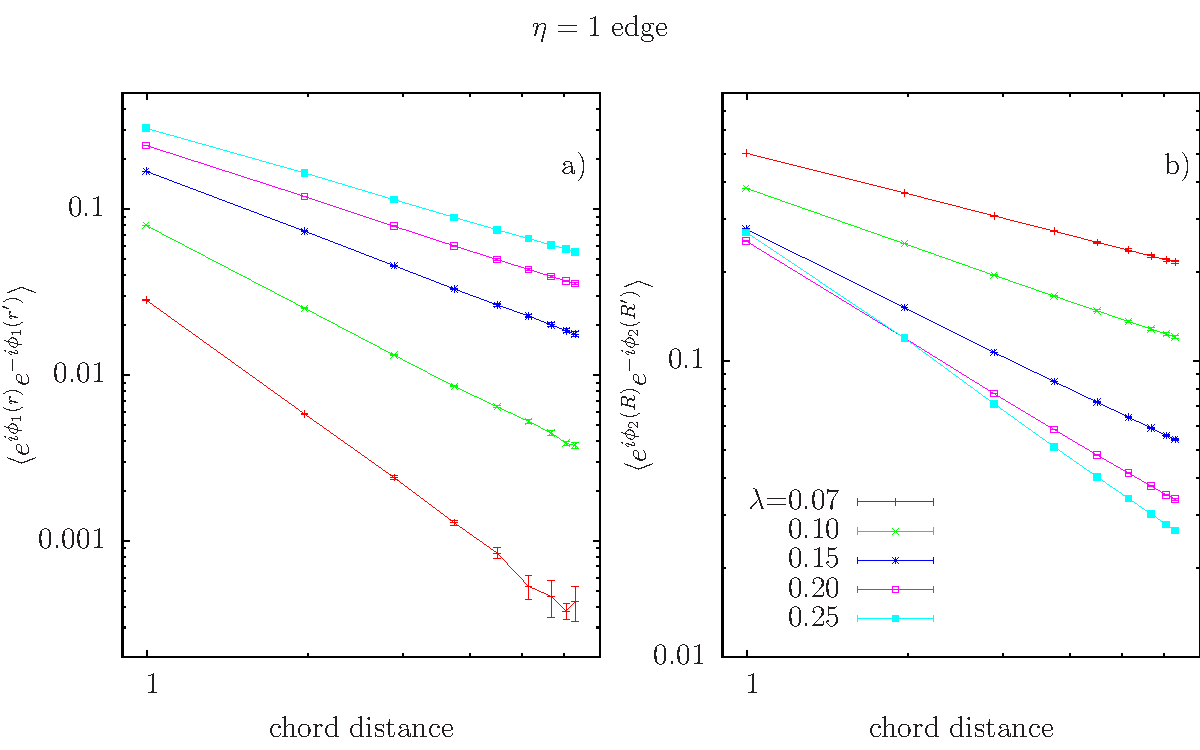
\includegraphics[width=\linewidth]{figures/onecord.eps}
\caption{ Correlation functions a) $\chi_1$ and b) $\chi_2$, plotted against the chord distance of Eq.~(\ref{cordlength}), on a log-log scale, for $\eta=1$ edge.  Error bars come from comparing runs with different initial conditions.  The straight lines imply that we have algebraic decay in the correlation functions and therefore the edge is gapless.  The slope of these lines varies with $\lambda$, and the extracted exponents are shown in Fig.~\ref{exponents}.}
\label{onegood}
\end{figure}

Figure \ref{twogood} shows the same measurements for $\eta=2$. Again we see evidence of algebraic decay with exponents which depend on $\lambda$. As above, we used the reformulation in Eq.~(\ref{Sint}) for the $\chi_2$ measurements. Note that for this data it is important to measure correlators of $\exp(i2\phi_2)$, as defined in Eq.~(\ref{Crr}). As expected, we found that single-boson correlators decay exponentially in this case, and only pair-boson correlators show algebraic decay.


From the above data we can extract the exponents of the algebraic decay. We fit the above data to the function
\begin{equation}
\chi_1(r-r')=\frac{A}{\left[\frac{L}{\pi}\sin\left(\frac{\pi|r-r'|}{L}\right)\right]^{b_{\chi_1}}},
\label{fitfunction}
\end{equation}
with $A$ and $b_{\chi_1}$ parameters of the fit. We analyzed $\chi_2$ similarly.  Figure~\ref{exponents} shows plots of these exponents for $\eta=1$ and $\eta=2$. The decay exponents for both $\chi_1$ and $\chi_2$ are slightly above the spin-wave prediction at small $\lambda$ (e.g., within 10\% for $\lambda =0.07$). At large $\lambda$ the fitted exponents differ significantly from the naive spin-wave predictions, though within an order of magnitude. In Appendix \ref{app:connections} we discuss a phenomenological understanding of the edge which predicts that the product of these exponents in the integer quantum Hall case should be equal to $1$. We can see from Fig.~\ref{exponents} that the products we measured are approximately equal to one.

\begin{figure}
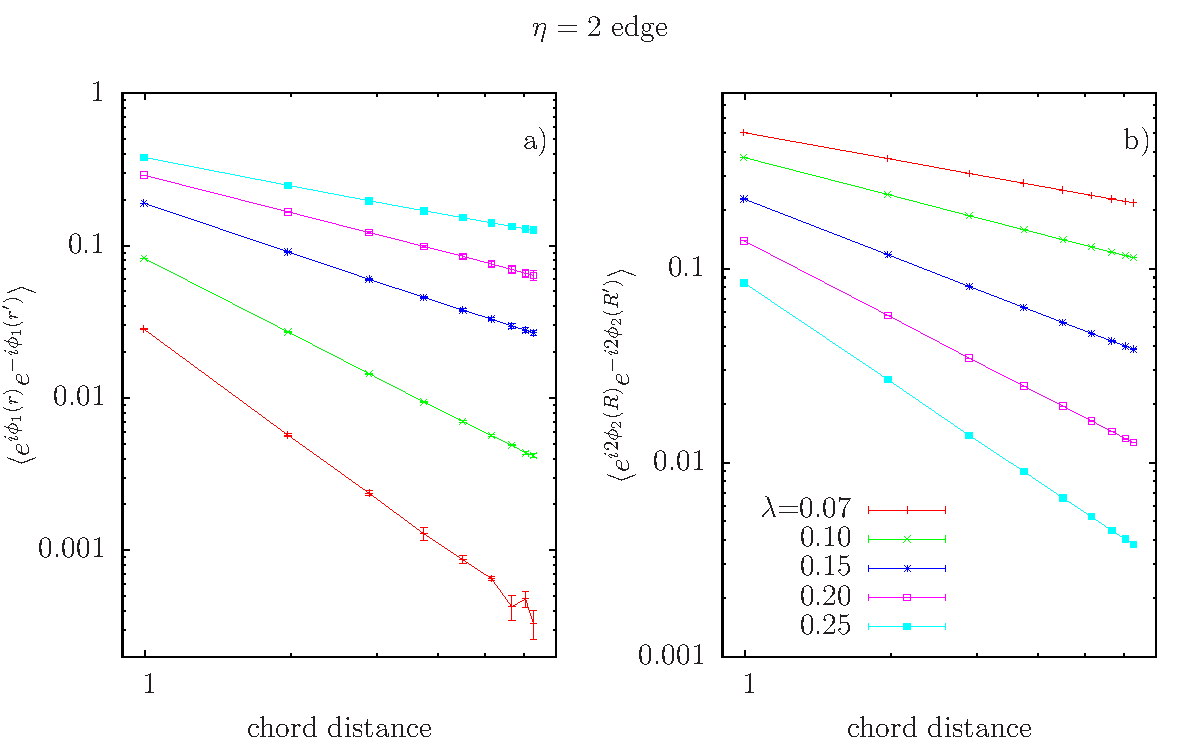
\includegraphics[width=\linewidth]{figures/twocord.eps}
\caption{ Same as Fig.~\ref{onegood}, but for $\eta=2$ edge. Once again, we see evidence for gapless modes. Note that in b) we measure pair-boson $e^{i 2\phi_2}$ correlators on the edge, while single-boson $e^{i\phi_2}$ correlators decay exponentially.
\label{twogood}}
\end{figure}

\begin{figure}
\includegraphics[width=0.6\linewidth,angle=-90]{figures/exp1.eps}
\caption{ The exponents of the algebraic decay for $\eta=1$ and $\eta=2$, extracted using the fitting function in Eq.~(\ref{fitfunction}). We see that the $b_{\chi_1}$ exponent decreases with increasing $\lambda$ while the $b_{\chi_2}$ exponent increases. The product of these exponents is also shown.
\label{exponents}}
\end{figure}

Figure~\ref{onethird} shows $\chi_2$ for $\eta=1/3$. The existence of straight lines in this plot implies that we have gapless modes in a fractional quantum Hall system. We acquired this data using the reformulation in Eq.~(\ref{Sfrac2}). We were unable to measure $\chi_1$ for the fractional cases because the decay exponents were too large. Recall that in order to have gapped $\cal{G}$ variables we need $\lambda d^2 \lesssim 0.33$; for $d^2=9$ this leads to a small $\lambda$, and the spin-wave theory estimate Eq.~(\ref{bchi1_sw}) tells us that this leads to large exponents for $\chi_1$.  The presence of the factor $d^2$ in the product $b_{\chi_1} b_{\chi_2} \approx d^2$, which we obtained here by the direct analysis, is an indirect manifestation of the fractionalization when parameter $d>1$.  Indeed, in Appendix~\ref{app:connections} we use phenomenological model of the edge and the fractionalization of the particles to show that the product of these exponents should be equal to $d^2$, while if there is no fractionalization the product will be equal to $1$. In our lattice model of the edge and the specific parameterizations of the potentials, we have found that the values of $b_{\chi_2}$ are numerically similar to those in the integer case, but the $b_{\chi_1}$ values are much larger. This implies that the product of the exponents is greater than $1$, providing indirect evidence for fractionalization.

\begin{figure}
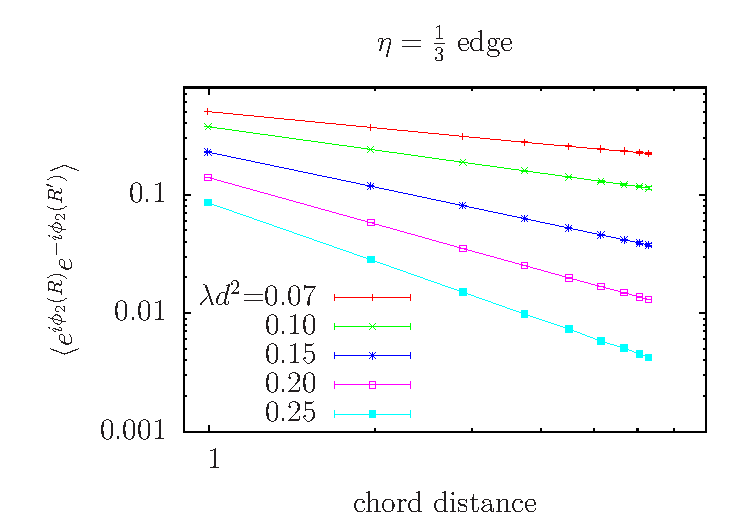
\includegraphics[width=\linewidth]{figures/thirdcord.eps}
\caption{ $\chi_2$ correlation function for $\eta=1/3$ edge, where $c=1$, $d=3$. The straight lines indicate algebraic decay for this fractional case. We were unable to obtain data for $\chi_1$ because it decayed too quickly.
\label{onethird}}
\end{figure}


%%%%%%%%%%%%%%%%%%%%%%%%%%%%%%%%%%%%%%%%%%%%%%%%%%%%%%%%%%%%%%%%%%%%%%%%%
\section{Phase diagrams}
\label{sec:reverse}

In previous works\cite{Loopy,short_range3,Gen2Loops} we have studied actions similar to that in Eq.~(\ref{kaction_2}). However, in those works we considered only the case where $\theta(k)$ was equal to a rational constant multiplied by $2\pi$. These are precisely the actions of the $\GG$ variables which appeared in Eq.~(\ref{gaction}), and from now on we will refer to them as ``statistical'' actions. The statistical variables are quasiparticles in the quantum Hall phases.  In Refs.~\cite{Loopy, short_range3} we did not attempt to connect the statistical actions to a physical system, and instead focused on their phase diagrams.  Therefore we did not specify the ``vacuum'' of physical variables as it does not affect the dynamics of the phase transitions, but it is this vacuum which carries the quantized $\sigma^{12}_{xy}$ as can be seen from Eq.~(\ref{gaction}).  Furthermore, we can now also specify physical charges of the quasiparticles.  

If we start with a statistical action with rational $\theta_{\cG}$, we can invert the change of variables procedure in Sec.~(\ref{sec::demon}) with the correct choice of $a,b,c,d$ to get an action with $\theta(k)\sim k^2$, as in Eq.~(\ref{action}), which we will from now on call the ``physical'' action. This is how we obtained the specific potentials in Eqs.~(\ref{vintro}) and (\ref{tintro}). We know from the previous works the phase diagrams of the statistical actions in terms of the variables $\GG$. We can use the change of variables in this work to describe these phase diagrams in terms of the physical variables $\JJ$. 

Recall that the specific potentials can be classified by the coefficients $c$ and $d$. When changing from the physical variables $\JJ$ to the statistical variables $\GG$, we need these coefficients as well as $a$ and $b$, but these coefficients are not independent since they must satisfy $ad-bc=1$. In particular, if we have one solution $a_0$, $b_0$ then this constraint tells us that 
\begin{eqnarray}
&&a=a_0 + mc,\nonumber\\
&&b=b_0 + md,
\label{bshift} 
\end{eqnarray} 
are also solutions if $m$ is an integer.  The statistical actions can be classified by their statistical angle, which for our specific potential choices is given by $\theta_\cG=2\pi b/d$. Therefore each physical action can be related to multiple statistical actions by our change of variables. However, these statistical actions differ only in that $\theta_\cG$ can be different by an integer multiple of $2\pi$. Such a shift will have no effect on the partition sum in the $\GG$ variables. Therefore all of the statistical actions which can be related to a given physical action have the same behavior. 

We can also see that multiple physical actions whose ratio $c/d$ differ by an integer can also be mapped to the same statistical action: that is, the actions in terms of $\cal{G}$ particles are essentially the same except for the ``background'' quantum Hall conductivity $\sigma^{12}_{xy}$ changing by an even integer. These physical actions are related to each other by adding an ``integer quantum Hall layer'' to the system without changing the properties of the fractionalized excitations. 

To begin the discussion of the broader phase diagrams of our models, it is useful to consider also the action in terms of the dual variables $\QQ_1$, $\QQ_2$:
\begin{eqnarray}
S &=& \frac{1}{2}\sum_k \frac{(2\pi)^2 }{|\vec{f}_k|^2} \left[\lambda_1|\QQ_1(k)|^2+\lambda_2|\QQ_2(k)|^2\right]\nonumber\\
&+& i\sum_k \frac{2\pi c}{d} \QQ_1(-k)\cdot \vec{a}_{\QQ2}(k),
\label{qaction}
\end{eqnarray}
where $\QQ_2=\curl\vec{a}_{\QQ2}$. This action comes from dualizing the $\cJ_1$, $\cJ_2$ variables with the specific potentials in Eqs.~(\ref{vintro}) and (\ref{tintro}). [Eq.~(15) in Ref.~\cite{short_range3} contains this action with general potentials.] This action can also be obtained by applying the modular transformation $(0, -1, 1, 0)$ to the original action. Note that the $d$ in Eq.~(\ref{qaction}) corresponds to the parameter in Eqs.~(\ref{vintro})-(\ref{tintro}), and is not related to the modular transformation used to obtain this phase.  The $\cQ$ variables are vortices with the usual long-range intra-species interactions, $v_{\cQ}(k) \sim 1/k^2$ in momentum space, and we see that these vortices are gapped for large $\lambda_1$ and $\lambda_2$.  The statistical angle in the third term of Eq.~(\ref{qaction}) is a rational number.  However, this rational number is unique to the specific choices we made in Eqs.~(\ref{vintro})-(\ref{tintro}), and small short-range modifications of the model can lead to a different statistical angle for the $\QQ$ variables.  This is unlike the rational $\theta_{\GG}$ in the quantum Hall insulators which is robust to short-range modifications of the potentials.  The difference comes from the qualitative difference when applying Eq.~(\ref{VJ}) to generic short-ranged $v(k) \sim {\rm const}$ and $\theta(k) \sim k^2$ in the cases $d=0$ (duality to only vortices) and $d\neq 0$ (more general modular transformation).

\subsection{Models with $c/d=n$, $\sigma^{12}_{xy}=2n$}
We now turn to detailed descriptions of the phase diagrams.
First we discuss the case where the conductivity in the quantum Hall phase is quantized as an even integer. In this case we start with a physical action with the potentials Eqs.~(\ref{vintro})-(\ref{tintro}) with parameters $c=n$, $d=1$ for $n$ an integer. We can get a statistical action by applying the modular transformation $(1, 0, n, 1)$, and this gives a statistical action with $\theta_{\GG}=0$ and a background Hall conductivity of $\sigma^{12}_{xy}=2n$. Therefore in the statistical action we have a system of  two uncoupled loops, which is a system that is well understood.\cite{Cha1991,Sorensen} 
In this system when $\lambda_i\lesssim 0.3325$, the variables $\GG_i$ are gapped, and when $\lambda_i$ is greater than this value the $\GG_i$ are condensed. All phase transitions are second-order XY transitions. Figure \ref{intphase} shows this phase diagram. 
Since we know the behavior of the $\GG$ variables everywhere in the phase diagram, we can now deduce the behavior of the physical $\JJ$ variables. In the lower left corner phase we have seen that the $\JJ$ variables are in a quantum Hall phase. 

To understand the rest of the phase diagram we must make more precise our earlier definitions of what makes a variable ``gapped'' or ``condensed''. When a variable is in a phase in which it is gapped, the energy cost for having large loops of that variable becomes arbitrarily large and only small loops are present. When a variable is condensed the energy cost for forming loops is small. A variable is condensed if and only if the variable dual to it is gapped. In some phases a variable will be neither condensed nor gapped in the above sense; instead the variable can be part of a composite object which is condensed or gapped. This is the situation for the $\cJ$ variables in the quantum Hall phases. We bring this out to indicate that there are more cases than just given by binary choice of $\cJ_i$ variable being gapped or condensed.  In all cases, the precise meaning is provided by finding appropriate transformation that leads to a description in terms of gapped particles only.

With this in mind, we can interpret the rest of the phase diagram. We begin with the phase in the upper-right corner, where $\lambda_1$ and $\lambda_2$ are large. We can see that in this phase the potentials seen by the $\QQ$ variables in Eq.~(\ref{qaction}) become arbitrarily large, so both of these species of variable are gapped. Therefore both species of $\JJ$ variable are condensed and this phase is a superfluid. The conductivities $\sigma^{11}_{xx}$ and $\sigma^{22}_{xx}$ diverge in this phase, while the Hall conductivity $\sigma^{12}_{xy}$ is non-universal. 

We now study the off-diagonal phases in Fig.~\ref{intphase}. For simplicity we discuss the phase in the lower right corner where $\lambda_1$ is large but $\lambda_2$ is small (in fact $\lambda_1$ can become arbitrarily large in this phase). The upper left corner is similar with the indices interchanged. From Eq.~(\ref{vintro}) we can see that when $\lambda_1\rightarrow\infty$,  $v_2(k)\rightarrow\frac{1}{\lambda_2}$. Since $\lambda_2$ is small in this phase, $v_2(k)$ can become arbitrarily large and the $\JJ_2$ variables must be gapped. In addition, we can see from Eq.~(\ref{JQreal}) that the $\QQ_1$ variables see an arbitrarily large potential and are therefore gapped, so the $\JJ_1$ variables are condensed. From the above results, we can conclude that this phase is a trivial insulator in the $\JJ_2$ variables and a superfluid in the $\JJ_1$ variables.

\begin{figure}
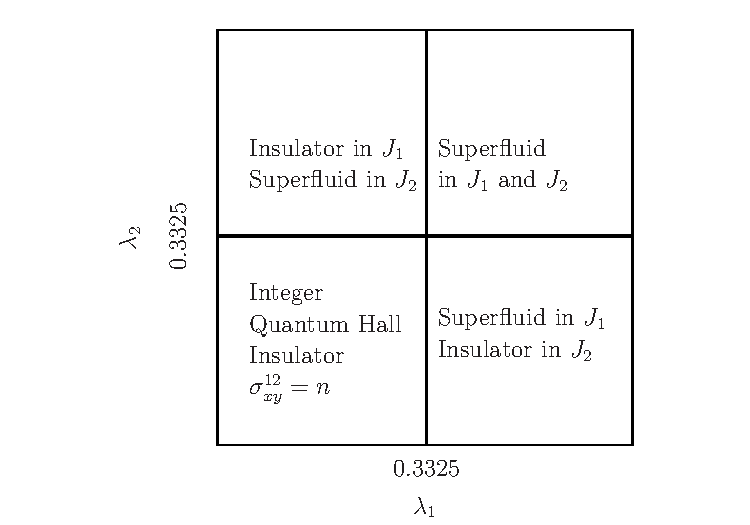
\includegraphics[width=\linewidth]{figures/intphase.eps}
\caption{The phase diagram for the model with the potentials of Eqs.~(\ref{vintro})-(\ref{tintro}) and $c=n$, $d=1$. In the lower left phase the $\GG$ variables are gapped and we have the integer quantum Hall phase with $\sigma^{12}_{xy}=2n$. In the upper right phase the $\JJ$ variables are condensed, and we have a superfluid.  In the off-diagonal phases, one of the $\cJ$ variables is condensed and the other is gapped.}
\label{intphase}
\end{figure}

Finally, we note that the specific model, Eqs.~(\ref{vintro})-(\ref{tintro}), with $c=n, d=1$ does not realize the trivial insulator phase with both $\cJ_1$ and $\cJ_2$ gapped.  Of course, we can obtain such a phase by different modifications of the potentials, e.g., by adding large repulsive pieces to both $v_1$ and $v_2$, and it would be interesting to study such models in the future.


%%%%%%%%%%%%%%%%%%%%%%%%%%%%%%%%%%%%%%%%%%%%%%%%%%%%%%%%%%%%%%%%%%%%%%%%
\subsection{Models with $d\neq 1$}
In Ref.~\cite{short_range3} we studied a statistical action with $\theta_{\cal{G}} = 2\pi/3$. The phase diagram for this model is shown in Fig.~\ref{fracphase}. In the lower left corner the $\GG$ variables are gapped and this is the fractional quantum Hall phase. Any physical action with $d=3$ and $c=1+3m$ (for $m$ an integer) can be related to this statistical action by our modular transformation; here we will discuss the case where $c=1$. In this case the change of variables needed to get from the $\JJ$ variables to the $\GG$ variables is $(0, -1, 1, 3)$. The fractional quantum Hall phase will have $\sigma^{12}_{xy}=2\cdot\frac{1}{3}$ and excitations carrying respective fractional charges of $1/3$ and mutual statistics of $2\pi/3$.

We know from our previous numerical study\cite{short_range3} that in the middle phase the variables dual to the $\GG$ variables are gapped. 
We can also compute the action for the variables dual to the $\GG$ variables and see that it has the same potential as the action for the $\JJ$ variables. The two actions also have values of $\theta(k)$ which differ only by an integer multiple of $2\pi$. Such difference will translate to factors $e^{2\pi i}$ in the partition sum and therefore will not contribute. Therefore if the variables dual to the $\GG$ variables are gapped then the $\JJ$ variables should also be gapped. Therefore this middle phase is a trivial insulator in the $\JJ$ variables. This can be confirmed by measuring the conductivity numerically in this phase. 

In the upper right corner phase we can see from Eq.~(\ref{qaction}) that the $\cQ$ variables are gapped,  and therefore the $\JJ$ variables are condensed and this phase is a superfluid.  In our previous work\cite{short_range3} we found that transition between the trivial insulator and the superfluid is a pair of XY transitions, while we found more complicated behavior at the fractional quantum Hall-trivial insulator transition. 

The structure described in the previous paragraph holds for any set of physical variables which can be mapped to a statistical action with $\theta_\cG=2\pi/m$, with $m$ an integer. %\cite{footnoten2}.
One exception is $m=2$, where our specific model with $c=1, d=2$ has an additional symmetry in the $\cG$ variables which prevents the existence of the middle phase, cf.~Fig.~1 in Ref.~\cite{Loopy}.  This is discussed in detail in Refs.~\cite{Loopy, Gen2Loops}, while here we note that generic perturbations to our original model will break this symmetry and open a sliver of the trivial phase in the phase diagram.

Finally, for more complicated fractions $c/d$, our model will have multiple phases in the middle of the phase diagram, resembling hierarchy of phases that we found in $U(1) \times U(1)$ loop models with marginally long-ranged interactions and modular invariance.\cite{Gen2Loops}  We expect that the ``middle'' phase at the largest $\lambda$ is a trivial insulator, while the other phases are various quantum Hall states.  For example, in our model Eqs.~(\ref{vintro})-(\ref{tintro}) with $c=2, d=5$, we found the following sequence of phases upon increasing $\lambda_1 = \lambda_2$: fractional quantum Hall insulators $\sigma^{12}_{xy} = 2\cdot 2/5$ and $\sigma^{12}_{xy} = 2\cdot 1/2$, trivial insulator $\sigma^{12}_{xy} = 0$, and superfluid.  It would be interesting to explore such phase diagrams and phase transitions in more detail in the future.

\begin{figure}
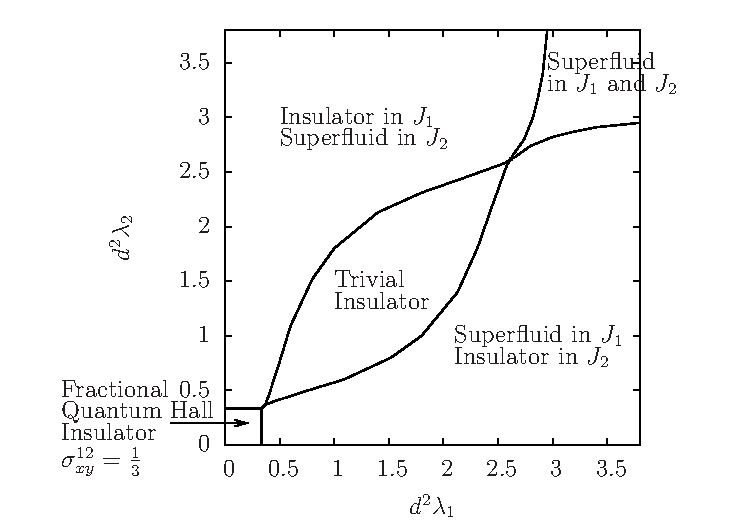
\includegraphics[width=\linewidth]{figures/fracphase.eps}
\caption{The phase diagram for the model with $c=1,d=3$. In the lower left phase the $\GG$ variables are gapped and we have a fractional quantum Hall phase with $\sigma^{12}_{xy}=2\cdot\frac{1}{3}$. In the upper right phase the $\JJ$ variables are condensed, which implies a superfluid. In the middle phase the $\JJ$ variables are gapped and we have a trivial insulator. This figure is reproduced from Ref.~\cite{short_range3}, but the phases have been re-interpreted in terms of the physical variables discussed in this work.}
\label{fracphase}
\end{figure}


%%%%%%%%%%%%%%%%%%%%%%%%%%%%%%%%%%%%%%%%%%%%%%%%%%%%%%%%%%%%%%%%%%
\section{Hamiltonian formulation}
\label{app:H}
Throughout the main text, we worked with the Euclidean action formulation of the model.  The action for the physical currents is local in (2+1)D space-time and is very convenient for analysis.  However, it is natural to ask whether this action can be realized as a path integral of a local Hamiltonian in 2d.\cite{Matthew_Alexei_thanks}  Below we provide an example of such a Hamiltonian.

We first specify the physical Hilbert space.  Our degrees of freedom reside on two inter-penetrating square lattices as shown in Fig.~\ref{fig:H}.  We place quantum U(1) rotors on sites $\br$ of the first square lattice.  The rotors are described by $2\pi$-periodic phase variables $\hat{\phi}_1(\br)$ and conjugate integer number variables $\hat{n}_1(\br)$, with commutation relations $[\hat{\phi}_1(\br), \hat{n}_1(\br')] = i \delta_{\br\br'}$.  We place another set of U(1) rotors, described by $\hat{\phi}_2(\bR)$ and $\hat{n}_2(\bR)$, on sites $\bR$ of the second (dual) square lattice.  Finally, we place harmonic oscillators, described by $\hat{\chi}_\ell$ and $\hat{\pi}_\ell$, on centers of links of the first square lattice, which are also centers of links of the second square lattice, e.g., $\ell = <\br, \br + \hat{\bx}> = <\bR, \bR + \hat{\by}>$ as illustrated in Fig.~\ref{fig:H}.  Here $\hat{\chi}_\ell$ are real-valued coordinate variables and $\hat{\pi}_\ell$ are conjugate momentum variables, $[\hat{\chi}_\ell, \hat{\pi}_{\ell'}] = i\delta_{\ell\ell'}$.  Looking ahead, we will use a path integral containing both $\chi_\ell$ and $\pi_\ell$.  We will view the coordinate variables as fields on the links of the first lattice,
\begin{equation}
\hat{\alpha}_{1j}(\br) \equiv \hat{\chi}_{\br, \br + \hat{\bj}} ~,
\end{equation}
$\hat{\bj} = \hat{\bx}$ or $\hat{\by}$, while we will view the conjugate momentum variables as fields on the links of the second lattice,
\begin{equation}
\hat{\alpha}_{2j}(\bR) = \epsilon_{jk} \hat{\pi}_{\br, \br + \hat{\bk}} ~.
\end{equation}
Here $\epsilon_{xy} = -\epsilon_{yx} = 1$ is the 2d antisymmetric tensor and $<\bR, \bR + \hat{\bj}>$ and $<\br, \br + \hat{\bk}>$ are crossing links.\cite{footnoteKitaev}
Note that in this Appendix we adopt the following notation:  Spatial lattice sites are labeled with bold face, e.g., $\br, \bR$.  Spatial directions are labeled with Roman letters, e.g., $j, k$; space-time directions that appear later will be labeled with Greek letters, e.g., $\mu, \nu$.  Oriented fields residing on spatial links are viewed as spatial vectors and are labeled with bold face, e.g., ${\bm \alpha_1}, {\bm \alpha_2}$.

%\begin{figure}[t!]
%\input{H.pstex_t}
%\caption{Our Hamiltonian Eq.~(\ref{H}) has U(1) rotors residing on sites $\br$ of the direct square lattice and U(1) rotors residing on sites $\bR$ of the dual lattice.  We also have harmonic oscillators residing on crosses $\ell$ of the links of the two lattices.  The first and second U(1) systems are coupled to the oscillator position and momentum variables respectively as if the latter were gauge fields.\cite{footnoteKitaev}  With appropriate choices of parameters and additional charge-flux couplings, we can induce condensations of bound states of charges and vortices leading to the quantum Hall states discussed in the main text.}
%\label{fig:H}
%\end{figure}


Our Hamiltonian is:
\begin{eqnarray}
\label{H}
\hat{H} &=& \hat{H}_{h1} + \hat{H}_{h2} + \hat{H}_{u1} + \hat{H}_{u2} + \hat{H}_\chi + \hat{H}_\pi ~,\\
\hat{H}_{h1} &=& -\sum_{\br, j} h_1 \cos[\nabla_j \hat{\phi}_1(\br) - e_1 \hat{\alpha}_{1j}(\br)] ~,\\
\hat{H}_{h2} &=& -\sum_{\bR, j} h_2 \cos[\nabla_j \hat{\phi}_2(\bR) - e_2 \hat{\alpha}_{2j}(\bR)] ~,\\
\hat{H}_{u1} &=& \frac{1}{2} \sum_\br u_1 \left[\hat{n}_1(\br) + g_1 ({\bm \nabla} \wedge \hat{\bm \alpha}_2)(\br) \right]^2 ~,\\
\hat{H}_{u2} &=& \frac{1}{2} \sum_\bR u_2 \left[\hat{n}_2(\bR) + g_2 ({\bm \nabla} \wedge \hat{\bm \alpha}_1)(\bR) \right]^2 ~,\\
\hat{H}_\chi &=& \sum_\ell \frac{\kappa\, \hat{\chi}_\ell^2}{2} ~, \quad
\hat{H}_\pi = \sum_\ell \frac{\hat{\pi}_\ell^2}{2m} ~.
\end{eqnarray}
Here we introduced various parameters such as boson hopping amplitudes $h_1$ and $h_2$, on-site energies $u_1$ and $u_2$, and oscillator parameters $\kappa$ and $m$.  The hopping terms couple the boson phases and the oscillators as if the latter were ``gauge fields.''  The on-site terms couple the boson numbers and appropriate fluxes of the ``gauge fields'': e.g., flux ${\bm \nabla} \wedge \hat{\bm \alpha}_1 \equiv \nabla_x \hat{\alpha}_{1y} - \nabla_y \hat{\alpha}_{1x}$ is associated with a plaquette of the first lattice, or, equivalently a site $\bR$ of the dual lattice, and is coupled with the boson number $\hat{n}_2(\bR)$ on that site.  The corresponding parameters $e_1, e_2, g_1, g_2$ will be chosen later. 
Here we emphasize that the model is local in the physical variables (i.e., it is not a gauge theory), in the same spirit as Kitaev's toric code model.

We develop imaginary-time path integral by using Trotter decomposition and insertions of unity as follows:
\begin{eqnarray*}
e^{-\delta\tau \hat{H}} &\approx& e^{-\delta\tau (\hat{H}_{u1} + \hat{H}_{h2} + \hat{H}_\pi)} e^{-\delta\tau (\hat{H}_{h1} + \hat{H}_{u2} + \hat{H}_\chi)}
= ~\mathbbm{1}_{\tau + \delta\tau}~ e^{-\delta\tau (\hat{H}_{u1} + \hat{H}_{h2} + \hat{H}_\pi)} ~\mathbbm{1}_{\tau + \frac{\delta\tau}{2}}~ e^{-\delta\tau (\hat{H}_{h1} + \hat{H}_{u2} + \hat{H}_\chi)} ~\mathbbm{1}_{\tau} ~,\\
\mathbbm{1}_{\tau} &=&
\int_{-\pi}^\pi D\phi_1(\br, \tau)
\sum_{n_2(\bR, \tau) = -\infty}^\infty
\int_{-\infty}^\infty D\chi_\ell(\tau) ~
\Big|   \phi_1(\br, \tau), n_2(\bR, \tau), \chi_\ell(\tau) \Big\ra
\Big\la \phi_1(\br, \tau), n_2(\bR, \tau), \chi_\ell(\tau) \Big| ~,\\
\mathbbm{1}_{\tau_\half \equiv \tau + \frac{\delta\tau}{2}} &=&
\sum_{n_1(\br, \tau_\half) = -\infty}^\infty
\int_{-\pi}^\pi D\phi_2(\bR, \tau_\half) 
\int_{-\infty}^\infty D\pi_\ell(\tau_\half) ~
\Big|   n_1(\br, \tau_\half), \phi_2(\bR, \tau_\half), \pi_\ell(\tau_\half) \Big\ra
\Big\la n_1(\br, \tau_\half), \phi_2(\bR, \tau_\half), \pi_\ell(\tau_\half) \Big| ~.
\end{eqnarray*}
Here we used one set of variables on ``integer'' time slices $\tau = {\rm int} \times \delta\tau$ and conjugate variables on ``half-integer'' time slices $\tau_\half \equiv \tau + \delta\tau/2$.  We also arranged the Trotter decomposition so that the pieces of the Hamiltonian act as $c$-numbers on the kets of the above insertions of unity.  Throughout, we omit normalization constants.  The remaining inputs to complete the path integral formulation in the above variables are overlaps such as
\begin{eqnarray}
\big\la \chi_\ell(\tau + \delta\tau) \big| \pi_\ell(\tau_\half) \big\ra
\big\la \pi_\ell(\tau_\half) \big| \chi_\ell(\tau) \big\ra &=& e^{i \pi_\ell(\tau_\half) [\chi_\ell(\tau + \delta\tau) - \chi_\ell(\tau)]}
= e^{i \alpha_{2k} \epsilon_{kj} \nabla_\tau \alpha_{1j}} ~,
\quad {\rm for~} \ell = <\br, \br+\hat{\bj}>, ~ \\
\big\la \phi_1(\br, \tau + \delta\tau) \big| n_1(\br, \tau_\half) \big\ra
\big\la n_1(\br, \tau_\half) \big| \phi_1(\br, \tau) \big\ra &=&
e^{i n_1(\br, \tau_\half) [\phi_1(\br, \tau + \delta\tau) - \phi_1(\br, \tau)]}
= e^{i \cJ_{1\tau} \nabla_\tau \phi_1} ~,
\end{eqnarray}
ans similarly for the second rotor variables.

In the action, we have phase variables $\phi_1(\br, \tau)$ residing on sites $(\br, \tau)$ of a (2+1)D cubic lattice and $\phi_2(\bR, \tau_\half)$ residing on sites $(\bR, \tau_\half)$ of a dual cubic lattice (in the main text, such space-time points are labeled simply $r$ and $R$).  We also have boson number variables $n_1(\br, \tau_\half)$ and $n_2(\bR, \tau)$, which we can view as residing on temporal links of the first and second (dual) cubic lattices respectively and write as temporal components of boson three-currents, $\cJ_{1\tau}(\br, \tau) \equiv n_1(\br, \tau_\half)$ and $\cJ_{2\tau}(\bR, \tau_\half) \equiv n_2(\bR, \tau + \delta\tau)$.  We introduce spatial current components using an approach familiar in treatments of XY models; namely, we interpret the cosine terms in $\hat{H}_{h1}$ and $\hat{H}_{h2}$ as so-called Villain cosines and write, e.g.,
\begin{eqnarray*}
&& e^{\delta\tau h_1 \cos[\nabla_j \phi_1(\br, \tau) - e_1 \alpha_{1j}(\br, \tau)]} \\
&& \to \sum_{\cJ_{1j}(\br, \tau) = -\infty}^\infty e^{-\frac{\cJ_{1j}^2}{2 \delta\tau h_1} + i \cJ_{1j} [\nabla_j \phi_1 - e_1 \alpha_{1j}]} ~.
\end{eqnarray*}
We can now integrate over the phase degrees of freedom and obtain current conservation conditions, $\vec{\nabla} \cdot \vcJ_1 \equiv \sum_{\mu=x, y, \tau} \nabla_\mu \cJ_{1\mu} = 0$, and similarly for the three-current $\vcJ_2$.
Here and below, arrows over symbols denote three-vectors such as $\vcJ_1 = (\cJ_{1x}, \cJ_{1y}, \cJ_{1\tau})$, while bold symbols refer to spatial parts such as ${\bm \cJ}_1 = (\cJ_{1x}, \cJ_{1y})$.

We still have the oscillator variables, now labeled ${\bm \alpha}_1(\br, \tau)$ and ${\bm \alpha}_2(\bR, \tau_\half)$ and residing on spatial links of the first and second cubic lattices.  At this point, we could also integrate over these variables and obtain an action in terms of the boson three-currents only.  To facilitate the integration and show the connection with the loop models in the main text, we will first write the on-site terms by introducing auxiliary fields labeled $\alpha_{1\tau}$ and $\alpha_{2\tau}$ residing on the temporal links of the first and second cubic lattices respectively, e.g.:
\begin{eqnarray*}
&& e^{-\frac{\delta\tau u_2}{2} \left[\cJ_{2\tau}(\bR, \tau_\half) + g_2 ({\bm \nabla} \wedge {\bm \alpha}_1)(\bR, \tau_\half) \right]^2} \\
&& = \int_{-\infty}^\infty d\alpha_{2\tau}(\bR, \tau_\half) e^{-\frac{\alpha_{2\tau}^2}{2 \delta\tau u_2} - i \alpha_{2\tau} \left[J_{2\tau} + g_2 ({\bm \nabla} \wedge {\bm \alpha}_1) \right]} ~.
\end{eqnarray*}
For brevity, we often omit the lattice coordinates on the fields and imply precise geometric relation between objects on different lattices: e.g., an oriented plaquette on one lattice is also associated with a unique oriented bond on the other lattice crossing this plaquette.

Putting everything together, the final action takes the form
\begin{eqnarray*}
&& S[\valpha_1, \valpha_2, \vcJ_1, \vcJ_2] = 
\sum \left[ \frac{\delta\tau \kappa\, {\bm \alpha}_1^2}{2} + \frac{\alpha_{1\tau}^2}{2\delta\tau u_1} + \frac{\delta\tau {\bm \alpha}_2^2}{2m} + \frac{\alpha_{2\tau}^2}{2\delta\tau u_2} \right]
+ \sum \left[\frac{{\bm \cJ}_1^2}{2\delta\tau h_1} + \frac{{\bm \cJ}_2^2}{2\delta\tau h_2} \right] \\
&&\quad + i \sum \left[ (\nabla_\tau{\bm \alpha}_1) \wedge {\bm \alpha}_2 + g_1 \alpha_{1\tau} ({\bm \nabla} \wedge {\bm \alpha}_2) + g_2 \alpha_{2\tau} ({\bm \nabla} \wedge {\bm \alpha}_1) \right]
+ i \sum \left[ e_1 {\bm \cJ}_1 \cdot {\bm \alpha}_1 + \cJ_{1\tau} \alpha_{1\tau} + e_2 {\bm \cJ}_2 \cdot {\bm \alpha}_2 + \cJ_{2\tau} \alpha_{2\tau} \right] ~. 
\end{eqnarray*}
Here the wedge operator is ${\bm v}_1 \wedge {\bm v}_2 \equiv \sum_{j,k} \epsilon_{jk} v_{1j} v_{2k} = v_{1x} v_{2y} - v_{1y} v_{2x}$.
By rescaling ${\bm \alpha}_1 = {\bm \alpha}^\prime_1/e_1$ and similarly for  ${\bm \alpha}_2$, and choosing, e.g., $e_1 = e_2 = 1/g_1 = 1/g_2 = \sqrt{2\pi d/c}$, we obtain essentially the same action as in Eq.~(\ref{preal}) in the main text.  The only difference from the main text is that there are additional local current interactions containing $h_1$ and $h_2$ couplings, and to make the actions identical we only need to take $h_1$ and $h_2$ large.  In particular, the model is in the ``$c/d$'' Quantum Hall phase for sufficiently small $\kappa$ and sufficiently large $m$ and large $u_1, u_2$.
Thus, we have provided a Hamiltonian realization for our Quantum Hall phases.

We can also carry out this derivation when the parameters $h_{1,2}, u_{1,2}, \kappa, m, e_{1,2}, g_{1,2}$ vary in space; in particular, we can study a boundary between Quantum Hall and trivial insulators.
Note that there is significant freedom in how to vary the parameters to achieve different phases even within the specific model.  For example, we can obtain a trivial insulator by taking $e_{1,2}$ and $g_{1,2}$ to be zero while also taking the hopping amplitudes $h_{1,2}$ to be small and on-site potentials $u_{1,2}$ large.
Alternatively, we can take $e_{1,2}$ to be very large while $g_{1,2} \to 0$ and can reach the trivial insulator this way even when the bare hopping amplitudes $h_{1,2}$ are large (in this case, the boson propagation is scrambled by strong phase coupling to the oscillators).  The latter route is closer to the model we used in the main text when discussing a boundary between Quantum Hall and trivial insulators.  Such a boundary model in the present Hamiltonian approach will in general differ from that in the main text.  Indeed, in the Chern-Simons-like piece for the rescaled $\valpha^\prime_{1,2}$ variables,
\begin{equation*}
i \sum [ \frac{(\nabla_\tau {\bm \alpha}^\prime_1) \wedge {\bm \alpha}^\prime_2}{e_1 e_2} + g_1 \alpha_{1\tau} ({\bm \nabla} \wedge \frac{{\bm \alpha}^\prime_2}{e_2}) + g_2 \alpha_{2\tau} ({\bm \nabla} \wedge \frac{{\bm \alpha}^\prime_1}{e_1}) ] ~,
\end{equation*}
the spatially varying $e$ and $g$ couplings can appear non-trivially under spatial derivatives, and the action in general cannot be cast in the form of Eq.~(\ref{JQreal}).  However, we can find a pattern of couplings that will reproduce our boundary model in the main text:  If we take $1/e_a = g_a = \sqrt{c/(2\pi d)}$ for $x\in [x_{aL}, x_{aR}]$ and $1/e_a = g_a = 0$ otherwise, and take the region $[x_{2L}, x_{2R}]$ to be inside the region $[x_{1L}, x_{1R}]$, we eliminate terms with non-desired derivatives of the couplings and can recast the Chern-Simons-like piece for the rescaled $\valpha^\prime_{1,2}$ variables into the form of Eq.~(\ref{JQreal}) with $\eta(R) = c/d$ inside $[x_{2L}, x_{2R}]$ and zero outside.  Thus, we have also provided a Hamiltonian realization of the boundary model used in the main text.

While we universally expect gapless boson correlations on the boundary, detailed aspects can be different for different realizations.  In this paper, we have focused on the crude demonstration of the gaplessness for the specific boundary model in the main text.  In future work, it would be interesting to examine different realizations and systematically explore all aspects of possible edge theories.

%%%%%%%%%%%%%%%%%%%%%%%%%%%%%%%%%%%%%%%%%%%%%%%%%%%%%%%%%%%%%%%%%%%%%%%%
\section{Discussion}
In this work we have presented physical $U(1) \times U(1)$ bosonic models which realize insulating phases with a quantized Hall conductivity that can take both integer and fractional values. 
In the fractional case, we also have excitations carrying fractionalized charges and non-trivial mutual statistics. We have shown how to study these models in Monte Carlo and found evidence for gapless edge modes. We have also presented broader phase diagrams of our models.

The action in Eq.~(\ref{action}) can be derived from a local Hamiltonian, as shown in Appendix \ref{app:H}. When we included an edge in our action by varying $\eta(R)$ in Eq.~(\ref{JQreal}), we do not know precisely how that edge is realized in the physical Hamiltonian. It is possible that this method of including an edge changes the Hamiltonian near the edge in such a way as to create gapless modes which are not due to the bulk topological state of the system on one side.  For example, a local strengthening of boson hopping along the edge could lead to gapless (1+1)D Luttinger liquid modes.  Irrespective of the microscopic details, the edges that we studied do produce the quantum Hall $\sigma^{12}_{xy}$, so at least some of the observed properties are due to the topology of the bulk phases.  Including edges using different methods, and confirming that the observed gapless properties are not artifacts of the method used in this work, is a possible subject of future research. There is however some evidence that our gapless modes are due to topological effects. In the $\eta=1/3$ case we expect topological gapless modes to exist on the edge in the bottom left corner of the phase diagram, but not in the middle phase. This is precisely the behavior which we have observed, with gapless modes disappearing beyond $\lambda d^2=0.35$. In addition, we have observed gaplessness in both $\phi_1$ and $\phi_2$ variables (for the integer case where both signals could be detected), which is what we expect if the gapless modes are topological, and in qualitative agreement with the phenomenological $K$-matrix theory of the edge in Appendix~\ref{app:connections}. 

Our work allows the numerical study of interacting topological insulator phases, and therefore may be able to address many questions about such phases. For example, we could investigate the effect of disorder and other perturbations on the gapless edge states. We could also study transitions between different topological phases. In Ref.~\cite{short_range3} we have observed unusual behavior at the fractional quantum Hall-trivial insulator transition, which could be studied more closely. In addition, our model can realize transitions between different fractional quantum Hall states, as well as transitions between integer quantum Hall states and trivial insulators, which are of recent interest.\cite{GroverVishwanath2012, LuLee2012_QPT}
More generally, it would be interesting to see what other interacting topological phases can allow unbiased numerical studies. Furthermore, since ideas in the present work do not rely on Chern-Simons construction specific to (2+1)D, they may be more readily extended to studies of such phases in higher dimensions.\cite{VishwanathSenthil2012, KeyserlingkBurnellSimon2013, XuSenthil2013, Wen2013}

%%%%%%%%%%%%%%%%%%%%%%%%%%%%%%%%%%%%%%%%%%%%%%%%%%%%%%%%%%%%%%%%%%%%
%%%%%%%%%%%%%%%%%%%%%%%%%%%%%%%%%%%%%%%%%%%%%%%%%%%%%%%%%%%%%%%%%%%%
%\appendix
%\section{Relation to other approaches}
%\label{app:connections}
%In the main text, we obtained the physics of our models directly using exact transformations.  Here we point out connections to effective field-theoretic approaches that may be more familiar to the readers.  Our models can provide rigorous framing and testing grounds for such approaches.


%%%%%%%%%%%%%%%%%%%%%%%%%%%%%%%%%%%%%%%%%%%%%%%%%%%%%%%%%%%%%%%%%%%%
%\subsection{Relation to non-linear sigma models with topological terms}
%Let us consider our model in terms of the dual vortex variables $\cQ_{1,2}$, which has an action given by Eq.~(\ref{qaction}).  As argued in Ref.~\cite{Senthil2006_theta}, a similar vortex loop model arises in an $O(2) \times O(2)$ theory with a topological term with $\theta = \theta_\cQ$.  We see that integer quantum Hall states in our model ($c=n, d=1$) correspond to $\theta_\cQ = 2\pi n$, as proposed in Ref.~\cite{SenthilLevin2012}.  We also see that fractional ``$c/d$'' Quantum Hall states constructed in this paper correspond to $\theta_\cQ = 2\pi c/d$.  Our models thus provide lattice regularizations of such non-linear sigma models with topological terms.  Here we want to emphasize that such models do not correspond to a single phase; instead, they can have rich phase diagrams, as illustrated in the main text.

%Using our action in terms of the $\cQ_{1,2}$ variables and Eq.~(26) from Ref.~\cite{short_range3}, we can obtain an equivalent formulation of the original physical current model as
%\begin{widetext}
%\begin{eqnarray}
%S[\valpha_{q1}, \valpha_{q2}, \vcJ_1, \vcJ_2] &=&
%\frac{1}{2} \sum_k
%\frac{\lambda_1 |[\vec{\nabla} \times \valpha_{q1}](k)|^2
%      + \lambda_2 |[\vec{\nabla} \times \valpha_{q2}](k)|^2}{ |\vec{f}_k|^2}
%+ i\sum_k \frac{c}{2\pi d} [\vec{\nabla} \times \valpha_{q1}](-k) \cdot \valpha_{q2}(k) \\
%&& + i \sum_k \left[\vcJ_1(-k) \cdot \valpha_{q1}(k)
%                    + \vcJ_2(-k)\cdot \valpha_{q2}(k)\right] ~.
%\nonumber
%\end{eqnarray}
%\end{widetext}
%The above equation is an intermediate step in the exact duality transformation between $\vcQ_{1,2}$ and $\vcJ_{1,2}$, where $\valpha_{q1,2}$ are auxiliary real-valued gauge fields encoding conserved real-valued currents that appear in the duality transformation, see Appendix in Ref.~\cite{short_range3}.  We can interpret these gauge fields as mediating the interactions of the physical currents $\vcJ_{1,2}$.  The action for the gauge fields has a mutual Chern-Simons term but also explicit ``mass terms''; the latter make the physical current interactions short-ranged, as desired.

%Since the gauge fields are real-valued (non-compact), the above representation implies that our model action is unitary, i.e., it can arise as a path integral of a quantum Hamiltonian\cite{Gukov2004, Hansson2004} (see also direct demonstration in Appendix~\ref{app:H}).  In fact, this is true for arbitrary formal parameter $c/d \to \eta$.  Note, however, that any such model can still have only rational Quantum Hall phases of the type described in the main text, with different rational $\sigma^{12}_{xy} = 2c'/d'$ in different regimes.  Indeed, the available transformations to new gapped variables are modular transformations with integer entries $(a', b', c', d')$ and can only produce gapped Quantum Hall phases with rational $\sigma^{12}_{xy}$.  We can still apply this method to analyze microscopic models with any $\eta$, where it is natural to try rational approximants $c'/d'$ to $\eta$ and hence natural to expect rich phase diagram,\cite{Cardy1982, Shapere1989, Gen2Loops} while details require case-by-case study.

%Finally, we note close relation to one of the reformulations in the main text.  Since we ultimately want the action in terms of only the conserved currents $\vcJ_1$ and $\vcJ_2$, we can perform the integration over the gauge fields $\valpha_{q1}$ and $\valpha_{q2}$ in any gauge.  For example, we can use the gauge $\vec{\nabla} \cdot \valpha = 0$ and implement it as follows:  We replace $(\vec{\nabla} \times \valpha)^2 \to (\vec{\nabla} \times \valpha)^2 + \xi (\vec{\nabla} \cdot \valpha)^2$, perform unrestricted integration over the $\valpha$ variables, and take the limit of large $\xi$.  We can check that as long as the currents $\vcJ$ are conserved everywhere, the unrestricted integration over $\valpha$ gives an action independent of $\xi$.  (A note of caution: the above statement does not hold when the currents have sources and sinks -- indeed, boson Green's functions are gauge-dependent.)  Taking specific value $\xi=1$ gives Eq.~(\ref{preal}) in the main text.
%In the partition sum, we integrate independently over real-valued fields $\valpha_{1,2}$, and we can check directly that this gives the postulated model without the recourse to the dual description.    We reiterate that the action Eq.~(\ref{preal}) is not a gauge theory; rather, $\valpha_{1,2}$ are some local ``oscillator'' fields mediating short-ranged interactions of the physical currents $\vcJ_{1,2}$.  In Appendix~\ref{app:H}, we will show how such an action can arise as a path integral of a quantum Hamiltonian with only local degrees of freedom and local interactions.


%%%%%%%%%%%%%%%%%%%%%%%%%%%%%%%%%%%%%%%%%%%%%%%%%%%%%%%%%%%%%%%%%%%%
%\subsection{Relation to $K$-matrix theories}
%\label{subsec:Kmatrix}
%Here we show that our modular transformation analysis can be viewed as a derivation of a $K$-matrix-like theory, albeit with some non-standard structure in general.  The transformation consists of 
%1) duality from $\vcJ_1$ to $\vcQ_1$;
%2) change of variables $\vcQ_1 = d \vcF_1 - b \vcG_2, \vcJ_2 = c \vcF_1 - a \vcG_2$ [inverse of Eq.~(\ref{modularshift})];
%and 3) duality from $\vcF_1$ to $\vcG_1$.
%We show all steps starting with the physical action and give detailed explanations below:
%\begin{widetext}
%\begin{eqnarray}
%&& S[\vcJ_1, \vcJ_2; \vAext_1, \vAext_2] = S_{\rm s.r.}\left[\vcJ_1, \vcJ_2\right]
%+ i \sum \left[\vcJ_1 \cdot \vAext_1 + \vcJ_2 \cdot \vAext_2 \right]; \nonumber \\
%%%
%&& S_1[\vbeta, \vcQ_1, \vcJ_2; \vAext_1, \vAext_2] = S_{\rm s.r.}\left[\frac{\vec{\nabla} \times \vbeta}{2\pi}, \vcJ_2 \right]
%+ i \sum \left[\frac{\vec{\nabla} \times \vbeta}{2\pi} \cdot \vAext_1 + \vcJ_2 \cdot \vAext_2 + \vcQ_1 \cdot \vbeta \right]; \nonumber \\
%%%
%&& S_2[\vbeta, \vcF_1, \vcG_2; \vAext_1, \vAext_2] = S_{\rm s.r.}\left[\frac{\vec{\nabla} \times \vbeta}{2\pi}, c \vcF_1 - a \vcG_2 \right]
%+ i \sum \left[\frac{\vec{\nabla} \times \vbeta}{2\pi} \cdot \vAext_1 + \vcF_1 \cdot (d \vbeta + c \vAext_2) - \vcG_2 \cdot (b \vbeta + a \vAext_2) \right]; \nonumber \\
%%%
%&& S_3[\vbeta, \vgamma, \vcG_1, \vcG_2; \vAext_1, \vAext_2] = S_{\rm s.r.}\left[\frac{\vec{\nabla} \times \vbeta}{2\pi}, c \frac{\vec{\nabla} \times \vgamma}{2\pi} - a \vcG_2 \right] + \nonumber \\
%&& \quad\quad ~+~ i \sum \left[d \frac{\vec{\nabla} \times \vgamma}{2\pi} \cdot \vbeta + \frac{\vec{\nabla} \times \vbeta}{2\pi} \cdot \vAext_1 + c \frac{\vec{\nabla} \times \vgamma}{2\pi} \cdot \vAext_2 \right]
%+ i \sum \left[\vcG_1 \cdot \vgamma - \vcG_2 \cdot (b \vbeta + a \vAext_2) \right]. \label{SKmatr}
%\end{eqnarray}
%\end{widetext}
%First, we do not need to specify the microscopic action $S_{\rm s.r.}$ with short-ranged interactions other than that it gives the desired ``$c/d$'' phase for some parameters; we carry $S_{\rm s.r.}$ throughout to better display all connections.  We also keep track of the external vector potentials $\vAext_{1,2}$.  At each step, we show explicitly degrees of freedom that form the partition sum.

%1) We treat the duality from the boson current $\vcJ_1$ to vortex current $\vcQ_1$ as a reformulation of the partition sum replacing $\vcJ_1 \to \vec{\nabla} \times \vbeta/(2\pi)$, with real-valued gauge field $\vbeta$, while keeping the information about the integer-valuedness of $\vcJ_1$ with the help of new integer-valued current $\vcQ_1$ as shown in $S_1$ (see, e.g.,~Appendix in Ref.~\cite{short_range3}).
%2) Here we change to new independent currents $\vcF_1, \vcG_2$, which is a valid transformation for $(a, b, c, d)$ forming a modular matrix.
%3) Finally, we perform formal duality from $\vcF_1$ to $\vcG_1$ as in 1): $\vcF_1 \to \vec{\nabla} \times \vgamma/(2\pi)$ with real-valued gauge field $\vgamma$, plus new integer-valued current $\vcG_1$, with the result in $S_3$.

%As already mentioned, the $S_{\rm s.r.}$ part of the model is needed to stabilize the phase with gapped $\cG_{1,2}$ particles.  Once this is achieved, we can view $S_3$ as a $K$-matrix-like theory in terms of gauge fields $\vbeta, \vgamma$, with the matrix $K = \begin{pmatrix} 0 & d \\ d & 0 \end{pmatrix}$ and charge vectors $t_1^T = (1, 0)$ and $t_2^T = (0, c)$ for coupling to $\vAext_1$ and $\vAext_2$ respectively.  Because of the mutual Chern-Simons term for the gauge fields $\beta$ and $\gamma$, we can ignore $S_{\rm s.r.}$ and use standard $K$-matrix formalism\cite{Wen_book} to reproduce the result Eq.~(\ref{sigma}) in the main text for the $\sigma^{12}_{xy}$.  We can also reproduce the mutual statistics of the $\cG_1$ and $\cG_2$ quasiparticles Eq.~(\ref{tg}) and their charges Eq.~(\ref{charge1d}), but note that we must use the specific coupling of $\vcG_2$ to $\vbeta$ and include the direct coupling to $\vAext_2$ (if $a \neq 0$) to obtain correct results.  For general $b$ and $a$, these are non-standard features of the theory in Eq.~(\ref{SKmatr}) compared to familiar $K$-matrix theories, but can be accommodated with proper care.
%Of course, the recovery of all results is expected since the $K$-matrix formalism is simply gaussian integration over fields $\vbeta$ and $\vgamma$, while the transformations in the main text carry out such integrations implicitly but exactly for our model (also including the short-ranged piece $S_{\rm s.r.}$).
%We remark that Eq.~(\ref{SKmatr}) becomes standard $K$-matrix theory for modular transformations $(a, b, c, d) = (0, -1, 1, d)$ corresponding to the simplest integer and fractional Quantum Hall states with $\sigma^{12}_{xy} = 2/d$.  We also note that there are other ways to arrive at $K$-matrix-like theories and the form Eq.~(\ref{SKmatr}) is not unique, but our solution in the main text is exact and independent of this.

%While we do not learn new information about the bulk properties of our model from this $K$-matrix formulation, the connection is still inspiring.  Thus, the form of the $K$-matrix suggests presence of two counter-propagating chiral edge modes, i.e., one non-chiral gapless mode on the boundary.  Our direct analysis and Monte Carlo simulations indeed found power law correlations in observables on the boundary.  We hope that such tractable models can complement the powerful $K$-matrix phenomenology and provide detailed testing grounds for more subtle aspects of edge theories.


%%%%%%%%%%%%%%%%%%%%%%%%%%%%%%%%%%%%%%%%%%%%%%%%%%%%%%%%%%%%%%%%%%%%
%\subsection{Phenomenological edge theory}
%Let us pursue such a $K$-matrix approach and compare with the properties of the quantum Hall edges observed in the main text.  Consider first the \underline{$\sigma^{12}_{xy} = 2$} integer quantum Hall state.  A convenient modular transformation from the physical bosons to gapped quasiparticles is $(a, b, c, d) = (0, -1, 1, 1)$.  Application of Eq.~(\ref{SKmatr}) gives a standard form of the $K$-matrix theory,\cite{Wen_book} which then suggests the following edge theory:
%\begin{equation}
%S = \int dx d\tau \frac{i}{2\pi} \partial_\tau \varphi_1 \partial_x \varphi_2 + S_{\rm int} ~,
%\label{S0}
%\end{equation}
%where we use Euclidean space-time and orient the edge along the $x$-axis.  Operator $e^{i \varphi_1}$ creates a $\cG_1$ quasiparticle carrying unit charge relative to $\Aext_1$, while $e^{i \varphi_2}$ creates a $\cG_2$ quasiparticle carrying unit charge relative to $\Aext_2$.  This suggests that $e^{i \varphi_1}$ contributes to the physical boson $b_1$, while $e^{i \varphi_2}$ contributes to $b_2$.
%[Note that inside the quantum Hall region, the microscopic $\cG_a$ variables are different from the physical $\cJ_a$ variables, and hence $\varphi_a$ are distinct from the microscopic boson phase variables $\phi_a$ used in the Monte Carlo simulations in the main text.  Our crude intuition is that the other side of the boundary can absorb the difference since the vortices are condensed inside the trivial insulator region, and near the boundary we can write schematically $b_a \sim e^{i \varphi_a}$.  Here we do not attempt a microscopic derivation of the edge theory, but rather follow the phenomenological $K$-matrix formalism.\cite{Wen_book, LuVishwanath2012}]
%With the above assumptions, we see that at the edge the boson phase fields $\varphi_1$ and $\varphi_2$ behave as conjugate fields,\cite{LuVishwanath2012} similar (up to numerical factors) to fields $\phi$ and $\theta$ in the familiar single-mode Luttinger liquid theory.\cite{Haldane1981, Giamarchi}  This is consistent with our observation that the $b_1$ and $b_2$ power law exponents have opposite trends (see Figs.~\ref{onegood}, \ref{twogood}, and \ref{exponents}), which we discuss further below.

%Note that $b_1$ and $b_2$ charge conservation prohibits any cosines of the fields $\varphi_1$ and $\varphi_2$, and the edge is robust.\cite{LuVishwanath2012}
%For simplicity, let us consider harmonic interactions of the form\cite{Wen_book}
%\begin{equation}
%S_{\rm int} = \int\! dx d\tau \frac{1}{4\pi} \left[ U_1 (\partial_x \varphi_1)^2 + U_2 (\partial_x \varphi_2)^2 \right] ~.
%\label{Sinteraction}
%\end{equation}
%We can easily integrate out, say, field $\varphi_2$ and obtain an action for the field $\varphi_1$ only,
%\begin{equation}
%S_{\varphi_1} = \int\! dx d\tau \frac{1}{4\pi} \left[ U_1 (\partial_x \varphi_1)^2 + \frac{1}{U_2} (\partial_\tau \varphi_1)^2 \right] ~,
%\end{equation}
%or a similar action for the field $\varphi_2$ only.  We then deduce the scaling dimensions of the boson fields,
%\begin{equation}
%\Delta[b_1] = \frac{1}{2} \sqrt{\frac{U_2}{U_1}} ~, \quad\quad
%\Delta[b_2] = \frac{1}{2} \sqrt{\frac{U_1}{U_2}} ~.
%\end{equation}
%Hence in this model of the edge, the two scaling dimensions satisfy
%\begin{equation}
%\Delta[b_1] ~ \Delta[b_2] = \frac{1}{4} ~.
%\end{equation}
%As discussed in the main text, the numerical results are approximately consistent with the above equation, cf.~Fig.~\ref{exponents}.  There is a slight discrepancy which may be due to the presence of additional terms in Eq.~(\ref{Sinteraction}) or strong finite size effects.

%We reiterate that we do not have a microscopic justification of the above edge theory and the specific choices of the interactions.  Nevertheless, the above relation between the scaling dimensions appears to be close to our numerical results for the model studied in the main text.
%We suspect that this may be due to a special time-reversal-like symmetry $i \to -i, \phi_1 \to -\phi_1, \phi_2 \to \phi_2$ in the specific model.  While the bulk properties and the edges are robust also without such symmetry, the details of the interactions will differ and there will be no such exact relation.  Nevertheless, we expect similar general trends just from the fact that $\phi_1$ and $\phi_2$ behave as conjugate variables.  This remark applies also to all discussions below.

%Consider now the \underline{$\sigma^{12}_{xy} = 2n$} states with $n\geq 2$.  We take $n=2$ as an example.  In this case, any modular transformation that gives gapped quasiparticles is of the form $(a, b, c, d) = (1 + mn, m, n, 1)$ with $m$ an integer; this has $a \neq 0$ and hence our derivation Eq.~(\ref{SKmatr}) gives a somewhat non-standard $K$-matrix theory.  Instead of applying the $K$-matrix formalism, we can obtain a good physical picture of the edge in this case by bringing together two elementary $\sigma^{12}_{xy} = 2$ quantum Hall states and allowing boson hopping between the two ``layers'' labeled $I$ and $II$:
%\begin{eqnarray}
%S_0 &\!=\!& \int\! dx d\tau \frac{i}{2\pi} \left[\partial_\tau \varphi_1^{(I)} \partial_x \varphi_2^{(I)} + \partial_\tau \varphi_1^{(II)} \partial_x \varphi_2^{(II)} \right] ~~~~~ \\
%&\!=\!& \int\! dx d\tau \frac{i}{2\pi} \left[\partial_\tau \varphi_{1+} \partial_x \varphi_{2+} + \partial_\tau \varphi_{1-} \partial_x \varphi_{2-} \right] ~, ~~~~~ \\
%\delta S &\!=\!& -\sum_{a = 1, 2} \int\! dx d\tau ~t_a \cos(\varphi_a^{(I)} - \varphi_a^{(II)}) \\
%&\!=\!& -\sum_{a = 1, 2} \int\! dx d\tau ~t_a \cos(\sqrt{2} \varphi_{a-}) ~.
%\label{Scos}
%\end{eqnarray}
%Here we have omitted intra- or inter-layer interactions other than the boson tunneling between the layers that preserves the $U(1) \times U(1)$ symmetry.  We have also introduced symmetric and antisymmetric combinations of the phase fields in the two layers,
%\begin{equation}
%\varphi_{a\pm} = (\varphi_a^{(I)} \pm \varphi_a^{(II)})/\sqrt{2} ~.
%\end{equation}
%We expect that one of the cosines in Eq.~(\ref{Scos}) is strongly relevant and its coupling will flow to large values and will pin the corresponding phase field.  Note that since $\varphi_{1-}$ and $\varphi_{2-}$ are conjugate variables, only one of them can be pinned.

%Let us assume that $\varphi_{1-}$ gets pinned; the conjugate variable $\varphi_{2-}$ then fluctuates wildly.  The remaining fields $\varphi_{1/2,+}$ represent one gapless non-chiral mode, and we can now discuss properties of the resulting edge.
%First, we can write the boson fields $b_1$ as
%\begin{equation*}
%b_1 \sim e^{i \varphi_1^{(I)/(II)}} = e^{i (\varphi_{1+} \pm \varphi_{1-})/\sqrt{2}} = e^{i \varphi_{1+}/\sqrt{2}} \times {\rm const} ~.
%\end{equation*}
%Thus, we expect power law correlations with the scaling dimension
%\begin{equation}
%\Delta[b_1] = \frac{1}{4} \sqrt{\frac{U_{2+}^{\rm eff}}{U_{1+}^{\rm eff}}} ~,
%\end{equation}
%where $U_{a+}^{\rm eff}$ are some effective couplings, again assuming interactions like those in Eq.~(\ref{Sinteraction}) but now for $\varphi_{1+}$ and $\varphi_{2+}$.
%On the other hand, the boson fields $b_2$ contain the wildly fluctuating phase $\varphi_{2-}$ in the exponent and hence the $b_2$ correlations are short-ranged.  To obtain power law correlations, we need to consider an object carrying two $b_2$ charges:
%\begin{equation}
%(b_2)^2 \sim e^{i \varphi_2^{(I)}} e^{i \varphi_2^{(II)}} = e^{i \sqrt{2} \varphi_{2+}} ~,
%\end{equation}
%which has scaling dimension
%\begin{equation}
%\Delta[(b_2)^2] = \sqrt{\frac{U_{1+}^{\rm eff}}{U_{2+}^{\rm eff}}} ~.
%\end{equation}
%This provides a phenomenological explanation of our findings in the specific edge model in the main text, where single-boson fields $b_1$ show power law correlations, while only pair-boson fields $(b_2)^2$ show power law (of course, we can also have situation where the two species are interchanged).  The above scaling dimensions satisfy
%\begin{equation}
%\Delta[b_1] ~ \Delta[(b_2)^2] = \frac{1}{4} ~.
%\end{equation}
%We can compare this result to the second panel of Fig.~\ref{exponents}.  The results are approximately consistent, suggesting that our picture of the edge physics is correct and generic.  

%We can readily generalize the above argument to the integer quantum Hall case with $n > 2$.  We can also see what is happening in the bulk, again starting with decoupled $\sigma^{12}_{xy} = 2$ ``layers.''  As discussed in the main text, in each layer we have a condensate of bound states of a $b_2$ charge and a vortex in $b_1$.  Borrowing language from layered superconductors (although we assume that each layer can talk to all other layers), vortices in each layer are ``pancake vortices'' and are connected by ``Josephson vortices'' running between each pair of layers.  In the absence of the boson tunneling, the pancake vortices in the layers are uncorrelated and there is no line tension for the Josephson vortices.  When we introduce tunneling, the Josephson vortices acquire line tension and the pancake vortices align near the same location on the 2d plane.  On a coarse-grained scale where the (finite) collection of layers is viewed as a ``fat'' 2d system, such a stack of pancake vortices represents a single vortex in the fat system (indeed, the boson phase winds by the same amount in each layer).  Since we have a $b_2$ charge bound to the pancake vortex in $b_1$ in each layer, we have $n$ such $b_2$ charges bound to this single $b_1$ vortex in the fat system.  This reproduces our picture of the physical origin of the $\sigma^{12}_{xy} = 2n$ integer quantum Hall state as a condensate of bound states of $n$ charges and a vortex.


%Turning to the fractional quantum Hall cases, we see that in the \underline{$\sigma^{12}_{xy} = 2/d$} case we can use modular transformation $(0, -1, 1, d)$, and Eq.~(\ref{SKmatr}) gives a standard form of the $K$-matrix theory.  We have an extra factor of $d$ in the edge theory, Eq.~(\ref{S0}), and now $e^{i \varphi_1}$ and $e^{i \varphi_2}$ create quasiparticles carrying charges $1/d$ relative to $\Aext_1$ and $\Aext_2$ respectively, so the microscopic boson fields are represented as $b_a \sim e^{i d \varphi_a}$.  Performing calculations similar to the above, we conclude in this case
%\begin{equation}
%\Delta[b_1] ~ \Delta[b_2] = \frac{d^2}{4} ~.
%\end{equation}

%Finally, we can interpret the \underline{$\sigma^{12}_{xy} = 2c/d$} edge by bringing together $c$ more elementary $\sigma^{12}_{xy} = 2/d$ edges.  We again assume that the $b_1$ tunneling between the layers dominates and flows to strong coupling (although this need not always be the case).  We conclude that single-boson $b_1$ correlations are power law, but only ``molecular'' $c$-tupled boson $(b_2)^c$ correlations are power law, and the scaling dimensions are related by
%\begin{equation}
%\Delta[b_1] ~ \Delta[(b_2)^c] = \frac{d^2}{4} ~.
%\end{equation}
%We were unable to check these relations numerically because the scaling dimensions $\Delta[b_1]$ were too large to measure.


\chapter{Numerical Study of Bosonic Topological Insulator and Fractional Topological Insulator}
\label{chapter::SO34D}
%%%%%%%%%%%%%%%%%%%%%%%%%%%%%%%%%%%%%%%%%%%%%%%%%%%%%%%%%%%%%%%
%\begin{abstract}
%We study a topological phase of interacting bosons in (3+1) dimensions which is protected by charge conservation and time-reversal symmetry. We present an explicit lattice model which realizes this phase and which can be studied in sign-free Monte Carlo simulations. The idea behind our model is to bind bosons to topological defects called hedgehogs. We determine the phase diagram of the model and identify a phase where such bound states are proliferated.  In this phase we observe a Witten effect in the bulk whereby an external monopole binds half of the elementary boson charge, which confirms that it is a bosonic topological insulator. We also study the boundary between the topological insulator and a trivial insulator. We find a surface phase diagram which includes exotic superfluids, a topologically ordered phase, and a phase with a Hall effect quantized to one-half of the value possible in a purely two-dimensional system. We also present models that realize symmetry-enriched topologically-ordered phases by binding multiple hedgehogs to each boson; these phases show charge fractionalization and intrinsic topological order as well as a fractional Witten effect.
%\end{abstract}
%%%%%%%%%%%%%%%%%%%%%%%%%%%%%%%%%%%%%%%%%%%%%%%%%%%%%%%%%%%%%%%

\section{Introduction}
Among all the topological phases studied in recent years, the topological insulator (TI) is one of the most prominent.\cite{KaneHasanRMP,QiZhangRMP} The TI is a three-dimensional phase of free fermions. Though it is insulating in the bulk, its topological behavior can be deduced from its unusual surface properties, in particular the odd number of Dirac cones it has on its surface. The topological insulator is an example of a symmetry-protected topological phase (SPT).  Like all SPT's, it has short-ranged entanglement, which implies that it has only conventional excitations in the bulk and a unique ground state on any closed manifold. This is in contrast to intrinsically topologically ordered states like the fractional quantum Hall states. The relevant symmetries for the topological insulator are charge conservation and time-reversal, and if either of these symmetries is violated, the phase loses its topological properties.

One obvious extension of research into topological insulators is to consider the effects of interactions on their properties. This is however a difficult task. Many of the methods used to study TI's involve the properties of their band structure, and these methods obviously do not apply if interactions are strong. As an introduction to this difficult problem, one can try to study an analog of the topological insulator, constructed of interacting {\em bosons} instead of fermions. In bosonic systems we know that the non-interacting case would be a condensate, so we can be sure that the topological behavior is due to the interactions. In addition, certain theoretical techniques, like the Monte Carlo studies employed in this paper, work mainly for bosonic systems.

%The study of topological phases of interacting bosons is relatively recent, but much progress has been made.\cite{WenScience,WenPRB,LuVishwanath,SenthilLevin,SenthilVishwanath,FQHE,TurnerVishwanath,SenthilReview,BiRasmussenXu, WangSenthil,Kapustin2014,Wen2014} 
%Chen, Liu, Gu, and Wen\cite{WenScience,WenPRB} have used group cohomology theory to determine which symmetries and dimensions can lead to non-trivial topological phases. However, this approach tells us little about the properties of these phases, which must be determined through other methods.
%One well-studied case is that of SPT phases with $U(1)$ symmetry in two dimensions. Lu and Vishwanath\cite{LuVishwanath} proposed a phenomenological Chern-Simons field theory to describe both the bulk and edges of these states and showed that such states have a Hall effect quantized to an even integer (in units of $e^2/h$) and possess gapless counter-propagating edge modes. Therefore such states are called ``bosonic integer quantum Hall phases''. Senthil and Levin\cite{SenthilLevin} proposed how to realize such phases in a quantum Hall-like setting by starting with two species of bosons in a magnetic field and using mutual flux attachment.  One drawback of the flux attachment technique is that it is difficult to relate it precisely to a microscopic model.  To address this, in our work\cite{FQHE} we provided an alternative exactly solvable model that replaces flux attachment by a (precisely formulated) dynamical binding of bosons to vortices.  We studied this model in Monte Carlo and confirmed that it realizes the integer Quantum Hall phase of bosons, including observation of the gapless edge modes.  We also showed that by binding multiple vortices to bosons we can realize Symmetry-Enriched Topological phases (SET)\cite{EssinHermele,MesarosRan} with long-ranged entanglement.

%In this paper we focus on understanding interacting bosonic topological phases which are analogs of the electronic topological insulator in three dimensions. Motivated by the formal cohomology results,\cite{WenScience,WenPRB} 
Vishwanath and Senthil in an inspirational paper\cite{SenthilVishwanath} found effective field theories which can describe both the bulk and the surface of a three-dimensional ``bosonic topological insulator'' with charge conservation and time-reversal symmetry. They found exotic behavior on the surface which can be used to assert the topological behavior in the bulk.

In particular, Vishwanath and Senthil found three kinds of exotic phases on the surface of the bosonic TI. These surface phases cannot exist in a purely two-dimensional system, and their existence on the surface of a three-dimensional system shows that the system is topological. The first kind of phase is a superfluid, which spontaneously breaks charge conservation symmetry. There are actually several different types of superfluids which can exist on the surface. The gapped vortex excitations in these superfluids have properties which cannot exist in a purely two-dimensional system.  Phase transitions between the different superfluids are predicted to be deconfined critical points. Another kind of surface phase appears when we break time-reversal symmetry on the surface. This phase has a Hall conductivity quantized to one-half of the elementary value possible in a purely two-dimensional bosonic system. Since the Hall conductivity in the bosonic integer quantum Hall effect is quantized to even integers, this surface phase is expected to have an odd integer Hall conductivity. Finally, it is possible to have a surface phase which breaks no symmetries but has a symmetry-enriched intrinsic topological order of a kind impossible in a purely two-dimensional system with these symmetries.

In the previous chapter we constructed two dimensional bosonic topological phases by binding charges to point topological defects, which were vortices. 
In this chapter, we construct explicit models which realize the interacting bosonic analog of the topological insulator, once again by binding charges to point topological defects. However in this three-dimensional case the relevant point topological defects are called hedgehoges. 
The models have both charge conservation $U(1)$ symmetry and a time reversal $\ztwot$ symmetry to be discussed in the main text. We present two different models which realize this physics. In the first model, described in Section \ref{section::Heisenberg}, the spins are represented by $SO(3)$ degrees of freedom with Heisenberg interactions. We introduce a term in our action which energetically binds hedgehogs to bosons, and we show that this term can lead to a phase (which we call the ``binding phase'') where these bound states are proliferated.

The charges which will bind to the hedgehogs are ordinary bosons in $(3+1)$-dimensions, and can be represented using the techniques developed in Chapter \ref{chapter::methods}. We will need to develop new methods to represent the hedgehogs, but while doing this the intuition developed in Chapter \ref{chapter::methods} will be very useful.

In an independent work, Metlitski and Fisher also produced a construction which explicitly binds hedgehog-like ``monopole'' objects to bosons without enlarging the continuous symmetry and showed that it gives the three-dimensional bosonic TI,\cite{Max} while the present setting is a bit simpler to analyze and is amenable to Monte Carlo studies.

In order to show that the binding phase is indeed the bosonic topological insulator, we will attempt to find the phases predicted by Vishwanath and Senthil on its surface. Initially we find only superfluids on the surface. In our Monte Carlo simulations, we do not have simple access to properties of the gapped vortex excitations in these surface phases. Therefore we cannot determine whether the superfluids we observe are the exotic superfluids predicted by Vishwanath and Senthil, or more conventional superfluids. We find that the surface superfluids in our model are connected by a direct transition. If this transition were second-order, then it could be the predicted deconfined critical point. However, we cannot access large enough system sizes to determine the order of the observed phase transition.

We can try to find other exotic surface phases by explicitly breaking the $\ztwot$ symmetry of our model on the surface. If the bulk of the system is in a topological phase, this will lead to a Hall conductivity quantized to an odd integer. In order to measure this Hall conductivity in our system, we need to introduce external gauge fields. In the model in Section \ref{section::Heisenberg}, this is complicated by our definition of the hedgehog number, which is a discontinuous function of the Heisenberg spins. In this case, we do not know how to properly couple to the external gauge fields, which prevents us from measuring the surface Hall conductivity.

To remedy this, in Section~\ref{section::CP1} we introduce a second model which binds hedgehogs to bosons. In this model, we represent the spins with an easy-plane \cp model. We can identify hedgehogs with the monopoles of the internal compact gauge field of this \cp model. This formulation will allow us to make several measurements which demonstrate that our phase is a bosonic topological insulator.

One measurement that we can make is called the Witten effect.\cite{MaxWitten, Max, YeWen2014, YeWang2014} This is the binding of one-half of a boson charge to external monopoles in the spin sector. We introduce such external monopoles into the bulk of our system and find that each binds precisely half of a boson charge.

We then determine the surface phases of our model. We again find superfluids connected by a direct transition.  We can also break the $\ztwot$ symmetry on the surface. In the \cp model, we can measure the surface Hall conductivity and we find it to be quantized to odd integers as predicted. We reiterate that this Hall conductivity cannot be observed in a purely two-dimensional model, and so we must be measuring the Hall conductivity on the surface of a topological phase. Finally, we also find a surface phase which breaks none of the symmetries of the model. We suspect that this phase has symmetry-enriched intrinsic topological order of the kind predicted by Vishwanath and Senthil,\cite{SenthilVishwanath} but we do not know how to test this using Monte Carlo.

In Chapter \ref{chapter::FQHE} we found that we can obtain symmetry-enriched phases with intrinsic topological order by binding multiple topological defects (vortices) to bosons. In Section \ref{section::multiple} we consider such a binding in (3+1) dimensions. We find that binding of multiple hedgehogs to bosons leads to a bulk phase with intrinsic topological order, thus opening the study of bosonic SET phases in (3+1) dimensions. 
%To help understand the properties of this SET phase, in the Appendix we consider a more abstract model where monopoles of a compact quantum electrodynamics (CQED) are bound to bosons; we analyze the resulting SPT-like and SET-like phases in such a CQED$\times$boson theory, and also discuss how things change upon including matter fields coupled to the CQED, which is the situation in the \cp representation of the spins.

%%%%%%%%%%%%%%%%%%%%%%%%%%%%%%%%%%%%%%%%%%%%%%%%%%%%%%%%%%%%%%%%%%%%%
\section{Realizing the topological insulator by binding bosons to hedgehogs of $SO(3)$ spins}
\label{section::Heisenberg}

We first study the binding between bosons and topological defects by using hedgehogs of a Heisenberg model as our topological defects. We demonstrate the existence of a phase which can be loosely viewed as a condensate of bound states of bosons and hedgehogs, and explore its properties. This model provides an intuitive introduction to the physics of such binding. Additional properties of the resulting SPT phase will be considered in Section~\ref{section::CP1}.

\subsection{Model and its Bulk Phase Diagram}
\label{subsec::bulkheis}
We study the following action, in (3+1)D Euclidean space-time:
\begin{equation}
S=S_{\rm spin}+\frac{\lambda}{2}\sum_{r,\mu} [ J_\mu(r)- Q_\mu(r)]^2.
\label{action}
\end{equation}
$S_{\rm spin}$ is an action which controls fluctuations in the $SO(3)$ spins. The second term provides the binding interaction between bosons and hedgehogs. 
The bosons are represented by integer-valued conserved currents, $J_\mu(r)$, as in Chapters \ref{chapter::methods} and \ref{chapter::FQHE}, though now they are defined on the links of a four-dimensional cubic lattice, where $r$ is a site label on the lattice and $\mu\in (x,y,z,\tau)$ is a direction. 

The $Q_\mu(r)$ variables in this $(3+1)$ dimensional model now represent the worldlines of hedgehogs (not vortices), which are also integer-valued conserved currents and will be defined shortly.  When the real number $\lambda$ is large, this term will bind bosons and hedgehogs together. We work with periodic boundary conditions and require no net boson charge and no net boson spatial currents, so that the $J_\mu$ space-time currents have zero total winding number; such conditions are automatically satisfied for the hedgehog currents $Q_\mu$ defined below.  Imposing such conditions on the boson currents is just a convenient choice, which does not affect the bulk physics, but allows a precise change of variables involving both $J$ and $Q$ currents [see Eq.~(\ref{shift}) below].

In this section we represent the spin degrees of freedom by $SO(3)$ unit vectors. For $S_{\rm spin}$, we take the following action, which describes a Heisenberg model:
\begin{equation}
S_{\rm spin}=-\beta\sum_{R,\mu} \vec{n}(R)\cdot \vec{n}(R+\hat{\mu}).
\label{SHeis}
\end{equation}
Here $\vec{n}(R)=(n_a,n_b,n_c)(R)$ are three-component unit vectors which represent the spins. They reside on a different lattice from the $J_\mu(r)$ variables above. This lattice has its sites labelled by $R$ and located at the centers of the (hyper)cubes of the $r$-lattice in Eq.~(\ref{action}), i.e., the $R$ and $r$ lattices are dual to each other.

From these $\vec{n}(R)$, we can define the hedgehog currents $Q_\mu(r)$ using the prescription in the literature\cite{KamalMurthy,LauDasgupta,SachdevHedgehogs,LesikAshvin} generalized to four dimensions. We summarize this prescription here. We first define variables $\alpha_\mu(R)$, which reside on links connecting the spins $\vec{n}_i\equiv\vec n(R)$ and $\vec{n}_j\equiv\vec n(R+\hat\mu)$:
\begin{equation}
e^{i\alpha_{\mu}(R)}=\frac{1+\vec{n}_i\cdot\vec{n}_j+\vec{n}_i\cdot\vec{N}_0+\vec{n}_j\cdot\vec{N}_0+i\vec{N}_0 \cdot(\vec{n}_i\times\vec{n}_j)}{\sqrt{2(1+\vec{n}_i\cdot\vec{n}_j)(1+\vec{n}_i\cdot\vec{N}_0)(1+\vec{n}_j\cdot\vec{N}_0})}.
\label{alpha}
\end{equation}
Here $\vec{N}_0$ is a reference vector which we can choose arbitrarily. 
We then define placket ``fluxes'' $\omega_{\mu\nu}\in (-\pi,\pi]$ as follows:
\begin{equation}
e^{i \omega_{\mu\nu}(R)} = 
e^{i [\nabla_\mu\alpha_\nu(R)-\nabla_\nu\alpha_\mu(R)]}.
\label{omega}
\end{equation}
Here $\nabla_\mu \alpha_\nu(R)\equiv \alpha_\nu(R+\hat{\mu})-\alpha_\nu(R)$. One can show that changing the reference vector $\vec{N}_0$ corresponds to a gauge transformation of the $\alpha_\mu(R)$ variables so that $\omega_{\mu\nu}(R)$ are independent of the reference vector. Finally, we can define the hedgehog current:
\begin{equation}
Q_\mu(r)=\frac{1}{4\pi}\epsilon_{\mu\nu\rho\sigma}\nabla_{\nu} \omega_{\rho\sigma},
\label{monopoledef}
\end{equation}
with implied summation over repeated indices.
Consider for example 
\begin{eqnarray}
Q_\tau[r=R+(\frac{1}{2},\frac{1}{2},\frac{1}{2},-\frac{1}{2})]=\frac{\nabla_x\omega_{yz}+\nabla_y\omega_{zx}+\nabla_z\omega_{xy}}{2\pi}. \nonumber
\end{eqnarray}
The right-hand-side is defined on a cube $[R, R+\hat{x}, R+\hat{y}, R+\hat{z}]$, and can also be associated with a point $R + (\hat{x} + \hat{y} + \hat{z})/2$ in the center of this cube.
The $\omega$ variables are fluxes passing through the plaquettes of this cube, and the net flux out of the cube is guaranteed to be integer multiple of $2\pi$.  We then define hedgehog number to be the net outgoing flux divided by $2\pi$.
When all four dimensions are considered, the center of this cube can be equivalently associated with a link in the $\tau$ direction from a dual lattice site $r = R + (\hat{x} + \hat{y} + \hat{z} - \hat{\tau})/2$, and the hedgehog number becomes the $\tau$-component, $Q_\tau(r)$, of the hedgehog four-current.

The bulk phase diagram of this model is shown in the inset in Fig.~\ref{heisbulk} and can be understood essentially analytically.  Indeed, in the case where the entire system is in the same phase (i.e., the boson-hedgehog binding is applied everywhere), we can change to new variables in the partition sum
\begin{equation}
\tilde J_\mu(r) \equiv J_\mu(r) - Q_\mu(r) ~,
\label{shift}
\end{equation}
which satisfy the same conditions as the original boson currents.  Expressed in these variables, the first and second terms in Eq.~(\ref{action}) decouple, and we can study them independently. 
At small $\beta$, the $\vec{n}$ spins are disordered, which also implies that the hedgehog currents are proliferated. As $\beta$ is increased, the spins order. This means that there is a large energy cost for hedgehog currents to exist. We say that the hedgehog currents are gapped, and only small loops of them are present. We can determine the location of the spin-ordering phase transition by finding singularities in the heat capacity, or by performing finite-size scaling on the magnetization as described above. The value found by our numerics agrees with the literature on the 4D classical Heisenberg model.\cite{McKenzie2}

At small $\lambda$, the $\tilde J_\mu$ variables are proliferated. In our original variables, this means that the boson currents are effectively independent of the hedgehog currents and are condensed. At large $\lambda$, the $\tilde J_\mu$ variables are gapped. The boson currents are bound to the hedgehog currents. The result of this can be seen in Fig.~\ref{heisbulk}, which shows the current-current correlators for the boson and hedgehog currents. For small $\lambda$, there is no relation between the bosons (red solid line) and the hedgehogs (blue dashed line). As $\lambda$ is increased, the current-current correlators become essentially identical as the bosons and hedgehogs are bound together. We can determine the location of the phase transition in $\lambda$ by studying singularities in the heat capacity, or by peforming finite-size scaling on $\rho_{\tilde J}$ as described above. 

We can now summarize the phase diagram shown in the inset in Fig.~\ref{heisbulk}. At small $\lambda$ and $\beta$ both the boson and hedgehog currents are proliferated and are not bound, while at large $\lambda$ and $\beta$ all currents are gapped. At small $\lambda$ and large $\beta$ the boson currents are condensed but the hedgehog currents are gapped. Finally, when $\lambda$ is large and $\beta$ is small the system is in the ``binding'' phase with ``proliferated'' bound states, which we will argue is a (3+1)D topological phase protected by the appropriate symmetries.


\begin{figure}
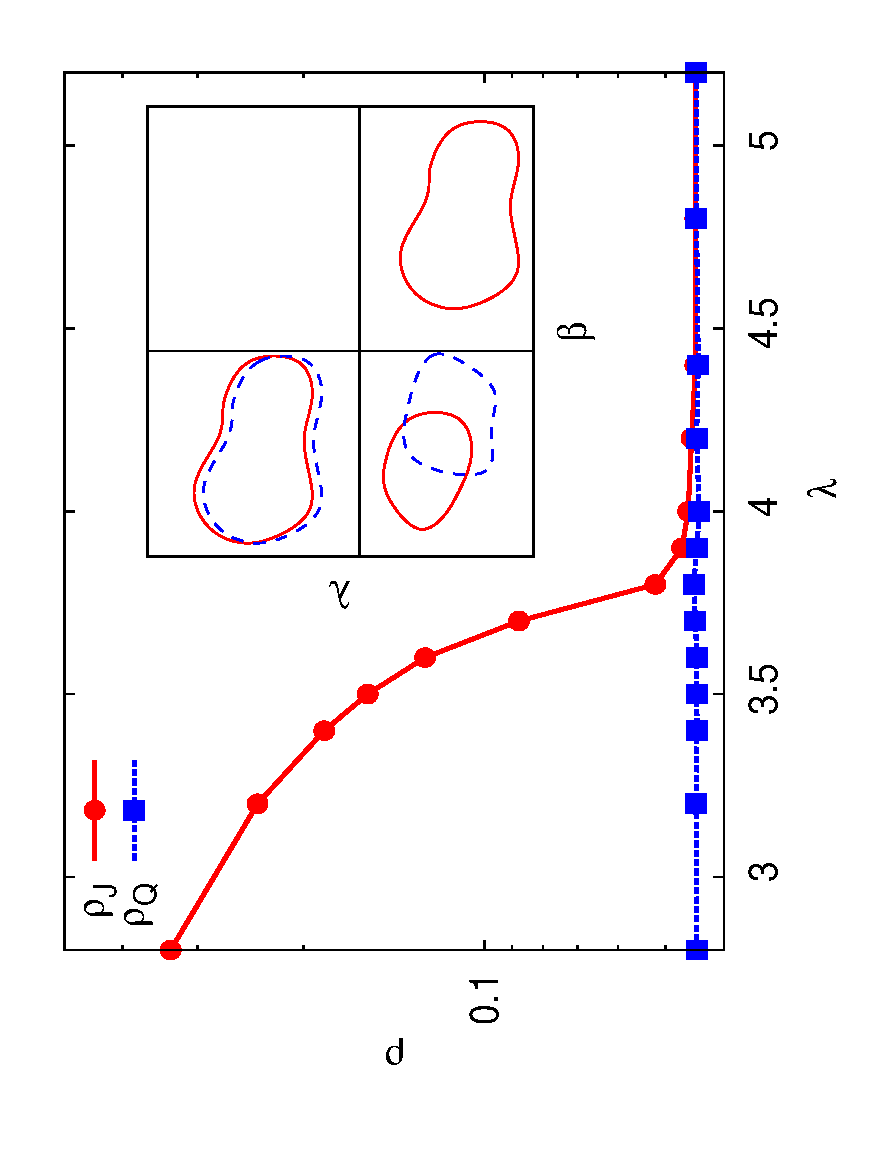
\includegraphics[angle=-90,width=0.6\linewidth]{figures/heisbulkout.eps}
\caption{Inset: Bulk phase diagram for the model in Eqs.~(\ref{action})~and~(\ref{SHeis}) with bosons and Heisenberg spins. The phase diagram is mathematically equivalent to a system of decoupled currents and spins, hence the straight line boundaries. At $\lambda=0$, the system has a paramagnet-ferromagnet transition as $\beta$ is increased, while the bosons are superfluid throughout. As $\lambda$ is increased, the boson currents bind to the hedgehog currents. The loop pictures in the phases show a ``snapshot'' of the phase. Red solid loops mean that boson currents are proliferated in the phase, while blue dashed loops indicate proliferated hedgehog currents. The phase of interest is the ``binding'' phase in the upper left corner where bosons are bound to hedgehogs. The main figure shows the current-current correlations of the bosons and hedgehogs as $\lambda$ is increased while $\beta=0$, for a system of linear dimension $L=6$. We see that the correlators become essentially equal as the system enters the upper left phase, indicating that bosons have bound to hedgehogs.}
\label{heisbulk}
\end{figure}


It is also helpful to think about the ``easy-plane'' regime for the spin variables, in which the spins, $\vec{n} = (n_a, n_b, n_c)$, are roughly in the $ab$-plane, with only small $c$ components; we will denote the corresponding global symmetry of spin rotations in the $ab$-plane as $U(1)_{\rm spin}$. In the easy-plane case we can define ``vortices'' of the XY spins $(n_a, n_b)$ (i.e., phase windings of the complex order parameter $\sim n_a + i n_b$). %which are the $ab$-components of the $\vec n$ variables. 
The vortices are defined on the plackets of the cubic lattice. Therefore in the (3+1)D space-time they are represented as two-dimensional ``world-sheets.'' When dealing with vortices, one can gain intuition by thinking in terms of only the three spatial dimensions of our (3+1) dimensional space-time. In this picture the bosons and hedgehogs are represented by point particles, while the vortices are represented by lines. The next two paragraphs can be most easily understood by thinking in this picture.

Though ordinary XY spins are not defined at the core of a vortex, our spins have a $c$-component which can point either up or down at the vortex core. We can define two species of vortices, which we call the $\uparrow$ and $\downarrow$ species, depending on whether $n_c$ is positive or negative at the core. This description is useful since an $\uparrow$ vortex ending and continuing as a $\downarrow$ vortex is a hedgehog. Therefore our system can be thought of as a system of vortex lines having two different species. These vortex lines can change species, and the locations where this happens are hedgehogs.\cite{LesikSenthil} This is illustrated in Fig.~\ref{monopoles}.

Hedgehog number can be either positive or negative, and this is determined by the properties of the vortex line the hedgehog is attached to.
If, when looking along the line from the $\uparrow$ core to the $\downarrow$ core the vorticity is clockwise (counterclockwise), we define a positive (negative) hedgehog.  This is pictured in Fig.~\ref{monopoles}.


\begin{figure}
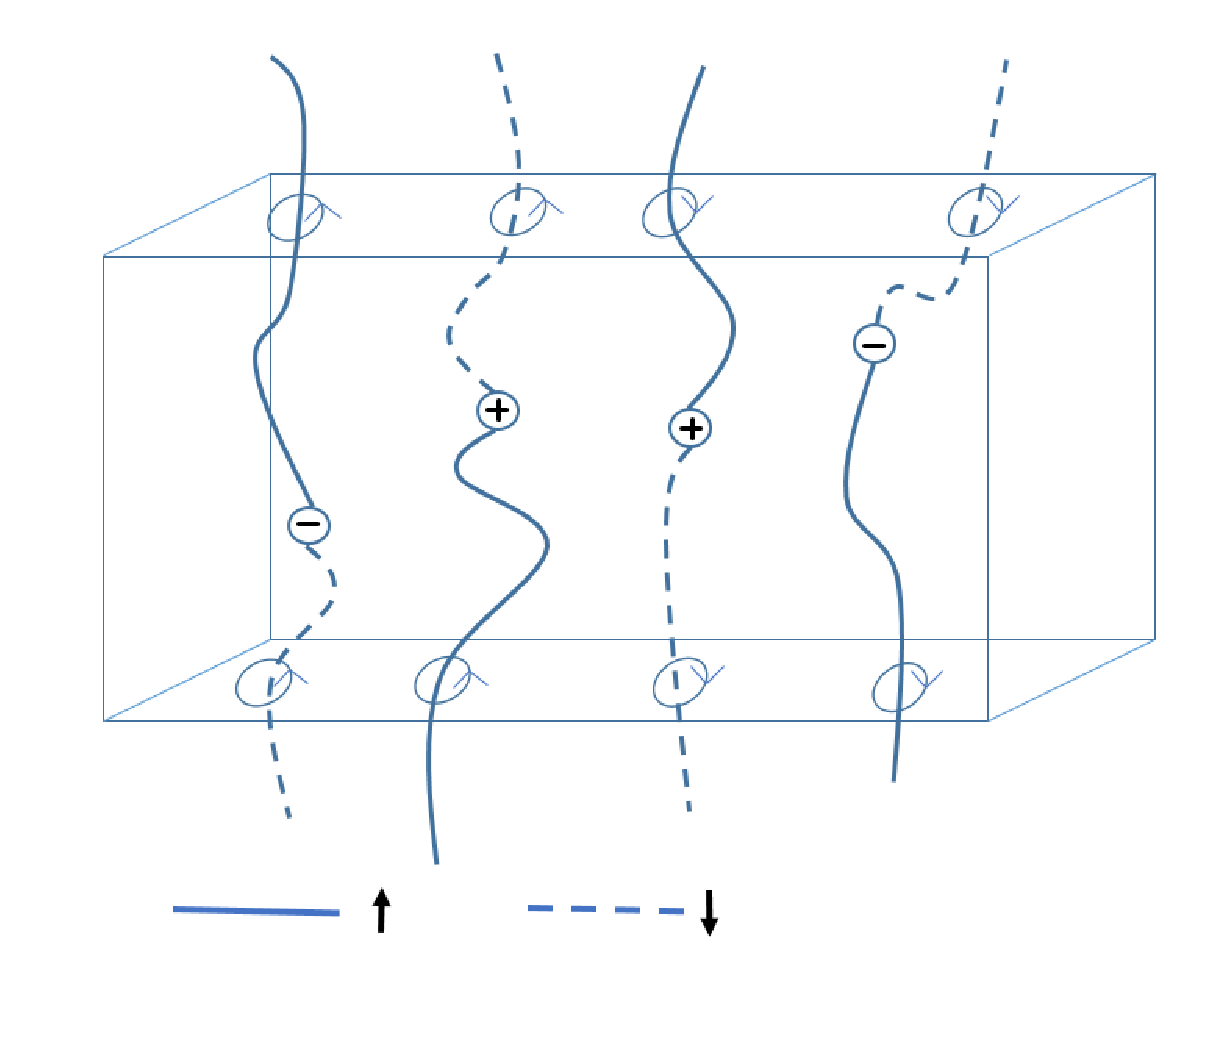
\includegraphics[width=0.6\linewidth]{figures/monopoles.eps}
\caption{As discussed in the text, the easy-plane spin system has two species of vortex lines, $\uparrow$ and $\downarrow$, depending on $n_c$ at the core. A hedgehog is a transition point between the two types of lines, with the sign of the hedgehog determined by the orientation of the type and vorticity of the vortex lines, as shown with examples. This figure shows only the spatial dimensions of the system, therefore the hedgehogs are point particles and the vortices are lines. Applying a Zeeman field to the surface means allowing only one type of vortex line through the surface. This leads to a correlation between the hedgehog number (and therefore the boson charge) and the vorticity at the surface, which is the origin of the Hall conductivity.}
\label{monopoles}
\end{figure}


%%%%%%%%%%%%%%%%%%%%%%%%%%%%%%%%%%%%%%%%%%%%%%%%%%%%%%%%%%%%%%%%%%%5
\subsubsection{Importance of Discrete Symmetry}
\label{subsubsec:HeisSym}

The action in Eq.~(\ref{action}) has a $U(1)$ symmetry which comes from the conservation of the $J_\mu$ currents; this is boson charge conservation symmetry. It also has an $SO(3)$ symmetry from the spins. Both of these symmetries participate in the protection of the topological phase, in the sense that if they are broken it is possible to continuously connect the topological phase to a trivial phase.
In addition, the action has a $\ztwo$ symmetry, which is obtained by reflecting the $\vec{n}$ spins in a plane in the spin space. To see how this affects the hedgehog current, we can examine Eq.~(\ref{alpha}), taking the reference vector $\vec{N}_0$ to be in the plane of reflection. We see that reflecting the spins changes the sign of the imaginary part of $e^{i\alpha_\mu}$, and therefore the hedgehog current changes sign under such a reflection. For our entire action to be invariant, we therefore need to combine such reflections with an operation which changes the sign of the boson currents. For concreteness we will consider the $\ztwo$ symmetry corresponding to reflections of the $\vec{n}$ variables in the $ab$ plane of the spin space. In this case the $\ztwo$ symmetry can be summarized as:
\begin{equation}
\begin{array}{ccc}
n_a,n_b & \rightarrow & n_a,n_b \\
n_c & \rightarrow & -n_c\\
Q_\mu & \rightarrow & -Q_\mu\\
J_\mu & \rightarrow & -J_\mu 
\end{array}.
\label{ztwoeqn}
\end{equation}
Note that it is also possible to reflect the $\vec n$ spins around a different plane, but this is not a distinct symmetry since it is simply the product of the above $\ztwo$ symmetry and an element of $SO(3)$. 

By analogy with the electronic topological insulator, we would like the $\ztwo$ symmetry described above to be a ``time-reversal'' symmetry, i.e.~it should be anti-unitary. The symmetry in Eq.~(\ref{ztwoeqn}) can be either a unitary or anti-unitary symmetry. Note that Eq.~(\ref{action}) is a real, (3+1)-dimensional action which is assumed to arise from the Trotter decomposition of the imaginary time propagator (i.e., Euclidean path integral) of a three-dimensional quantum Hamiltonian. The symmetry operations in Eq.~(\ref{ztwoeqn}) can be derived from the action of a symmetry operation on the quantum Hamiltonian. Therefore asking whether the symmetry in Eq.~(\ref{ztwoeqn}) is anti-unitary is the same as asking whether the symmetry of the quantum Hamiltonian which generates Eq.~(\ref{ztwoeqn}) is anti-unitary. This is a difficult question for us to answer as we do not know the quantum Hamiltonian which has Eq.~(\ref{action}) as its Euclidean path integral.  Nevertheless, we take the perspective where we can check whether the original Hamiltonian has time reversal by complex-conjugating the action combined with the appropriate variable transformations, and in this way we can view the above symmetry of the action also as time reversal.

In the easy plane case, our system has $U(1)_{\rm boson}\times U(1)_{\rm spin}$ in addition to this discrete symmetry. We can think of the $U(1)_{\rm spin}$ as also coming from a boson, and $n_a+i n_b$ gives the phase degree of freedom of this boson. We can imagine allowing tunnelling between the two $U(1)$ symmetries. If we do this, then the discrete symmetry should act the same way on the two species, and we can see that the above symmetry changes the number of the bosons but not their phase. In a system consisting of one species of bosons, the symmetry which acts in this way is anti-unitary.
From now on the symmetry described above will also be treated as anti-unitary and denoted by $\ztwot$.

The action in Eq.~(\ref{action}) is invariant under several $\ztwo$ symmetries, but for our purposes we will consider only the $\ztwot$ symmetry described above as important, as it protects the topological behavior. To see this we can break this symmetry and argue that the topological phase is destroyed.
We break the $\ztwot$ symmetry by introducing a Zeeman field into our action:
\begin{equation}
S_{\rm Zeeman}=-h\sum_R n_c(R).
\label{Zeeman}
\end{equation}
Here $h$ is the strength of the Zeeman field, which points in the $c$-direction. Note that the Zeeman field does not break $U(1)_{\rm spin}$ or $U(1)_{\rm boson}$. In our picture of two species of vortices (Fig.~\ref{monopoles}), the Zeeman field forbids one of the species. Since the vortex lines cannot change species, hedgehogs are forbidden and the binding phase is destroyed. 
This can be made more precise if we replace the binding term in Eq.~(\ref{action}) with the following term:
\begin{equation}
\frac{\lambda}{2}\sum_{r,\mu} [ J_\mu(r) - \eta Q_\mu(r)]^2 ~,
\label{tbind}
\end{equation}
where $\eta$ is a real number. If we choose the parameters $\beta$ and $\lambda$ so that the system is initially in the binding phase, the introduction of $\eta$ allows us to tune the system between the binding phase ($\eta=1$) and the trivial insulator ($\eta=0$). Without a Zeeman field, the system undergoes a phase transition as $\eta$ is changed between $1$ and $0$. 
When a Zeeman field is applied, the hedgehogs are effectively forbidden, and so we can tune parameters $h$ and $\eta$ without going through a phase transition. Indeed, when $\eta=1$, the change of variables in Eq.~(\ref{shift}) leads to decoupled $\tilde{J}$ currents and spins, so there is no phase transition when making $h$ arbitrarily large to align all spins. We can then tune $\eta$ to zero and finally reduce $h$ back to zero, all without undergoing a phase transition.  Thus, in the presence of the Zeeman field, the phase with $\eta=1$ is not distinct from the trivial insulator.


%%%%%%%%%%%%%%%%%%%%%%%%%%%%%%%%%%%%%%%%%%%%%%%%%%%%%%%%%%%%%%%%%%%
\subsubsection{Binding of Multiple Bosons to a Hedgehog}
The above methods also allow us to answer the question of what happens to the system if $\eta$ in Eq.~(\ref{tbind}) is an integer larger than 1.  In a $U(1)\times U(1)$ system in two dimensions, we studied the binding of multiple bosons to vortices (realized by taking integer $\eta$) and found that each number of bound bosons led to a different symmetry-protected topological phase.\cite{FQHE} There were therefore as many SPTs as there are integers, in agreement with the cohomology classification.\cite{WenScience,WenPRB, LuVishwanath} In the present three-dimensional case the classification of Chen et al.\cite{WenScience,WenPRB} for $U(1)$ and $\ztwot$ symmetry predicts the existence of only a finite number of such symmetry protected topological phases, implying that not every value of $\eta$ would lead to a distinct phase. Indeed, we find that all systems with $\eta$ an even integer are topologically trivial, while when $\eta$ is odd we have the same topological phase as $\eta=1$. 

We can justify this claim by showing that $\eta=2$ can be continuously connected to $\eta=0$ which is a trivial insulator. This argument can then be extended to show that any two systems where $\eta$ differs by $2$ are in the same phase.  Our argument is inspired by Ref.~\cite{BiRasmussenXu13}, except that here we are working with a microscopic model rather than a topological field theory.
We start by considering two copies of our action, each with its own bosons and Heisenberg spins and with $\eta=1$:
\begin{eqnarray}
&&S=-\beta\sum_{R,\mu}\left[ \vec{n}^{(1)}(R)\cdot \vec{n}^{(1)}(R+\hat{\mu})+\vec{n}^{(2)}(R)\cdot \vec{n}^{(2)}(R+\hat{\mu})\right]\nonumber\\
&&+\frac{\lambda}{2}\sum_{r,\mu}\left( [ J_\mu^{(1)}(r)- Q_\mu^{(1)}(r)]^2+[ J_\mu^{(2)}(r)- Q_\mu^{(2)}(r)]^2\right),
\label{doubleaction}
\end{eqnarray}
where the superscripts indicate which copy a variable is from.  We now couple the two copies by adding the following terms:
\begin{eqnarray}
\delta S=-A\sum_{R} \vec{n}^{(1)}(R)\cdot \vec{n}^{(2)}(R)
-B\sum_{r} \cos[\Phi^{(1)}(r)-\Phi^{(2)}(r)].
\label{AB}
\end{eqnarray} 
When $A$ is large and positive, the first term above locks spins of the different copies together, $\vec{n}^{(1)}\approx\vec{n}^{(2)}$. The hedgehog variables therefore take on the same values, and either can be viewed as the hedgehog number of the whole spin system in this case: $Q \approx Q^{(1)} \approx Q^{(2)}$. On the other hand, when $A$ is large and negative the spins of different types are locked in opposite directions,  $\vec{n}^{(1)}\approx -\vec{n}^{(2)}$, and $Q^{(1)} \approx -Q^{(2)}$.

The $\Phi$ variables are $2\pi$-periodic phases that can be thought of as conjugates to the $J_\mu$ variables. More precisely, in our path integral we sum over only the configurations of $J_\mu$ in which the currents are divergenceless. We can instead sum over all configurations of $J_\mu$, and include the following term in our path integral:
\begin{equation}
\int_0^{2\pi} D\Phi(r) e^{-i\sum_r \Phi(r)(\sum_\mu\nabla_\mu J_\mu)(r)} ~,
\end{equation}
which dynamically enforces the constraint that the boson currents be conserved. We introduce $\Phi$ variables for each copy of the boson currents, and the $B$ term is tunnelling between the two copies. 
When $B$ is large (of either sign) only the sum of $J^{(1)}$ and $J^{(2)}$ is conserved and can be identified as the current of the whole boson system (i.e., combining both copies).

When $A$ and $B$ are large and positive, we can expand the terms on the second line of Eq.~(\ref{doubleaction}), and take $J = J^{(1)} + J^{(2)}$, $Q = Q^{(1)} = Q^{(2)}$. In this case we obtain coupling between $J$ and $Q$ which is effectively the same as in Eq.~(\ref{tbind}) with $\eta=2$. 
On the other hand, when $A$ is large and negative, but $B$ is still large and positive, $J$ is unchanged but its coupling to the hedgehogs vanishes as contributions from $Q^{(1)}$ and $Q^{(2)}$ cancel; this gives Eq.~(\ref{tbind}) with $\eta=0$.
We can continuously deform $A=0$, $B=0$ to $A=\infty$, $B=\infty$ without undergoing a phase transition. In addition, we can deform $A=0$, $B=0$ to $A=-\infty$, $B=\infty$ without undergoing a phase transition. This implies that we can tune from $\eta=2$ to $\eta=0$ without undergoing a phase transition, and so both of these cases are in the trivial insulating phase.


%%%%%%%%%%%%%%%%%%%%%%%%%%%%%%%%%%%%%%%%%%%%%%%%%%%%%%%%%%%%%%%%%5
\subsection{Phase Diagram on the Boundary Between the Binding Phase and a Trivial Insulator}
\label{subsec:heissurf}
By analogy to the fermionic topological insulator, we expect that one way to investigate the topological nature of our phase is to study the physics of its surface. In particular, a number of interesting phases have been predicted on the surface of the bosonic TI,\cite{SenthilVishwanath} and if we can identify these phases on the surface of our binding phase, it will be a powerful argument that the binding phase is a bosonic TI.

We introduce a surface between the binding phase and a trivial insulator by allowing $\eta$ in Eq.~(\ref{tbind}) to vary spatially.
We vary $\eta$ in the $z$ direction, so that:
\begin{equation}
\eta[r=(x,y,z,\tau)]=
\left\{ \begin{array}{cc}
1, &~ z_L\leq z<z_R\\
0, &~ \rm{otherwise}\\
\end{array}\right..
\label{eta_r}
\end{equation}
This leads to the binding phase in the region $z_L < z < z_R$, while the trivial phase occupies the rest of the space. Note that there are two surfaces of the binding phase: one at $z_L$ and one at $z_R$. The above geometry in our Monte Carlo setup with periodic boundary conditions corresponds to a four-dimensional torus which is divided into two parts along the $z$-direction.

On the surface, we can measure all of the quantities which we measured in the bulk, but we now only sum over the sites near the surface (and when averaging over directions we only use the $\hat{x}$, $\hat{y}$ and $\hat{\tau}$ directions). 

The binding between hedgehogs and bosons in the bulk of the topological phase leads to exotic physics on the surface. In both the binding and trivial phases, hedgehog currents are proliferated, while boson currents are bound to the hedgehog currents in the binding phase and are absent in the trivial phase, as shown in Fig.~\ref{surface}. Consider what happens when a hedgehog loop tries to cross the boundary between the phases. Since the boson currents must form closed loops, the above conditions cannot both be satisfied without something interesting happening on the surface. For example, we could have unbound boson currents on the surface, or hedgehogs could be effectively forbidden from crossing the surface.


\begin{figure}
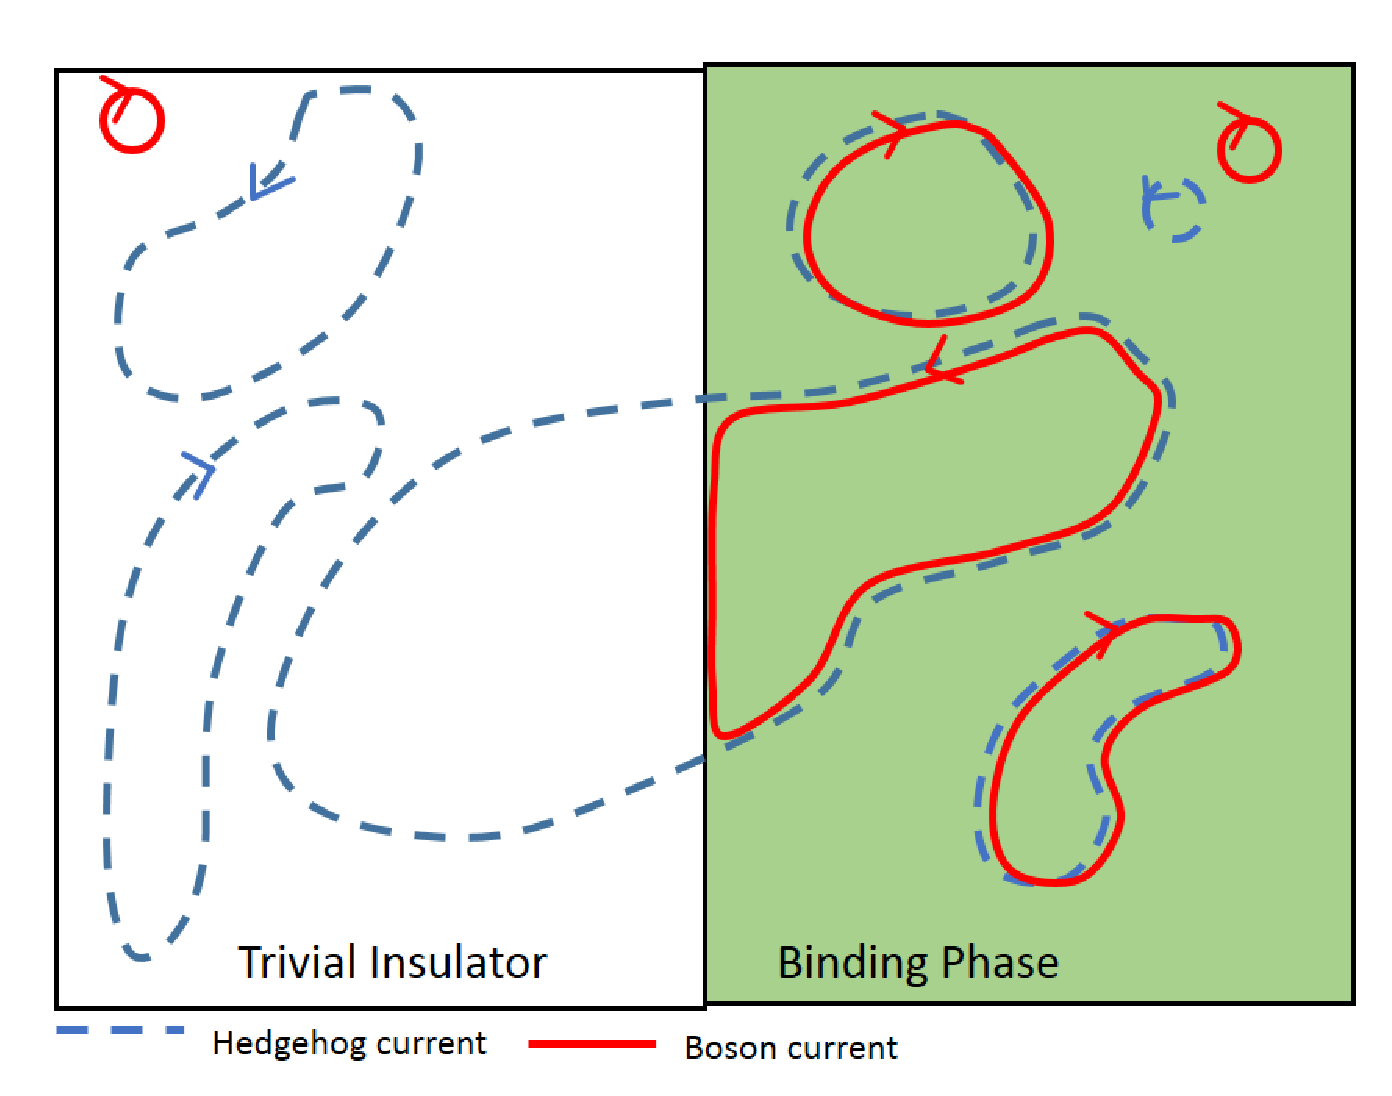
\includegraphics[width=0.6\linewidth]{figures/surface.eps}
\caption{A snapshot of the system, when it is spatially divided into a region which is a trivial insulator and a region which is in the binding phase. In the trivial phase, boson currents are gapped and hedgehog currents are proliferated. In the binding phase both currents are gapped individually, but their bound states are proliferated. Large hedgehog current loops can exist in either region; however, when such a loop tries to cross the boundary the conservation of boson current leads to a conflict between the two sides, and this can lead to exotic surface physics. }
\label{surface}
\end{figure}


In order to study the surface physics and search for the exotic surface behavior predicted in Ref.~\cite{SenthilVishwanath}, we first determine the surface phase diagram.
To do this, we fix the values of $\beta$ and $\lambda$ in the bulk and tune them only on one of the surfaces, by setting:
\begin{eqnarray}
\beta_\mu(X,Y,Z,T) &=&
\left\{
\begin{array}{ll}
\beta_{\rm surf}, & Z = z_R - 1/2, ~\mu=\hat{x},\hat{y},\hat{\tau}\\
\beta_{\rm bulk}, & {\rm otherwise}
\end{array}\right. ~
\label{bulkvsurf} \\
\lambda_\mu(x,y,z,\tau) &=&
\left\{
\begin{array}{ll}
\lambda_{\rm surf}, & z = z_R, ~\mu=\hat{x},\hat{y},\hat{\tau}\\
\lambda_{\rm bulk}, & {\rm otherwise }
\end{array}\right. ~.
\end{eqnarray}
Here we focused on the surface at $z_R$, and $\mu$ denotes link orientation for either $\beta$ or $\lambda$ terms.  We show the surface phase diagram in the inset of Fig.~\ref{heissurf}.  All data was taken with $\beta_{\rm bulk}=0$, $\lambda_{\rm bulk}=5.2$, parameters which put the bulk deep into the binding phase.  The surface phase diagram contains three distinct phases. When $\lambda_{\rm surf}$ is small the bosons are in a superfluid phase, breaking their $U(1)$ symmetry. This is the scenario pictured in Fig.~\ref{surface}, where hedgehogs can cross the surface, and these crossings are connected by boson currents. If $\beta_{\rm surf}$ is also small the $SO(3)$ symmetry is unbroken as the spins are disordered. As $\beta_{\rm surf}$ increases at small $\lambda_{\rm surf}$, the $SO(3)$ symmetry breaks, and so both symmetries are broken. Finally, at large $\lambda_{\rm surf}$ bosons see a large energy cost, and so the $U(1)$ symmetry is unbroken. This forbids hedgehogs from crossing the surface, leading to a system of $SO(3)$ spins with hedgehogs forbidden, which on the three-dimensional cubic latice is known to have magnetic order thus breaking the $SO(3)$ symmetry.\cite{LauDasgupta, LesikAshvin} 


\begin{figure}
\includegraphics[angle=-90,width=0.6\linewidth]{figures/heissurf.eps}
\caption{The inset shows the phase diagram of the surface of the binding phase, without a Zeeman field. It was obtained by tuning the bulk parameters deep into the binding phase and then varying $\beta$ and $\lambda$ {\em only on the surface}.  We find that in this model our surface always spontaneously breaks a symmetry. At small $\beta_{\rm surf}$ and $\lambda_{\rm surf}$ the boson $U(1)$ symmetry is broken and the bosons condense into a superfluid, while at large $\lambda_{\rm surf}$ the spin $SO(3)$ symmetry is broken and the spins align into a ferromagnet. At small $\lambda_{\rm surf}$ and large $\beta_{\rm surf}$ both symmetries are broken.  The main plot shows surface magnetization on a sweep in $\lambda_{\rm surf}$ for $\beta_{\rm surf}=0$. We show $mL^{3/2}$, which is independent of system size in the disordered phase, and grows with system size in the ordered phase. We can clearly see that the $SO(3)$ symmetry is broken as $\lambda_{\rm surf}$ is increased past a value of approximately $4$. All data in this section was taken with $\beta_{\rm bulk}=0$, $\lambda_{\rm bulk}=5.2$.}
\label{heissurf}
\end{figure}


The locations of the phases and phase transitions in Fig.~\ref{heissurf} were determined by studying singularities in the specific heat, as well as by studying the surface magnetization and current-current correlators. As an example of such data, in the main plot of Fig.~\ref{heissurf} we show the magnetization, multiplied by the square-root of the volume of the surface ($L^{3/2}$). This quantity should be constant when the spins are disordered and should grow with system size when they are ordered. The data was taken with $\beta_{\rm surf}=0$ and increasing $\lambda_{\rm surf}$. We can see that the spins order at $\lambda_{\rm surf} \approx 4$. 

In order to use the current-current correlators to detect the breaking of the $U(1)$ boson symmetry on the surface, we must think through such measurements carefully.  In a $D$-dimensional system of boson worldlines (space-time currents), the argument that $\rho_J(k_{\rm min}) \sim k_{\rm min}^2 \sim 1/L^2$ in the gapped phase relies on the conservation of the currents $J$.  However, this is no longer true if we consider only the surface, as currents can enter and exit from the rest of the system.  
Therefore we instead measure the current-current correlators in the entire system (though only in the $\hat{x}$, $\hat{y}$, and $\hat{\tau}$ directions, which are parallel to the surface). When currents are gapped everywhere, this quantity will still be proportional to $1/L^2$. 
If we measured the current-current correlator only on the surface in the phase where the surface is a superfluid, we would expect the result to be independent of system size. Since we are measuring the correlator over the whole system, the result should be proportional to the fraction of the system which makes up the surface, which is $1/L$.
In Fig.~\ref{slabcurs} we plot $\rho_J \cdot L^2$. We see that at large $\lambda_{\rm surf}$ this quantity is independent of system size, which tells us that the currents are gapped everywhere and the surface is an insulator in the boson degrees of freedom. At small $\lambda_{\rm surf}$, $\rho_J\cdot L^2 \sim L$, which tells us that there is a region whose volume fraction is proportional to $1/L$ where the bosons are in a superfluid phase. We interpret this as evidence that there is a superfluid at the surface.


\begin{figure}
\includegraphics[angle=-90,width=0.6\linewidth]{figures/slabcurs.eps}
\caption{Current-current correlators of the entire system, multiplied by $L^2$, used to detect symmetry breaking of the bosons on the surface. This quantity is constant when the boson $U(1)$ symmetry is preserved and increases linearly with system size when it is broken on the surface. Parameters used are the same as in Fig.~\ref{heissurf}. We see that there is a phase transition at $\lambda_{\rm surf}\approx 4$.
}
\label{slabcurs}
\end{figure} 


The surface phase where the $U(1)$ boson symmetry is broken is clearly a superfluid of bosons. In the easy-plane picture the spins can also be thought of as having a $U(1)$ symmetry which is broken when the spins are ordered, and so the phase where the spins order can also be thought of as a superfluid of new particles representing the spins. We can now ask whether these superfluids are trivial superfluids, or the exotic superfluids thought to exist on the surface of a bosonic TI.\cite{SenthilVishwanath} The exotic properties have to do with the charge and statistics of gapped vortex excitations, and unfortunately we do not have access to these properties in our Monte Carlo. Therefore our surface superfluids cannot tell us whether the binding phase is a bosonic TI.

One predicted feature of the superfluids on the surface of the bosonic TI is that they are connected by a direct transition which is a deconfined critical point.\cite{SenthilVishwanath} As shown in Figs.~\ref{heissurf} and \ref{slabcurs}, our $SO(3)$ and $U(1)$ symmetries appear to break on the opposite sides of the same point, and so it looks that we also have a direct transition between these phases; however, we would need larger system sizes to see whether there is indeed a direct transition and whether it is continuous.
Though this does not definitively show that the binding phase is topological, but it does provide evidence that we have an unusual field theory on the surface.


\subsection{Surface with Zeeman Field}
Another exotic phase predicted to exist on the surface of the bosonic TI is a phase which breaks $\ztwot$ symmetry and has a quantized Hall reponse. We can try to realize this phase by applying a Zeeman field on the surface of our model to explicitly break the $\ztwot$ symmetry. We add a term similar to Eq.~(\ref{Zeeman}) to our action, but only on the surface of the model. We then expect that there is a surface phase which does not break any $U(1)$ symmetry---i.e., an insulator---but which has the surface Hall conductivity quantized to an odd integer, which is different from the even values expected in the (2+1)D bosonic integer quantum Hall effect. For easy-plane spins, we expect that a finite Zeeman field is needed to destroy the surface superfluids to reach this phase, while for SO(3) spins used here and starting in the spin-ordered phase, we expect to immediately transition to the quantum Hall insulator.\cite{LesikAshvin}

In our Monte Carlo study, we actually apply Zeeman field $h$ to both surfaces but take the fields on the two surfaces to have opposite signs.  We take $\lambda=5.2$ and $\beta=0$ everywhere (including at the surfaces), which puts the bulk regions deep into the binding or trivial phases respectively, while the surfaces start in the spin-ordered phase at $h=0$.

Since the Hall conductivity in the surface system of spins and bosons will be due to correlations between the vorticity of the spins and the boson charges,\cite{FQHE} we will measure these correlations directly before moving on to the more complicated Hall conductivity measurement. 
In the absence of the Zeeman field, we can use the $\ztwot$ symmetry, which is reflection of the $\vec n$ variables in the $ab$-plane, to change the sign of hedgehog and hence the boson charge without changing the spin vorticity, and so such correlations vanish. This can be seen in Fig.~\ref{monopoles}, where, for example, on the top surface there is one clockwise vortex attached to a positive hedgehog (which is in turn bound to a positively charged boson), and another clockwise vortex is attached to a negative hedgehog. Applying a Zeeman field corresponds to only allowing one type of vortex ($\uparrow$ or $\downarrow$) to pass through the surface. In Fig.~\ref{monopoles}, this means that only solid lines are allowed to pass through the top surface. We can see that this leads to a correlation between the vorticity of the vortex on the surface and the charge of the boson it is binding nearby. 

We can further think about Fig.~\ref{monopoles} as depicting a slab of the binding phase. Opposite Zeeman fields on the two surfaces give us a quasi-two-dimensional slab on which vortices are bound to charges with definite relation between the vorticity and charge, and these bound states are proliferated. We have studied such a system in a previous work,\cite{FQHE} and found that its Hall conductivity is quantized to be equal to two. It is reasonable to assume that this conductivity is evenly distributed between the two surfaces, leading to the surface Hall conductivity equal to one on each surface. This intuitive argument reproduces the prediction of Ref.~\cite{SenthilVishwanath}.

To measure correlations between vortices and bosons we first define the spin vorticity $V_{\mu\nu}(R)$ as
\begin{equation}
V_{\mu\nu}(R) = \frac{1}{2\pi}[\nabla_\mu s_{\nu}(R) - \nabla_\nu s_{\mu}(R)] ~,
\label{Vmn}
\end{equation}
where $s_\mu(R) \in (-\pi, \pi]$ measures the difference between the spin angles at $R+\hat{\mu}$ and $R$ and brings it to $(-\pi,\pi]$:
\begin{equation}
s_{\mu}(R)\equiv \left[\tan^{-1}\left(\frac{n_b(R+\hat{\mu})}{n_a(R+\hat{\mu})}\right) -\tan^{-1}\left(\frac{n_b(R)}{n_a(R)}\right)\right]{\rm mod}~2\pi.\nonumber
\end{equation}
We can then Fourier transform the vorticity as follows:
\begin{equation}
V_{xy}(k) = \frac{1}{\sqrt{L^3}}{\sum_{R}}^\prime V_{xy}(R) e^{-ik\cdot R}.
\end{equation}
The prime on the sum indicates we are summing over all sites at a fixed $z=z_R$. We measure $\left|\la V_{xy}(k_{\rm min})J_\tau(-k_{\rm min})\ra\right|$, where $k_{\rm min}=(2\pi/L,0,0,0)$, and the results are shown in Fig.~\ref{heishall}. 

We see that as soon as the Zeeman field is applied, the vortices and charges become correlated. Unlike the Hall conductivity, we do not expect these correlations to approach any universal value. We do note that the correlations on the two surfaces of the system are approximately equal, which is encouraging as we would expect the Hall conductivity on these surfaces to be equal as well. The differences between the correlations on the two surfaces is likely due to the fact that the surfaces are realized differently on a lattice, but we would expect that universal values such as the Hall conductivity would not have these differences.

In order to measure Hall conductivity, we need to couple both the bosons and spins to external probing gauge fields, and then use linear response theory to determine the conductivity. When we do this we run into a problem, which has to do with the way the hedgehog currents $Q_\mu$ were defined. We can see from Eq.~(\ref{omega}) that $\omega_{\mu\nu}$ is a discontinuous function of spins since we required it to be brought to $(-\pi, \pi]$. When including the probing gauge fields, this causes the path integral to be a discontinuous function of the probing fields, which prevents us from taking the derivatives needed for linear response theory, and so we do not know how to calculate conductivity in this system. In the next section we will find a way around this problem, while in the present case we can only appeal to the intuitive argument presented above.


\begin{figure}
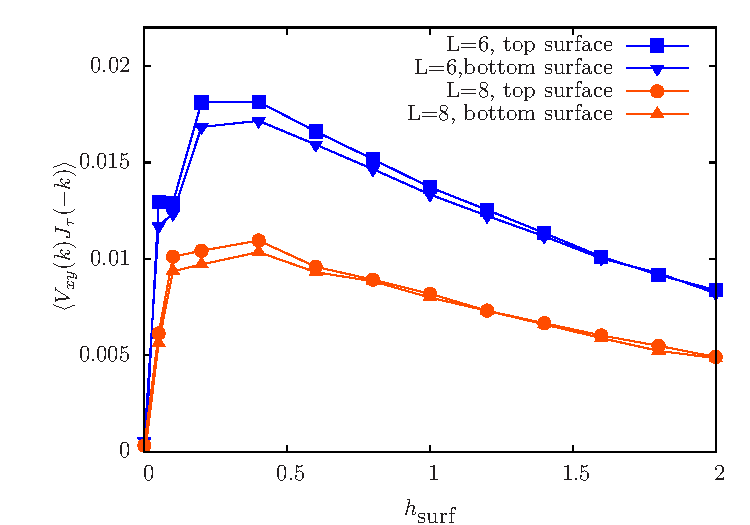
\includegraphics[width=0.6\linewidth]{figures/vortexcor.eps}
\caption{Spin vortex - boson charge correlators near the surface of the binding phase in the model Eqs.~(\ref{action})~and~(\ref{SHeis}) using Heisenberg spins. The horizontal axis is the strength of the Zeeman field applied only near the surfaces (and of opposite sign on the two surfaces). We see that as soon as the Zeeman field is turned on, the correlator takes a non-zero value. The value is non-universal, but is approximately the same on the top and bottom surfaces. Data was taken with $\beta=0$, $\lambda=5.2$ everywhere and the binding phase occupying half of the system, cf.\ Eq.~(\ref{eta_r}).  Since we do not know how to properly couple external gauge fields to this system, we are unable to compute the Hall conductivity.
}
\label{heishall}
\end{figure}



%%%%%%%%%%%%%%%%%%%%%%%%%%%%%%%%%%%%%%%%%%%%%%%%%%%%%%%%%%%%%%%%%%%%%%%%%%%%%%%%%%%%%%%%%%%%%%%5

\section{Realizing the topological insulator by binding bosons to hedgehogs of an easy-plane \cp model}
\label{section::CP1}

The Heisenberg model discussed in the previous section allowed us to realize a ``binding'' phase of bosons and hedgehogs. However, in this model we were unable to find definitive evidence that the binding phase is in fact a symmetry-protected bosonic topological insulator, although our indirect arguments are compelling. In this section we introduce a new model, which includes the spin degrees of freedom in a \cp representation. 
This theory has spinor matter fields (``spinons'') coupled to a compact gauge field and is a faithful representation of the microscopic spin system with short-range interactions (i.e., such a lattice ``field theory'' is ``emergable'' from a local microscopic Hamiltonian). We will see that this formulation allows us to make measurements, such as a Witten effect in the bulk and a quantized Hall conductivity on the surface, which indicate that the binding phase is a bosonic TI.

\subsection{Bulk Phase Diagram}
The following action represents the spins in the $CP^1$ representation:
\begin{eqnarray}
S_{\rm spin}=-\beta\sum_{s=\uparrow,\downarrow}\sum_{R,\mu} [z_s^\dagger(R)z_s(R+\hat\mu)e^{-ia_\mu(R)}+c.c.] 
-K\sum_{R,\mu<\nu} \cos[\nabla_\mu a_\nu(R)-\nabla_\nu a_\mu(R)].
\label{cp1action}
\end{eqnarray} 
Here the spins are represented by two complex bosonic fields $z_\uparrow$,$z_\downarrow$ (``spinons''), which satisfy $|z_\uparrow|^2+|z_\downarrow|^2=1$. We can write the $z$ fields as a spinor, $\mathbf{z}\equiv(z_\uparrow,z_\downarrow)^T$, and extract the spin $\vec{n}=\mathbf{z^\dagger} \vec\sigma \mathbf{z}$, where $\vec{\sigma}\equiv (\sigma_1,\sigma_2,\sigma_3)$ is a vector of Pauli matrices.
The spinon fields are minimally coupled to a compact gauge field $a_\mu(R)$. The last term is a Maxwell-like term for the compact gauge field, which appears after partially integrating out the spinon fields. The variables in the above action live on a cubic lattice, where $R$ gives the position on the lattice and $\mu$,~$\nu$ are directions.

The \cp model defined above actually has global $SO(3)$ symmetry, similar to the previous section. In this section we find it convenient to break the $SO(3)$ symmetry down to $U(1)$ explicitly by taking the ``easy-plane'' limit of the $CP^1$ model. We align all the spins $\vec{n}$ in the $ab$-plane, which corresponds to fixing the magnitude of $z_\uparrow$ and $z_\downarrow$, and allowing only phase fluctuations, i.e., $z_s\equiv \frac{1}{\sqrt{2}}e^{i\phi_s}$. The $CP^1$ model in the easy-plane limit becomes:
\begin{eqnarray}
S_{\rm spin}=-\beta\sum_{s=\uparrow,\downarrow}\sum_{R,\mu} \cos[\nabla_\mu\phi_s(R)-a_\mu(R)]
+\frac{K}{2}\sum_{R,\mu<\nu}\left[\nabla_\mu a_\nu(R)-\nabla_\nu a_\mu(R)-2\pi B_{\mu\nu}(R)\right]^2.
\label{sspin}
\end{eqnarray}
Here $\phi_\uparrow$ and $\phi_\downarrow$ are $2\pi$-periodic variables which represent the phases of the spinon fields. We have also replaced the cosine in the Maxwell term by a quadratic ``Villain'' form, with $B_{\mu\nu}$ which are unconstrained, integer-valued dynamical variables residing on the plackets of the lattice. Upon summing over $B_{\mu\nu}$ in the partition sum, the third term generates a $2\pi$ periodic function of $\nabla_\mu a_{\nu}-\nabla_\nu a_{\mu}$, and therefore this does not change the universality class of the problem.

Using the Villain form of the Maxwell term is advantageous as it allows us to define the hedgehog current:
\begin{equation}
Q_\mu(r)=\frac{1}{2}\epsilon_{\mu\nu\rho\sigma}\nabla_\nu B_{\rho\sigma}.
\label{mondef}
\end{equation}
Note that $Q_\mu(r)$ resides on the links of the lattice whose sites are labelled by $r$ which, as in the previous section, is interpenetrating with the lattice labelled by $R$. The above definition is analogous to Eq.~(\ref{monopoledef}) with $B_{\rho\sigma} \leftrightarrow \omega_{\rho\sigma}/(2\pi)$. The $B_{\mu\nu}$ variables have the meaning of ``Dirac strings'' of the hedgehogs. Thus defined, the hedgehogs in the \cp model are actually monopoles of the compact gauge field $a_\mu$. We will continue to call them hedgehogs in this work to avoid confusion with a different type of monopole introduced later. 

We can again study the model described by Eqs.~(\ref{action}) and (\ref{sspin}) in Monte Carlo. Equilibration becomes difficult in the regime where $K$ and $\lambda$ are large, and it is necessary to include composite updates which simultaneously change multiple variables. One such update is to change $B_{\mu\nu}$ while also changing $J_\mu$ so that there is no change in the second term in Eq.~(\ref{action}). Another update is to change both $a_\mu$ and $B_{\mu\nu}$ in such a way as to keep the $K$ term in Eq.~(\ref{sspin}) small. 

We can find phase transitions in this model by looking for singularities in the specific heat, which is defined in the same way as in the previous section. We can identify order in the bosonic degrees of freedom by studying the superfluid stiffness and order in the spins by studying the magnetization. In this easy-plane version of the model, the spin degree of freedom is an $XY$ vector with components $(n_a,n_b)$.  Since $(n_a, n_b) = (\cos\phi_{\rm spin}, \sin\phi_{\rm spin})$ with $\phi_{\rm spin} = \phi_\uparrow - \phi_\downarrow$, the magnetization is given by:
\begin{equation}
m = \frac{\left\langle\left|\sum_R e^{i [\phi_\uparrow(R) - \phi_\downarrow(R)]}\right|\right\rangle}{\rm Vol}. 
\label{cp1mag}
\end{equation}

The phase diagram in this model is parameterized by $\beta$, $K$, and $\lambda$. As in the previous section, we can make the change of variables in Eq.~(\ref{shift}) and find that the $\tilde{J}$ part of the problem decouples from the spin part. The behaviour of the bosons is the same as in the previous section. When $\lambda$ is small, the physical bosons are essentially independent of the hedgehogs, and are in the superfluid phase. As $\lambda$ is increased, they become bound to hedgehogs. The transition happens at $\lambda\approx 4$. 
The locations of the phase transitions in the spin degrees of freedom are independent of $\lambda$, though the nature of the various phases are not. In Fig.~\ref{cp1bulkphase} we show the phase diagram in the $\beta$ and $K$ variables, for two cases: $\lambda$ small and $\lambda$ large. The phase diagram is consistent with the easy-plane $CP^1$ model in the literature.\cite{artphoton} 

Let us first consider the case when $\lambda$ is small. The bosons will be in a superfluid phase for any $\beta$ and $K$. The spin system has the following three phases: 
{\it i)} When $\beta$ and $K$ are small, the spin degrees of freedom are disordered and the hedgehogs are proliferated. The phase is therefore a conventional paramagnet in the spin degrees of freedom. 
{\it ii)} As $K$ is increased, hedgehogs acquire a large energy cost, and become gapped. This phase was studied in Refs.~\cite{LesikSenthil, LesikAshvin, artphoton}. It is known as the Coulomb phase\cite{HermeleFisherBalents} because it has an emergent gapless photon and gapped excitations that carry charge $1/2$ and interact via a Coulomb interaction. 
{\it iii)} Finally, the phase at large $\beta$ has a large energy penalty for spin fluctuations, and so the spins order. This phase is a conventional ferromagnet in the spin degrees of freedom. 

In the case when $\lambda$ is large, the spin parts of the Coulomb and ferromagnetic phases do not change, since both of these phases suppress hedgehogs. These phases are now trivial insulators in the boson degrees of freedom. On the other hand, in the paramagnetic phase the hedgehogs are proliferated and the bosons become bound to them. This is the binding phase, which we will argue is a topological phase protected by the $U(1)_{\rm spin}\times U(1)_{\rm boson}$ and $\ztwot$ symmetries.



\begin{figure}
\includegraphics[angle=-90,width=0.6\linewidth]{figures/cp1bulkphase.eps}
\caption{Bulk phase diagram in the $\beta$ and $K$ variables for the model defined in Eqs.~(\ref{action}) and (\ref{sspin}) where the spins are described by an easy-plane $CP^1$ model. The top panel shows the phases at small $\lambda$, while the bottom panel shows large $\lambda$. The locations of the phase boundaries are independent of $\lambda$, but the nature of the phases are not. Symbols indicate points where the phase transitions were identified numerically from singularities in the heat capacity. The candidate for the topological phase is the binding phase, which occurs at large $\lambda$, small $\beta$, and small $K$. }
\label{cp1bulkphase}
\end{figure}
 

\subsubsection{Symmetries When The Spins Are Represented By An Easy-plane \cp Model}
When representing our spins with an easy-plane \cp model we have explicitly broken the $SO(3)$ symmetry from the previous section down to a $U(1)$ symmetry which corresponds to spin rotations in the easy plane. 
This complicates our discussion of the discrete symmetries of the model. In the previous section all reflections of $\vec{n}$ were related to each other by an operation in $SO(3)$, but in the easy-plane case, e.g., reflections in the $ab$ plane $(n_a, n_b, n_c) \to (n_a, n_b, -n_c)$ are now distinct from reflections in the $ac$ plane $(n_a, n_b, n_c) \to (n_a, -n_b, n_c)$. The result of this is that there are now two $\ztwot$ symmetries which protect the topological phase, in the sense that as long as any one of these symmetries is preserved, the topological phase cannot be continuously connected to a trivial phase. 
The first $\ztwot$ symmetry is the same as that in the previous section; in the variables of Eq.~(\ref{sspin}) it reads:
\begin{equation}
\begin{array}{ccc}
 \phi_\uparrow&\rightarrow& -\phi_\downarrow \\
\phi_\downarrow&\rightarrow &-\phi_\uparrow \\
a_\mu&\rightarrow & -a_\mu \\
B_{\mu\nu}&\rightarrow & -B_{\mu\nu}\\
J_\mu &\rightarrow &-J_\mu \\
i & \rightarrow & -i
\end{array}.
\label{z2}
\end{equation}
This symmetry corresponds to a reflection in the $ab$ plane.

The second $\ztwot$ symmetry is a combination of reflections in the $ab$ and $ac$ planes and acts on spins as $(n_a, n_b, n_c) \to (n_a, -n_b, -n_c)$. In the \cp representation, this symmetry is given by:
\begin{equation}
\begin{array}{ccc}
 \phi_\uparrow&\rightarrow& \phi_\downarrow \\
\phi_\downarrow&\rightarrow &\phi_\uparrow \\
a_\mu&\rightarrow & a_\mu \\
B_{\mu\nu}&\rightarrow & B_{\mu\nu}\\
J_\mu &\rightarrow &J_\mu \\
i & \rightarrow & -i
\end{array}.
\label{z22}
\end{equation}
Note that a symmetry which consists only of a reflection in the $ac$ plane does not protect the topological phase, as under this symmetry we can still apply the Zeeman field in the $c$ direction and connect to a trivial phase as in Sec.~\ref{subsubsec:HeisSym}.  Note also that we cannot apply fields in the $ab$ plane as this would violate the $U(1)_{\rm spin}$ symmetry.

If either of the above $\ztwot$ symmetries are preserved, the topological phase cannot be connected to a trivial phase. A system with only the first symmetry has a total symmetry of $U(1)_{\rm spin}\times U(1)_{\rm boson}\times \ztwot$, while if we consider the second symmetry the direct product in front of $\ztwot$ is replaced with a semidirect product. (see Sec.~\ref{sec::discussion} for further discussion of these symmetries) The Zeeman field introduced in the previous section (and used again below) breaks both of these symmetries.

Note that in the presence of separate $U(1)_{\rm spin}$ and $U(1)_{\rm boson}$ symmetries, we could in principle consider unitary symmetries given by Eqs.~(\ref{z2}), (\ref{z22}), by simply omitting the complex conjugation.  However, if we imagine introducing a tunnelling between the two $U(1)$ symmetries, which would reduce the total symmetry to $U(1)\times\ztwot$ [or $U(1)\rtimes\ztwot$], the discrete symmetry should then treat both spin and boson variables in the same way. We find that this condition is satisfied as long as the above symmetries are understood as anti-unitary; hence we will refer to these symmetries as $\ztwot$.


%%%%%%%%%%%%%%%%%%%%%%%%%%%%%%%%%%%%%%%%%%%%%%%%%%%%%%5
\subsection{Observation of a Witten effect}
\label{subsec::witten}
The \cp representation allows us to make a bulk measurement which can detect whether our system is a bosonic topological insulator. This measurement, predicted in both the fermionic\cite{FranzWitten} and bosonic\cite{MaxWitten, Max, YeWen2014, YeWang2014} TIs, is called a Witten effect, and is the tendency of an external magnetic monopole in a TI to bind a charge of one-half. 
In order to justify our claim that the binding phase is a bosonic TI, we now demonstrate that our system exhibits a Witten effect. 

The first step in measuring a Witten effect in our Monte Carlo is to add external $U(1)$ gauge fields to the system. These external fields correspond to the $U(1)_{\rm spin}$ and $U(1)_{\rm boson}$ symmetries of the system. We will fix configurations for these fields before performing the simulations, which corresponds to putting our system in some external electromagnetic field. These external gauge fields are distinct from the internal, dynamical gauge field $a_\mu$. Similarly, the external monopoles introduced in this section are different from the hedgehogs (which are monopoles of the field $a_\mu$) discussed previously. We will introduce magnetic monopoles in the $U(1)_{\rm spin}$ gauge field and will measure $U(1)_{\rm boson}$ charge. The Witten effect is the statement that the external monopoles of the $U(1)_{\rm spin}$ gauge field will bind half of a charge of the $U(1)_{\rm boson}$ symmetry.

Let us first consider the gauge field coupled to the spin degrees of freedom. Here it is convenient to think in terms of a parton description. This is a description of a spin model by using the easy-plane \cp model in which the phases $\phi_\uparrow$ and $\phi_\downarrow$ represent the phases of different types of bosonic ``partons''. These partons each represent one-half of a physical boson. Each parton carries a unit charge under the internal gauge field $a$. The physical boson carries unit charge under the external gauge field, which we denote $A_1$. The partons carry half a charge under this gauge field, with one parton carrying positive charge and the other negative.
To modify Eq.~(\ref{sspin}) to reflect this, we add $\pm A_{1\mu}/2$ inside the cosines on the first line. 
Partially integrating out the parton fields then gives compact Maxwell terms in the field combinations $a_\mu+A_{1\mu}/2$ and $a_\mu-A_{1\mu}/2$, with equal couplings due to the $\ztwot$ symmetry. We can write each in the Villain form, which introduces two integer-valued placket variables $B^+_{\mu\nu}$ and $B^-_{\mu\nu}$. We can expand and recombine these quadratic terms to get separate terms for the $a$ and $A_1$ fields, leading to the following action:
\begin{eqnarray}
S&=&-\beta\sum_{R,\mu} \cos[\nabla_\mu\phi_\uparrow(R)-a_\mu(R)-\frac{1}{2}A_{1\mu}(R)]
-\beta\sum_{R,\mu} \cos[\nabla_\mu\phi_\downarrow(R)-a_\mu(R)+\frac{1}{2}A_{1\mu}(R)]\nonumber\\
&+&\frac{K}{2}\sum_{R,\mu<\nu}\left[\nabla_\mu a_\nu(R)-\nabla_\nu a_\mu(R)-2\pi B_{\mu\nu}(R)\right]^2
+\frac{K}{8}\sum_{R,\mu<\nu}\left[\nabla_\mu A_{1\nu}(R)-\nabla_\nu A_{1\mu}(R)-2\pi M_{\mu\nu}(R)\right]^2\nonumber\\
&+&\frac{\lambda}{2}\sum_{r,\mu} [ J_\mu(r)- Q_\mu(r)]^2+i\sum_{r,\mu}J_{\mu}(r)A_{2\mu}(r).
\label{withA}
\end{eqnarray}
Here $B_{\mu\nu}=(B^+_{\mu\nu}+B^-_{\mu\nu})/2$, and $M_{\mu\nu}=B^+_{\mu\nu}-B^-_{\mu\nu}$. Note that $B_{\mu\nu}$ and $M_{\mu\nu}$ are not completely independent variables but satisfy the conditions that $B_{\mu\nu}$ is $1/2$ $\times$ integer, $M_{\mu\nu}$ is integer, and 
\begin{equation}
2B_{\mu\nu}(R)=M_{\mu\nu}(R) ~~{\rm mod}~~2. 
\label{constraint}
\end{equation}
The variables $M_{\mu\nu}$ can be interpreted as the Dirac strings of the external monopoles. We can see that when we introduce external monopoles of odd integer strength, the internal hedgehog variables become half-integer valued---this is a crucial observation for the discussion of the Witten effect.\cite{Max}  Note that in the case of no external field $A_1$ and no external monopoles, the $B_{\mu\nu}$ variables are integer-valued and Eq.~(\ref{withA}) reduces to Eq.~(\ref{sspin}).  Note also that the coupling we wrote for $(\nabla_\mu A_{1\nu}-\nabla_\nu A_{1\mu}-2\pi M_{\mu\nu})^2$ [the ``Maxwell term'' for the external gauge field on the fourth line of Eq.~(\ref{withA})] is special to the preceding spinon-generated argument, while it is expected to be renormalized up by the rest of the universe; in fact, we will assume that the $A_1$ field is essentially externally controlled and is static.

We introduce a monopole into our system by making a specific choice for the external variables $A_{1\mu}$ and $M_{\mu\nu}$. First, we choose a configuration of $M_{\mu\nu}$ which will lead to a pair of external monopoles. In our system with periodic boundary conditions, it is not possible to have only a single monopole. We will place external monopoles at coordinates $(x,y,z)=(0,0,0)$ and $(0,0,L/2)$, on the lattice labelled by $r$. The external monopoles will have opposite charges, with the positively-charged one at the origin. All configurations of external gauge fields will be constant in the $\tau$ direction. In order to place external monopoles at these locations, we set $M_{xy}(R)=1$ whenever $X=-1/2$, $Y=-1/2$, and $1/2 \leq Z \leq L/2-1/2$ (the $1/2$'s come from the $R$ lattice being displaced from the $r$ lattice by half a lattice spacing). All other $M_{\mu\nu}$ are set to zero. By Eq.~(\ref{constraint}), we must also constrain $B_{xy}$ to be odd half-integers on this Dirac string. Now that we have specified the $M_{\mu\nu}$ values which introduce external monopoles, we choose values for the $A_{1\mu}$ variables to minimize the action of the Maxwell term on the fourth line of Eq.~(\ref{withA}). 

In our simulations we will set $A_{2\mu}=0$ everywhere, so that it does not affect the system. It will be used only when computing linear responses. 

There are in fact multiple configurations of the variables $M_{\mu\nu}$ which give the same configuration of external monopoles. The physics of the system is independent of which configuration of $M_{\mu\nu}$ we choose because the various configurations are related by the following gauge transformation:
\begin{equation}
\begin{array}{ccc}
M_{\mu\nu}(R)&\rightarrow&M_{\mu\nu}(R)+\nabla_\mu \kappa_\nu(R)-\nabla_\nu \kappa_\mu(R) \\
B_{\mu\nu}(R)&\rightarrow&B_{\mu\nu}(R)+\frac{1}{2}[\nabla_\mu \kappa_\nu(R)-\nabla_\nu \kappa_\mu(R)] \\
A_{1\mu}(R)&\rightarrow&A_{1\mu}(R)+2\pi \kappa_\mu(R)\\
a_\mu(R)&\rightarrow&a_\mu(R)+\pi \kappa_\mu(R)
\end{array},
\end{equation}
where $\kappa_\mu(R)$ is an integer-valued field living on the links of the lattice labelled by $R$. One can use Eqs.~(\ref{mondef}) and (\ref{withA}) to check that this transformation does not change the action, 
including the configurations and energetics of the external monopoles and gauge fields, so our results are independent of the specific choice of the Dirac string $M_{\mu\nu}$. 

Having introduced external monopoles into our system, we can begin to see why they should bind half a charge of the bosons. 
The argument goes as follows. First, when modifying the Dirac string variables $M_{\mu\nu}$ to insert external monopoles, we were also forced to modify the variables $B_{\mu\nu}$ in such a way as to introduce one-half of a hedgehog at the same locations as the external monopoles. However, we saw in the previous section that hedgehog-boson 'molecules', which have similar bare long-range interactions as just hedgehogs (i.e., carry hedgehog number), are proliferated in the binding phase. Therefore the $1/2$-hedgehog which we introduced will be screened by a ``cloud'' of hedgehog-boson molecules drawn from the rest of the system. This screening is analogous to Debye screening in a plasma. The screening cloud will carry a hedgehog number of one-half, but with opposite sign to the first hedghog, leading to a total hedgehog number of zero. Since in the binding phase hedgehogs are bound to charges, the cloud also carries a boson charge of one-half. Therefore we find that half of a boson charge has bound to the external monopole. We have tested this intuition by direct Monte Carlo simulations.

The above discussion is complicated by two degeneracies in Eq.~(\ref{withA}). First, there is a degeneracy between $Q_\tau(0,0,0,\tau)=1/2$ and $Q_\tau(0,0,0,\tau)=-1/2$: e.g.,~when $M_{xy}=1$ on the Dirac string, $B_{xy}$ can be either $+1/2$ or $-1/2$ with the same energy. This degeneracy is a result of the symmetry in Eq.~(\ref{z22}). In what follows it can be helpful to neglect variations in the $\tau$ direction and think about $Q_\tau(0,0,0,\tau)$ as a stationary hedgehog charge at the origin. Because of this degeneracy the statistical mechanics has each of the two states equally probable, which in an infinitely long simulation would lead to zero net hedgehog charge, and no observation of the Witten effect.
Second, if we were able to fix the hedgehog number in one of these two states, for example $Q_\tau(0,0,0,\tau) = 1/2$, we have another degeneracy, between $J_\tau(0,0,0,\tau) = 0$ and $J_\tau(0,0,0,\tau) = 1$. This leads to an average boson charge of $1/2$ at the location of the  monopole. This charge cancels the boson charge from the screening cloud, leading to no observation of the Witten effect. 

Despite these degeneracies, we may still observe a Witten effect if the degenerate states are metastable, and the Monte Carlo is stuck in one of the two states. For example, in order to get from $Q_\tau=+1/2$ to $Q_\tau=-1/2$ one needs to modify all of the $B_{\mu\nu}$ on the Dirac string, and the $\phi_{\uparrow,\downarrow}$ and $a_{\mu}$ variables nearby. Such a move would be quite unlikely (and impossible in the limit of an infinite separation between the monopoles). Similarly, to get from $J_\tau=0$ to $J_\tau=1$ one needs to insert a boson loop which passes from one monopole to another, and such a step is highly unlikely with local updates.

The results of our numerics shows that even at the small system sizes that we can access, degeneracy in the $J$ variables is always broken. However, the degeneracy in the $Q$ variables is unbroken, and so we do not observe a Witten effect. Let us consider the $Q$ degeneracy more carefully. One of the two degenerate states has $Q=+1/2$ bound to a positive external monopole at $r=0$, and $Q=-1/2$ bound to a negative external monopole at $r=L/2$. The other state as $Q=-1/2$ bound to a positive external monopole at $r=0$, and $Q=+1/2$ bound to a negative external monopole at $r=L/2$. Note that to change between the two degenerate states we need to modify variables along a string connecting the two external monopoles, and the probability of this happening reduces exponentially with distance, so in the thermodynamic limit this degeneracy would certainly break, even though on our small systems it does not. 

We will break this degeneracy in our system by decreasing the probability that the system will flip between degenerate states. To do this we add the following ``biasing'' term:
\begin{equation}
\delta S_{\rm bias}=\gamma  \sum_{\tau}\left[J_\tau(0,0,0,\tau)-J_\tau(0,0,L/2,\tau)\right],
\label{bias}
\end{equation}
where $\gamma$ is some small real number. We have scanned the system by increasing $\gamma$ from zero and seen no phase transitions, implying that these small $\gamma$ do not change the phase we are in. It would be surprising if the above biasing term affected the bulk physical properties of the system, as we are only making a modification to a fraction of the system proportional to $L^{-3}$. In addition, though this term breaks the symmetry in Eq.~(\ref{z2}), it preserves the symmetry in Eq.~(\ref{z22}), and the topological phase is protected as long as either of these symmetries is preserved. 

We hope that the above term reduces the probability of switching between degenerate states, so that we can observe a Witten effect. From our numerical results we can see that the above term indeed does this for a large range of $\gamma$. Therefore we have broken the problematic degeneracies and removed the obstacle to measuring the Witten effect. We would like to stress that the Witten effect is ordinarily defined for a single monopole, in the thermodynamic limit. The problems we have with degeneracies are artifacts of the fact that we are trying to measure a Witten effect in a finite-size system with two external monopoles. If the action were defined on an infinite system with only one monopole, these problems would not arise as it would take an infinitely long time for the system to change between degenerate configurations.

We observe the Witten effect by measuring the total charge enclosed in a sphere of radius $\scripty{r}$, centered around the location of the monopole.  The precise definition of our measurement is:
\begin{equation}
{\rm charge}=\frac{1}{L}\sum_\tau \sum_{x^2+y^2+z^2\leq w^2} \langle J_\tau(x,y,z,\tau) \rangle ~.
\end{equation}
Note that the sphere discussed above is only a sphere in the $x$, $y$ and $z$ directions, and we have averaged over the $\tau$ direction.
We performed simulations with $L=10$ and show the results in Fig.~\ref{witten}.
At $\scripty{r}=0$, we are at the location of the monopole. There is nearly no boson charge bound here. At $\scripty{r}=1$, we have already included most of the screening cloud, and therefore measure an enclosed charge close to $1/2$, as expected. The fact that $\scripty{r}=1$ measures a value close to one half shows that the screening length in the system is quite short. At $\scripty{r}=2$, we have included the entire screening cloud, so the charge is even closer to $1/2$. As $\scripty{r}$ is further increased, we start to include the screening cloud from the other monopole, which is located at a distance $L/2$ from the first one. This cancels some of the charge from the first monopole, and so the total charge starts to decrease. When $\scripty{r}>L/2$, the sphere encompasses the screening clouds from both external monopoles, and so there is a total charge of nearly zero. The values of charge are negative because we set the biasing parameter $\gamma$ such that at the origin there is a monopole of positive charge, $Q=+1/2$, and the sign of the charge in the screening cloud is the opposite of the sign of the monopole. 

\begin{figure}
\includegraphics[angle=-90,width=0.6\linewidth]{figures/wittenout.eps}
\caption{Measurement of the Witten effect. The inset shows the measurement setup. External monopoles are inserted into the system, at a distance $L/2$ apart. They carry hedgehog numbers of $\pm 1/2$, and are Debye screened by hedgehogs of equal and opposite number, which also carry half of a boson charge. The main plot shows the boson charge enclosed in a sphere of radius $\scripty{r}$. For $\scripty{r}\approx 1-3$, this sphere measures the boson charge in the screening cloud near the origin, and the result is $1/2$, as expected. For $\scripty{r}\gtrsim 5$ the sphere includes the charge from the other screening cloud, and the enclosed charge drops to zero. The system size is $L=10$, using bulk parameters $\beta=0.2$, $K=0.4$, $\lambda=8$ (cf.\ bottom panel in Fig.~\ref{cp1bulkphase}), and local biasing parameter $\gamma=1.5$.}
\label{witten}
\end{figure}

In Fig.~\ref{witten}, we have found that the amount of charge at the site of the monopole ($\scripty{r}=0$) is nearly zero. However, this is not universal and in fact depends on the choice of $\gamma$ in Eq.~(\ref{bias}). 
In our simulations, we find that $\scripty{r}=2$ is sufficiently far from the monopole to be unaffected by the change in $\gamma$. Figure~\ref{diffgamma} shows simulations taken with different values of $\gamma$. We see that though the amount of charge close to the monopoles (near $\scripty{r}=0$ and $\scripty{r}=L/2$) can be affected by changing $\gamma$, the value at $\scripty{r}=2$ is always very close to one-half, regardless of what $\gamma$ is used.

\begin{figure}
\includegraphics[angle=-90,width=0.6\linewidth]{figures/wittendiff.eps}
\caption{Witten effect for different values of $\gamma$, but all other parameters the same as in Fig.~\ref{witten}. We see that near $\scripty{r}=2$, when we are measuring the charge inside a sphere which surrounds exactly one monopole, the amount of charge is approximately one-half, and independent of $\gamma$. At smaller $\scripty{r}$ (or at $\scripty{r} \gtrsim 4$ when the sphere starts overlapping with the screening cloud near the second monopole), the enclosed charge does depend on $\gamma$.}
\label{diffgamma}
\end{figure}

Various other measurements can be made to support our conclusions. Measuring the total charge on each site shows that the half-charge is distributed around the monopole in an approximately spherically symmetric way. We can also use the Witten effect to detect phase transitions out of the bosonic TI. Figure~\ref{wittenphase} shows the total charge on all the nearest-neighbours, as a function of $K$. We note that the quantized Witten effect disappears at $K=0.6$, which is where the phase transition to the Coulomb phase is located, see Fig.~\ref{cp1bulkphase}. (In the Coulomb phase the amount of charge isn't necessarily zero, but it is not quantized and in our simulations we found it to be zero.) We also observe the disappearance of the bound charge when the system undergoes a transition to trivial insulator as $\eta$ is decreased to zero.


\begin{figure}
\includegraphics[angle=-90,width=0.6\linewidth]{figures/wittenphase.eps}
\caption{A demonstration of how the Witten effect can be used to detect phase transitions. The plot shows the amount of charge enclosed by a sphere with $\scripty{r}=1$, while changing $K$ but keeping all other parameters the same as in Fig.~\ref{witten}. We can compare to Fig.~\ref{cp1bulkphase}, and see that at $K=0.6$, when the system transitions from the topological phase to the Coulomb phase, the 1/2-quantization of the enclosed charge abruptly stops.}
\label{wittenphase}
\end{figure}


%%%%%%%%%%%%%%%%%%%%%%%%%%%%%%%%%%%%%%%%%%%%%%%%%%%%%%%%%%%%%%%%%%55
\subsection{Surface Phase Diagram}
\label{subsec::cp1surface}
The measurement of the Witten effect is evidence that our binding phase is a bosonic topological insulator. We can now study the exotic physics on the surface of this topological phase. We expect to find the surface phases predicted in Ref.~\cite{SenthilVishwanath}.

We begin with some analytical arguments that provide a microscopic derivation of the surface field theory proposed in Ref.~\cite{SenthilVishwanath}.
We define the surface as in Sec.~\ref{subsec:heissurf}. To uncover the exotic physics, we begin by performing a change of variables from the physical boson currents $J_\mu(r)$ to new integer-valued variables
\begin{equation}
G_\mu(r) \equiv J_\mu(r) - \eta(r) Q_\mu(r) ~,
\label{Gchange}
\end{equation}
which satisfy 
\begin{eqnarray*}
\left(\sum_\mu \nabla_\mu G_\mu\right) (x, y, z, \tau) = 
\delta_{z, z_R} Q_z(x, y, z_R-1, \tau) 
- \delta_{z, z_L} Q_z(x, y, z_L-1, \tau) ~. 
\end{eqnarray*}
The action for the spins and the new $G_\mu(r)$ variables is simply
\begin{equation}
S = S_{\rm spin} + \sum_{r,\mu} \frac{\lambda_\mu(r)}{2} \Big[G_\mu(r)\Big]^2 ~.
\end{equation}

For simplicity, from now on we consider situation where the trivial phase region and the SPT phase region are deep in their respective phases: in particular, $\lambda_{\rm bulk}$, defined as in Eq.~(\ref{bulkvsurf}), is very large.  At first we further simplify the situation by taking $\lambda_{\rm surf}$ to be very large, in which case we expect the variables $G_\mu(R)$ to be zero everywhere.  We also assume that $\beta$ is small everywhere, so the spin variables want to be deep in the disordered phase.  However, near the two surfaces, the spin configurations must satisfy
\begin{equation}
\begin{array}{c}
Q_z(x, y, z_R-1, \tau) = 0, \\
Q_z(x, y, z_L-1, \tau) = 0.
\end{array}
\end{equation}
Focusing on the spins near one surface, say at $z_R$, we can view $Q_z(x, y, z_R-1, \tau)$ as simply hedgehog numbers in the corresponding (2+1)D spin system spanned by sites $(X, Y, Z=z_R-1/2, T)$, and the above conditions correspond to complete suppression of hedgehogs in this spin system.  Such a (2+1)D Heisenberg $O(3)$ spin model with hedgehog suppression was studied in Ref.~\cite{LesikAshvin} and argued to be described by a \emph{non-compact} $CP^1$ field theory ($NCCP^1$).  On a simple (2+1)D cubic lattice, the Heisenberg model with complete hedgehog suppression actually has spontaneous magnetic order of spins even when the direct spin-spin interactions are zero.\cite{LauDasgupta, KamalMurthy}  However, more generic such models can have a spin-disordered phase with a propagating ``photon,''\cite{KamalMurthy, LesikAshvin} as well as other phases such as coexistence of the magnetic order and the propagating photon.\cite{LesikAshvin2}  We will see that our findings in the present simulations on the surface of the bosonic TI region are consistent with these earlier results.

Let us now proceed more systematically and, in particular, show how we obtain a generic $NCCP^1$ model on the surface of the bosonic TI region.  For simplicity, we take $\lambda_{\rm bulk}$ to be very large. For finite $\lambda_{\rm surf}$, we need to keep $G_x, G_y, G_\tau$ degrees of freedom in the (2+1)D ``layer'' at $z_R$, while all other $G_\mu(r)$ are zero.  Focusing on the spin variables residing on sites $(X, Y, Z=z_R-1/2, T)$, the hedgehogs in this (2+1)D system are given precisely by $Q_z(x, y, z_R-1, \tau)$, which we will denote simply as $Q(x, y, \tau)$.  The structure of the surface theory is
\begin{eqnarray}
S_{\rm surface} &=& S_{\rm matter-gauge} + \frac{K}{2}\sum  ({\bm\nabla} \times {\bm a} - 2\pi {\bm B})^2
+ \frac{\lambda_{\rm surf}}{2}\sum  {\bm G}^2 ~,
\label{Ssurf}
\end{eqnarray}
subject to constraints
\begin{equation}
 \nabla_x G_x + \nabla_y G_y + \nabla_\tau G_\tau \equiv {\bm \nabla} \cdot {\bm G} = Q(x,y,\tau) \equiv {\bm \nabla} \cdot {\bm B} ~.
\end{equation}
Here $S_{\rm matter-gauge}$ represents the first term in Eq.~(\ref{sspin}) restricted to the surface degrees of freedom. The above is a 3D statistical mechanics model, and $a_\mu$, $(\nabla\times a)_{\mu\nu} \equiv \nabla_\mu a_\nu -\nabla_\nu a_\mu$, and $B_{\mu\nu}$ from Eq.~(\ref{sspin}) can be now defined as 3-vectors and are denoted by bold-face (e.g., $\mu$-th component of ${\bm B}$ is $\frac{1}{2}\epsilon_{\mu\nu\rho}B_{\nu\rho}$). We have suppressed position indices to simplify notation.

This surface theory has spins plus integer-valued ``currents'' $G_\mu$ sourced and sinked by the hedgehogs of the spin system.  When the ``line tension'' $\lambda_{\rm surf}$ for the lines formed by these ``currents'' is large, we intuitively expect that the hedgehogs of the spin system are linearly confined.  It is not immediately clear, however, what happens when $\lambda_{\rm surf}$ is small.  Below we argue that the surface is still qualitatively described by the same ``hedgehog-suppressed'' field theory, which, however, can be in different regimes and have several different phases.

 We can deal with the constraints in the partition sum by changing to new variables
\begin{equation}
{\bm B}^\prime = {\bm B} - {\bm G} ~,
\end{equation}
which satisfy
\begin{equation}
{\bm \nabla} \cdot {\bm B}^\prime = 0 ~.
\end{equation}
The action becomes 
\begin{eqnarray*}
S_{\rm surface} = S_{\rm matter-gauge} + \frac{K}{2}\sum  ({\bm\nabla} \times {\bm a}  - 2\pi {\bm B}^\prime - 2\pi {\bm G})^2 
 + \frac{\lambda_{\rm surf}}{2}\sum  {\bm G}^2 ~.
\end{eqnarray*}
There are now no constraints on the ${\bm G}$ variables, and we can formally sum these out to obtain a local action which is a function of ${\bm\nabla} \times {\bm a} - 2\pi {\bm B}^\prime$,
\begin{eqnarray}
S_{\rm surface} &=& S_{\rm matter-gauge} + S_{\rm gauge, eff}[{\bm\nabla} \times {\bm a}  - 2\pi {\bm B}^\prime] .
\label{partsurface}
\end{eqnarray}
However, any such action with the compact variables ${\bm a}$ and divergenceless, integer-valued ${\bm B}^\prime$ can be formally viewed as describing a non-compact gauge field!  In the limit of large $\lambda_{\rm surf}$, the effective action will have essentially lattice Maxwell form with stiffness $K$, while for intermediate to small $\lambda_{\rm surf}$ the gauge field energy will have more complicated but still local form.  Thus, the field theory at the surface has the spinon matter fields coupled to a non-compact gauge field.  In particular, we expect that the surface can be in the same phases as the (2+1)D easy-plane $NCCP^1$ model.

We can also study how the surface action is coupled to the external gauge fields introduced in Eq.~(\ref{withA}). The minimal coupling between $J_\mu$ and $\Aext_{2\mu}$, combined with the change of variables in Eq.~(\ref{Gchange}), leads to the following term:
\begin{equation}
i \sum_{r,\mu} G_\mu(r) \Aext_{2\mu}(r) + i \sum_{r,\mu} \eta(r) Q_\mu(r) \Aext_{2\mu}(r) ~.
\end{equation}
It is convenient here to represent $Q_\mu(r)$ as
\begin{equation}
Q_\mu(r) = \frac{1}{2} \epsilon_{\mu\nu\rho\sigma} \nabla_\nu 
\left(B_{\rho\sigma} - \frac{\nabla_\rho a_\sigma - \nabla_\sigma a_\rho}{2\pi} \right) ~,
\end{equation}
where we have added a formal zero to the defining Eq.~(\ref{mondef}).
Using this in the preceding equation and integrating the second term by parts, we find both an additional bulk term as well as a surface term which results from taking a derivative of $\eta(r)$. 
Focusing again on the (2+1)D layer at $z_R$, we can write the surface contributions as
\begin{equation}
i \sum \left({\bm G} + \frac{{\bm\nabla} \times {\bm a}}{2\pi} - {\bm B} \right) \cdot {\bm A}_2 = 
i \sum \frac{{\bm\nabla} \times {\bm \alpha}}{2\pi} \cdot {\bm A}_2 ~,
\label{surfaceCS} 
\end{equation}
where we defined
\begin{eqnarray}
{\bm\nabla} \times {\bm \alpha} \equiv {\bm\nabla} \times {\bm a} - 2\pi {\bm B}^\prime ~,
\end{eqnarray}
which is precisely the flux of the {\it non-compact} gauge field identified in Eq.~(\ref{partsurface}).
When this is combined with Eq.~(\ref{partsurface}), we are left with an effective action for the surface with schematic Lagrangian density
\begin{equation*}
\left|\left( {\bm \nabla} - i {\bm \alpha} \mp i\frac{{\bm A}^{\rm ext}_1}{2} \right) z_{\up/\dn} \right|^2 + \frac{\kappa}{2} ({\bm \nabla} \times {\bm \alpha})^2 + i \frac{{\bm\nabla} \times {\bm \alpha}}{2\pi} \cdot {\bm A}_2 ~.
\end{equation*}
This action, which we derived from our lattice model, has precisely the easy-plane \nccp form proposed in Ref.~\cite{SenthilVishwanath}. In claiming that this is the correct effective action of the surface, we have neglected bulk terms which in general may also contribute to the surface response properties. We do not have an analytical justification for this choice, though from the Monte Carlo study presented in Sec.~\ref{cp1Hall} we find that essentially only the surface terms given above contribute to the measured response properties, and it seems plausible that our argument applies in the limit of a sharp boundary between the topological and trivial phases deep in their respective regimes.

Note that the above arguments were based on the assumption that the $U(1)$ and $\ztwot$ symmetries were preserved in the bulk. If the $U(1)$ symmetry is broken in the bulk, the entire derivation of Eq.~(\ref{Ssurf}) based on conserved currents is invalid.  On the other hand if only the time reversal is broken in the bulk, the derivation naively holds, but in the matter-gauge sector there is no reason for $z_{\up}$ and $z_{\dn}$ to enter symmetrically---in particular, no reason for them to carry precise $+1/2$ and $-1/2$ charges, and the field theory written above is not valid. (In fact, the system will have non-quantized $\sigma_{xy}$ proportional to the length of the system in the z-direction). Since when the symmetry is broken the bulk ceases to be a topological phase, we of course should not expect exotic physics on the surface in this case.
%Note that the above arguments were based on the assumption that the $U(1)$ and $\ztwot$ symmetries were preserved in the bulk. If these symmetries are broken in the bulk, Eq.~(\ref{Ssurf}) in particular no longer holds as there is a contribution from other terms near the surface. Since when the symmetry is broken the bulk ceases to be a topological phase, we should not expect exotic physics on the surface in this case.

We can confirm the above arguments, which were made in some simplifying limits, by studying the system in Monte Carlo. We can determine the phase diagram of the surface by looking at singularities in the heat capacity. We can also study the magnetization and current-current correlators as described in the previous section. In this phase diagram we set the bulk parameters so that the system is in the topological phase; specifically, we take $\beta_{\rm bulk}=0.2$, $K_{\rm bulk}=0.2$, and $\lambda=8$ (cf.\ bottom panel of Fig.~\ref{cp1bulkphase}). We then vary the surface parameters and obtain the phase diagram shown in Fig.~\ref{cp1surfphase}, which is in good agreement with the phase diagram of the $NCCP^1$ model in the literature. Labels on the phase diagram are taken from Ref.~\cite{LesikAshvin2}, and their relation to labels in Fig.~\ref{heissurf} is described below.
There are three phases in the diagram. At small $\beta_{\rm surf}$ the $\phi_{\uparrow, \downarrow}$ variables are disordered, conserving the $U(1)_{\rm spin}$ symmetry; the $U(1)_{\rm boson}$ symmetry is broken and the corresponding Goldstone mode is precisely the propagating photon in the \nccp theory on the surface, hence the label ``Photon Phase'' in Fig.~\ref{cp1surfphase}. 
At large $\beta_{\rm surf}$, $K_{\rm surf}$ the partons $z_\uparrow$, $z_\downarrow$ are condensed, leading to a ``Higgs Phase'' (in the \nccp language) in which the $U(1)_{\rm spin}$ symmetry is broken but the $U(1)_{\rm boson}$ symmetry is preserved. 
Finally at large $\beta_{\rm surf}$ and small $K_{\rm surf}$ both the $U(1)_{\rm spin}$ and $U(1)_{\rm boson}$ symmetries are broken.  In the \nccp language, the individual $z_\uparrow$ and $z_\downarrow$ are gapped so the gauge field $a_\mu$ is free to fluctuate, but the ``molecular field'' $\Psi_{\rm mol} \sim z_\uparrow^\dagger z_\downarrow$, which is precisely the easy-plane spin field, $\Psi_{\rm mol} \sim n_a + in_b$, becomes ordered, hence the label ``Molecular Phase'' in Fig.~\ref{cp1surfphase}.
We emphasize that the microscopic model we are simulating in (3+1)D has a compact gauge field, and we are detecting the presence or absence of $U(1)_{\rm spin}$ and $U(1)_{\rm boson}$ symmetry breaking on the surface by direct measurements.  It is remarkable that the surface phase diagram is captured by the \nccp field theory with \emph{non-compact} gauge field!

All of the phases in Fig.~\ref{cp1surfphase} break either a $U(1)_{\rm spin}$ or a $U(1)_{\rm boson}$ symmetry and are therefore superfluids. As in the previous section, without access to the properties of their gapped excitations we cannot directly confirm that they are the predicted surface phases. As in the previous section, our phase diagram contains a direct transition between the superfluid phases, which can be viewed as providing some evidence for the proposed surface physics and is also predicted to be a deconfined critical point.\cite{SenthilVishwanath}

\begin{figure}
\includegraphics[angle=-90,width=0.6\linewidth]{figures/cp1surfphase.eps}
\caption{Surface phase diagram on the boundary of the SPT phase in the model with a $CP^1$ version of the spins. The bulk parameters are $\beta_{\rm bulk}=0.2$, $K_{\rm bulk}=0.2$, $\lambda=8$, and the surface parameters are varied. The phase diagram has the same structure as the one found in the $NCCP^1$ model in Ref.~\cite{LesikAshvin2}. The phases are the same as those in Fig.~\ref{heissurf}, though in this figure we have replaced the $SO(3)$ symmetry with $U(1)_{\rm spin}$, and the $\beta_{\rm surf}$ axis is oriented horizontally in Fig.~\ref{heissurf} and vertically in the present figure. }
\label{cp1surfphase}
\end{figure}


%%%%%%%%%%%%%%%%%%%%%%%%%%%%%%%%%%%%%%%%%%%%%%%%%%%%%%%%%%%%%%%%%%
\subsection{Symmetric Surface Phase with Topological Order}
Vishwanath and Senthil proposed that it is also possible to have a surface phase which is gapped and breaks no symmetries but has intrinsic topological order.\cite{SenthilVishwanath} Since this phase is not featured in Fig.~\ref{cp1surfphase}, we need to add another term to our surface action in order to push the system into this phase. The term we need to add is the following parton ``pair hopping term:''\cite{SenthilVishwanath, Max}
\begin{equation}
S_{\rm pair} = -t_{\rm pair}\sum_{R,\mu} \cos[\nabla_\mu (\phi_\uparrow + \phi_\downarrow) - 2 a_\mu],
\label{pairing}
\end{equation}
where we have included proper coupling to the gauge fields.  Note particularly that the pair field $\Psi_{\rm pair} \sim z_\uparrow z_\downarrow$ does not carry $U(1)_{\rm spin}$ charge. 
We can now see what happens to the surface phase diagram (Fig.~\ref{cp1surfphase}) when we increase $t_{\rm pair}$ trying to induce condensation of $\Psi_{\rm pair}$.  For sufficiently large $t_{\rm pair}=2$, we get the phase diagram in Fig.~\ref{cp1surfpair}.  We see that a new phase has opened up at small $\beta_{\rm surf}$ and large $K_{\rm surf}$, where, as we will argue, $\Psi_{\rm pair}$ is condensed while the individual $z_\uparrow$ and $z_\downarrow$ are gapped.

When all the couplings $\beta_{\rm surf}$, $K_{\rm surf}$, and $t_{\rm pair}$ are small, there is nothing which can order the spins or gap the bosons. Therefore we are in the photon phase, which conserves $U(1)_{\rm spin}$ and breaks $U(1)_{\rm boson}$. To get a pairing phase with no broken symmetries, we need to restore the $U(1)_{\rm boson}$ symmetry without breaking the $U(1)_{\rm spin}$ symmetry, which can be acheived by condensing $\Psi_{\rm pair}$.  Let us first recall how the various terms in the action change the system.  The $\beta_{\rm surf}$ term allows hopping of the partons $z_{\uparrow,\downarrow}$, but even when this hopping is strong the fluctations in the gauge field $a_\mu$ when $K_{\rm surf}$ is small prevent the partons from condensing. The combination $\Psi_{\rm mol}\sim z_\uparrow^\dagger z_\downarrow$ can condense, and this breaks $U(1)_{\rm spin}$ and takes us to the molecular phase.
We can see from Fig.~\ref{cp1surfphase} that the $K_{\rm surf}$ term on its own does not change the phase of the system if $\beta_{\rm surf}$ is kept small. However, when it is combined with the $\beta_{\rm surf}$ term it can prevent fluctations in the $a_\mu$ field. This gaps the photon, and allows $z_\uparrow$ and $z_\downarrow$ to condense. This gives us the Higgs phase, where the $U(1)_{\rm boson}$ symmetry has been restored, but the $U(1)_{\rm spin}$ symmetry has been broken.

With this in mind, we can see why the $t_{\rm pair}$ term brings us into the topological phase. The $t_{\rm pair}$ term is similar to the $\beta_{\rm surf}$ in that it is also a hopping term, though it hops pairs of partons. Therefore when both $t_{\rm pair}$ and $\beta_{\rm surf}$ are large the two terms cooperate, which is why the $U(1)_{\rm spin}$ symmetry breaks at lower $\beta_{\rm surf}$ in Fig.~\ref{cp1surfpair} than in Fig.~\ref{cp1surfphase}. However, when $\beta_{\rm surf}$ is absent, the $t_{\rm pair}$ only hops pairs of spinons, and so it can condense $\Psi_{\rm pair}$ without condensing the individual $z_{\up,\dn}$ or $\Psi_{\rm mol}$. When the $t_{\rm pair}$ term is combined with the $K_{\rm surf}$ term the fluctuations of $a_\mu$ are gapped. Therefore the phase at large $t_{\rm pair}$, large $K_{\rm surf}$, and small $\beta_{\rm surf}$ can restore $U(1)_{\rm boson}$ without breaking $U(1)_{\rm spin}$, and this is the phase we are looking for.

We have confirmed that the pairing phase breaks neither $U(1)$ symmetry by direct measurements in the spin and boson sectors.  Also,  $\Psi_{\rm pair}$ is invariant under the $\ztwot$ symmetry in Eq.~(\ref{z2}), so this symmetry is not broken either, and we indeed do not observe any Hall response on the surface.  Therefore we believe that this phase is the fully symmetric gapped phase envisioned by Vishwanath and Senthil, which they argued has intrinsic topological order.  Specifically, we expect to have gapped spinon excitations carrying 1/2 of the $U(1)_{\rm spin}$ charge; at the same time, we also have vortices in the $\Psi_{\rm pair}$ field which carry 1/2 of the unit flux of the $a_\mu$ gauge field and hence 1/2 of the $U(1)_{\rm boson}$ charge; finally, the spinons and the vortices in $\Psi_{\rm pair}$ clearly have mutual statistics of $\pi$.  Unfortunately, we do not have simple direct measurements to confirm the topological order on the surface.  However, the indirect evidence for this scenario is very strong.

Thus, it is suggestive to compare Fig.~\ref{cp1surfpair} with the phase diagram obtained in Fig.~1 of Ref.~\cite{Loopy}. In that work, we studied a (2+1)D model with $U(1)\times U(1)$ symmetry and mutual statistics between two different species of bosons. When the mutual statistics is $\pi$, we get a phase diagram with the same topology as Fig.~\ref{cp1surfpair}. The phase diagram contains a topological phase, two phases where one of the $U(1)$ symmetries is broken, and a phase where both symmetries are broken. There is a direct transition between the phases with one broken symmetry, which, if it were continuous, is a candidate for a deconfined critical transition.\cite{Gen2Loops} The surface of our bosonic topological phase is thought to have a similar field theory to that in our previous work,\cite{Loopy,Gen2Loops} and so we expect that the interpretations of the phases and phase transitions are the same in both models. We also remark that in Ref.~\cite{FQHE} we presented a microscopic local Hamiltonian which has a topological phase with the same content of excitations. However, that phase also breaks $\ztwot$ symmetry and in particular has $\sigma_{xy}=1/2$, while the present surface phase respects $\ztwot$ and has no Hall response.




\begin{figure}
\includegraphics[angle=-90,width=0.6\linewidth]{figures/cp1surfacepairing.eps}
\caption{Surface phase diagram for the easy-plane $CP^1$ version of the model, with the additional pairing term on the surface given by Eq.~(\ref{pairing}). This diagram was obtained for $\beta_{\rm bulk}=0.2$, $K_{\rm bulk}=0.2$, $\lambda=8$, and on the surface $t_{\rm pair}=2$, $\beta_{\rm surf}$ and $K_{\rm surf}$ varied. Compared to Fig.~\ref{cp1surfphase}, we see that there is a new phase at small $\beta_{\rm surf}$ and large $K_{\rm surf}$.  We expect that this surface phase is fully symmetric and has intrinsic topological order.
}
\label{cp1surfpair}
\end{figure}

%%%%%%%%%%%%%%%%%%%%%%%%%%%%%%%%%%%%%%%%%%%%%%%%%%%%
\subsection{Time-Reversal Breaking and Hall Effect on the Surface}
\label{cp1Hall}

Vishwanath and Senthil\cite{SenthilVishwanath} predict another exotic phase on the surface of the bosonic topological insulator---a phase which breaks the $\ztwot$ symmetry and has a Hall conductivity quantized to an odd integer (in units of $\frac{e^2}{h}$).  We can test this prediction in our Monte Carlo simulations. The first step is to break the $\ztwot$ symmetry on the surface. By examining Eq.~(\ref{z2}), we see that one way to break the symmetry is to replace the parameter $\beta$ in Eq.~(\ref{sspin}) by the parameters $\beta_\uparrow$ and $\beta_\downarrow$, which appear in the terms containing $\phi_\uparrow$ and $\phi_\downarrow$ respectively. When $\beta_\uparrow \neq \beta_\downarrow$, the $\ztwot$ symmetry is broken; this is roughly like applying the Zeeman field in Sec.~\ref{subsubsec:HeisSym}.

We start with $K=0.4$ and $\lambda=8$ everywhere, $\beta_{\rm bulk}=0.2$, and $\beta_{\uparrow}=\beta_{\downarrow}=0.2$ on the surface. This system will have its bulk in the topological phase, and its surface in the photon phase. We break the $\ztwot$ symmetry on one of the surfaces by increasing $\beta_{\uparrow}$. We expect that a small increase will not change the properties of the system very much, since $z_\uparrow\sim e^{i\phi_\uparrow}$ and $z_\downarrow\sim e^{i\phi_\downarrow}$ will still be gapped.\cite{LesikAshvin} However, as $\beta_\uparrow$ is further increased, $z_\uparrow \sim e^{i\phi_\uparrow}$ ``condenses'' and vortices in the $\phi_\uparrow$ variables will become gapped. In our simulations we see a singularity in the specific heat measured on the surface, indicating that the system has entered a new phase. We expect that this is the phase that will have Hall conductivity quantized at odd integer. In our simulations we also break time-reversal symmetry in the opposite direction on the other surface by increasing $\beta_\downarrow$.  As discussed in Sec.~\ref{subsec:heissurf}, in this setup the top and bottom surface taken together have Hall conductivity adding to two.

 We can see that unlike in the Heisenberg model, Eq.~(\ref{sspin}) is a differentiable function of the probing fields $A_1$ and $A_2$, and so we know how to properly couple the external gauge fields and can use linear response theory to compute the Hall conductivity. If our system has a non-zero Hall conductivity, then we can imagine integrating out the internal degrees of freedom to get the following effective action in terms of the external fields at the surface:
\begin{equation}
S_{\rm eff} = i \sum_{\rm surface} 
\frac{\sigma_{xy}^{12}}{4\pi} [{\bm A}_1 \cdot ({\bm \nabla} \times {\bm A}_2) + {\bm A}_2 \cdot ({\bm \nabla} \times {\bm A}_1)] ~,
\label{Seff}
\end{equation}
where bold face denotes three-component vectors appropriate for the (2+1)D surface, e.g., ${\bm A}_1 = (A_{1x}, A_{1y}, A_{1\tau})$, and the above form specifies our convention for $\sigma^{12}_{xy}$ (these units are such that $e^2/h=1$).  By taking, e.g., ${\bm A}_1 = (A_{1x}, 0, 0)$ and ${\bm A}_2 = (0, A_{2y}, 0)$, we have
\begin{eqnarray}
S_{\rm eff} &=& -i \sum_{\rm surface} \frac{\sigma_{xy}^{12}}{2\pi} A_{1x} \nabla_\tau A_{2y} ~.
\end{eqnarray}
Going to momentum space, we can obtain the Hall conductivity by:
\begin{equation}
\sigma_{xy}^{12}(k) = \lim_{A_1,A_2 \to 0} \frac{2\pi}{2 \sin(\frac{k_\tau}{2})}\frac{\partial^2 \ln Z}{\partial A_{1x}(k) \partial A_{2y}(-k)} ~,
\end{equation}
where $Z$ is the partition sum, and we also took $k = (0, 0, k_\tau)$.  Note that ${\bm A}_1$ and ${\bm A}_2$ reside on lattices dual to each other, and when defining the Fourier transforms we take the convention to transform in the absolute coordinates of the origins of the links (namely, lattice sites on the dual lattice have absolute coordinates displaced from the direct lattice by half of lattice spacing). 
Starting from the microscopic model, we can evaluate this conductivity from the current-current correlation functions:
\begin{equation}
\sigma_{xy}^{12}(k)=\frac{2\pi}{2\sin(\frac{k_\tau}{2})} \left\langle\xi_x(-k) J_y(k) \right\rangle,
\end{equation}
where the $U(1)_{\rm spin}$ current on a link $R,\mu$ is
\begin{equation}
\xi_\mu(R)\equiv\frac{i}{2}\left[\beta_\uparrow\sin(\nabla_\mu\phi_\uparrow-a_\mu)-\beta_\downarrow\sin(\nabla_\mu\phi_\downarrow-a_\mu)\right]\nonumber ~.
\end{equation}
The measurements are performed at the smallest wave-vector $k_{\rm min}=(0,0, 2\pi/L)$, as described in Section~\ref{subsec::bulkheis}. 

Note that the above conductivity measures the response of the $U(1)_{\rm spin}$ currents to applied fields coupled to the bosons (or vice-versa). To study SPTs with single $U(1)$, we can take the usual approach in the literature\cite{SenthilVishwanath} and ``glue'' the $U(1)_{\rm spin}$ and $U(1)_{\rm charge}$ by identifying $A_1$ and $A_2$ in Eq.~(\ref{Seff}); the conventional definition of $\sigma_{xy}$ in the case with single $U(1)$ is then related to the above $\sigma_{xy}^{12}$ via $\sigma_{xy} = 2 \sigma_{xy}^{12}$.
In particular, when the gauge fields are identified the Hall conductivity of a two-dimensional system of bosons is quantized to $2$ times an integer (in units of $e^2/h$), while the Hall conductivity on the surface of a topological phase is an odd integer. Therefore where we present numerical values we show $2 \sigma^{12}_{xy}$ so that the results can be easily compared to the literature values.


Figure \ref{cp1hall} shows our numerical measurements of the Hall conductivity. The horizontal axis is the strength of the $\ztwot$ symmetry breaking, which we will loosely call Zeeman field. We see that initially there is no quantized Hall conductivity, until the Zeeman field is strong enough to forbid one species of vortex (realized here by ``condensing'' the corresponding spinon species). At this point the Hall conductivity increases and reaches the value of approximately $1$. Though the value observed is actually slightly less than $1$, we believe that a large part of this is a finite-size effect, and indeed as the system size is increased the Hall conductivity gets closer to the expected value.  Note that we performed this measurement at precisely $z=z_R$.  It is {\em a priori} possible that the Hall conductivity could be spread among several values of $z$ near the surface, but this spreading is apparently very small, so that including additional layers does not change the result. In addition to the plot shown, we have performed the same measurement for several different values of $K$, $\beta$ and $\lambda$, and found that the quantized result is independent of these parameters as long as the bulk stays in the topological phase. This odd integer cannot be observed in a purely two-dimensional system with only short-ranged entanglement, and therefore this observation shows that we are measuring the Hall conductivity on the surface of a bosonic TI.

\begin{figure}
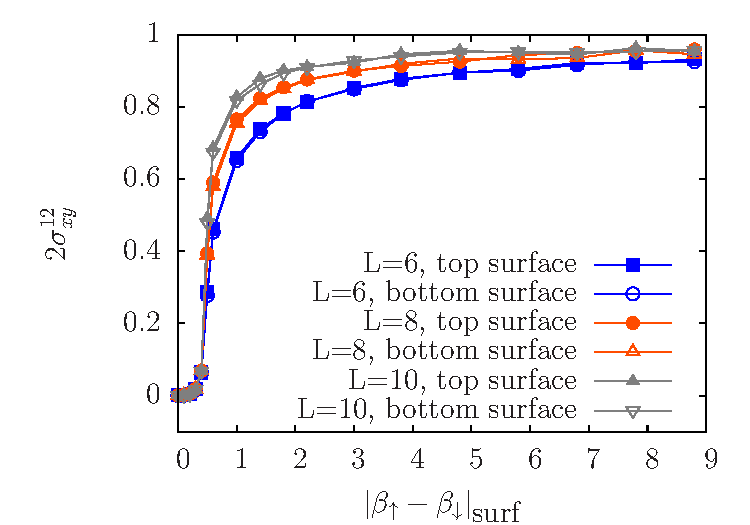
\includegraphics[width=0.6\linewidth]{figures/cp1hall.eps}
\caption{Hall conductivity on the surface of the binding phase realized in the $CP^1$ version of the model, measured in units of $e^2/h$ (see text for details). On each surface we find that the conductivity is quantized to $1$, and this odd-integer value shows that we are on the surface of a bosonic TI. Data was taken for $K=0.4$, $\lambda=8$, $\beta_\downarrow=\beta_{\rm bulk}=0.2$. We measure the same conductivity on both the top and bottom surfaces of the topological phase.
}
\label{cp1hall}
\end{figure}


%%%%%%%%%%%%%%%%%%%%%%%%%%%%%%%%%%%%%%%%%%%%%%%%%%%
\section{Realizing symmetry-enriched topological phases by binding multiple hedgehogs to a boson}
\label{section::multiple}

In all of the above sections, we have studied a system where a single boson is bound to a single hedgehog. In this section we will describe the new physics which arises when our system contains bound states of a boson and multiple hedgehogs. We induce such a binding by making the following modification to Eq.~(\ref{action}):
\begin{equation}
S=S_{\rm spin}+\frac{\lambda}{2}\sum_{r,\mu} [ dJ_\mu(r)- Q_\mu(r)]^2.
\label{cdbind}
\end{equation}
Here $d$ is an integer, and for large $\lambda$ the action will bind a boson to $d$ hedgehogs, since the $\lambda$ term is minimized by $(Q, J) = (d, 1) \times~{\rm integer}$. 

When $d\neq1$ the change of variables in Eq.~(\ref{shift}) can no longer be applied. Therefore the phase diagram in this case will be different from the $d=1$ case. We can determine the phase diagram by performing Monte Carlo simulations. As an example, the phase diagram for $d=3$ is shown in Fig.~\ref{fracphase}. Phase boundaries were determined from singularities in the specific heat. Note that in the Heisenberg model we can define a maximum of one hedgehog per lattice site, and so this model cannot easily be used to describe the binding of  multiple hedgehogs. Therefore all results for $d \neq 1$ come from the easy-plane $CP^1$ model for the spins. 

Figure~\ref{fracphase} presents the phase diagram in the variables $\lambda$ and $K$, with fixed $\beta=0.1$.
At small $\lambda$ and $K$, there is no energy cost for either hedgehogs or bosons, and they are independent. This leads to a paramagnet of spins and a superfluid of bosons. The $U(1)_{\rm spin}$ symmetry is preserved, and the $U(1)_{\rm boson}$ symmetry is broken. In contrast, at large $\lambda$ and $K$ both hedgehog and boson currents are forbidden, leading to a Coulomb phase of spins and an insulator of bosons. Here both the $U(1)_{\rm spin}$ and $U(1)_{\rm boson}$ symmetries are preserved, but the spin system has intrinsic topological order. 
At large $K$ but small $\lambda$, the Coulomb phase of the spin system survives and the hedghogs are gapped, but the bosons are condensed breaking the $U(1)_{\rm boson}$ symmetry.
On the other hand, at very small $K$ and large $\lambda$ the hedgehogs are proliferated and bosons are bound to them, and we are in the binding phase; here, neither symmetry is broken, and we will argue shortly that this is a Symmetry Enriched Topological (SET) phase. 

\begin{figure}
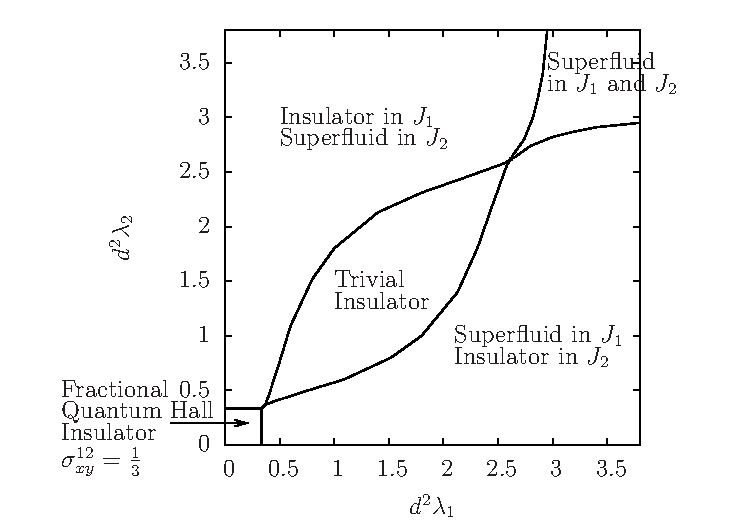
\includegraphics[angle=-90,width=0.9\linewidth]{figures/fracphase.eps}
\caption{Bulk phase diagram for the model described in Eqs.~(\ref{sspin}) and (\ref{cdbind}), with $d=3$ and small $\beta=0.1$. We can compare this to the case of $d=1$, where the middle phase is absent and the phase boundaries are straight vertical and horizontal lines; and to $d=2$, where the middle phase is absent and there is a line of phase transitions between the paramagnet/superfluid phase in the lower left corner and the Coulomb/insulator phase in the upper right corner.}
\label{fracphase}
\end{figure}

Note that similar phase diagram (at fixed small $\beta$) for $d=1$ contains only such four phases, where the binding phase is the SPT phase discussed in the previous sections. For $d=1$ these are the only phases, and due to the change of variables in Eq.~(\ref{shift}), the phase boundaries are all straight lines.
With $d\neq 1$, we have a new phase in the middle of the diagram, and no direct transition from the phase in the lower right to the binding phase. The middle phase can be understood as one in which hedgehog currents are proliferated, but their interactions are still too costly for objects with three hedgehogs and a boson to exist. Therefore such bound states are not proliferated, and individual bosons are also gapped.  We expect that this phase preserves the $U(1)$ symmetries from both the spins and bosons and is conventional paramagnet/insulator. The topological phase only arises when $K$ is lowered to the point that it does not penalize significantly objects with a hedgehog current of three and $\lambda$ is increased to strongly penalize any objects other than the $(Q, J) = (3, 1)$ bound states; at this point these bound states can form and proliferate, and the system enters the topological phase. For other values of $d$, the phase diagram is expected to have a similar form, with the exception of $d=2$, where in our studies of small system sizes the middle phase is not observed and there is a line of phase transitions between the lower left and upper right phases.

Let us now focus on the properties of the binding phase at large $\lambda$ and small $K$, which binds $d$ hedgehogs to a boson. This phase is distinct from the topological phase discussed earlier in this work. In particular, it has intrinsic topological order. Condensing bound states of $d$ hedgehogs causes the electric field lines in the phase to fractionalize, i.e., it is possible to have electric field lines of strength $1/d$. These fractionalized electric field lines are one of the gapped excitations of the system. The other elementary gapped excitation is a single hedgehog, which binds a boson charge of $1/d$. The hedgehog has well-defined statistics as it encircles the electric field lines, and we expect it to acquire a phase of $2\pi/d$ when this happens around the elementary fractionalized line. The matter fields $z_\uparrow$ and $z_\downarrow$ are confined, but still act as sources and sinks for the electric field lines of integer strength, therefore the line topological excitations in the system are only defined up to an integer, and we can say that the system has $\mathbb{Z}_d$ topological order.\cite{GukovKapustin,FracFaraday} 

In the Appendix we formally demonstrate the above properties by first removing the spinon matter fields and considering a CQED$\times U(1)_{\rm boson}$ system in which the monopoles of the compact electrodynamics are bound to bosons. Such CQED$\times U(1)_{\rm boson}$ models allow changes of variables similar to those possible in $U(1)\times U(1)$ models demonstrating SPT and SET phases of bosons in two dimensions\cite{FQHE}, which allow their properties to be readily determined. After the change of variables has been performed, we can couple the additional spinon matter fields to the CQED sector, and this gives us precisely the $CP^1\times U(1)_{\rm boson}$ model studied in this paper.

The Witten effect and Hall effect measurements can be extended to the cases with multiple hedgehogs. For the Witten effect, the amount of bound charge will be modified, since now for each hedgehog there is a boson charge of $1/d$. Therefore the screening cloud will have a charge of $1/(2d)$. We have studied the cases of $d=2, 3$ in Monte Carlo and our results, shown in Fig.~\ref{wittend}, confirm this expectation. Recall that when measuring the Witten effect we used a ``biasing'' term to break degeneracy between positive and negative internal monopoles. This biasing term may also introduces some excess internal monopole or boson charge at the location of the external monopole. This excess is screened by the surrounding system. In the $d=1$ case, we found that for most values of $\gamma$, such as those shown in Fig.~\ref{diffgamma}, the screening length is quite short and so the Witten effect can still be clearly observed. In the case of $d>1$, the screening length seems to be much larger, which can lead to fluctuations of charge larger than the Witten effect we are trying to observe. We have chosen the biasing parameter in Fig.~\ref{wittend} in such a way as to minimize these fluctuations. At other values of $\gamma$ the Witten effect can still be observed but the observation is less clear due to these fluctuations.

We have also measured the surface Hall effect upon breaking the $\ztwot$ symmetry on the surface by applying the Zeeman field as in Sec.~\ref{cp1Hall}.
Our results for the Hall conductivity are shown in Fig.~\ref{halldiff}. We find that the surface Hall conductivity is given by $1/d$, which is one-half of the value found for a two-dimensional bosonic fractional quantum Hall effect.\cite{FQHE}  We can again rationalize this observation by considering a slab of the binding phase as in Fig.~\ref{monopoles} with the opposite Zeeman fields on the two surfaces, cf.\ discussion in the paragraph preceding Eq.~(\ref{Vmn}).

\begin{figure}
\includegraphics[width=0.75\linewidth,angle=-90]{figures/wittend.eps}
\caption{Witten effect measurement, similar to Fig.~(\ref{witten}), but for the case where $d$ hedgehogs are bound to each boson. The amount of bound charge is given by $1/(2d)$, as expected (indicated by dashed lines). Parameters $K$, $\beta$ and $\lambda$ were chosen to put the bulk into the binding phase, while $\gamma$ was chosen to minimize the amount of charge away from $\scripty{r}=2$, though the value at $\scripty{r}=2$ is independent of this choice.
}
\label{wittend}
\end{figure}

\begin{figure}
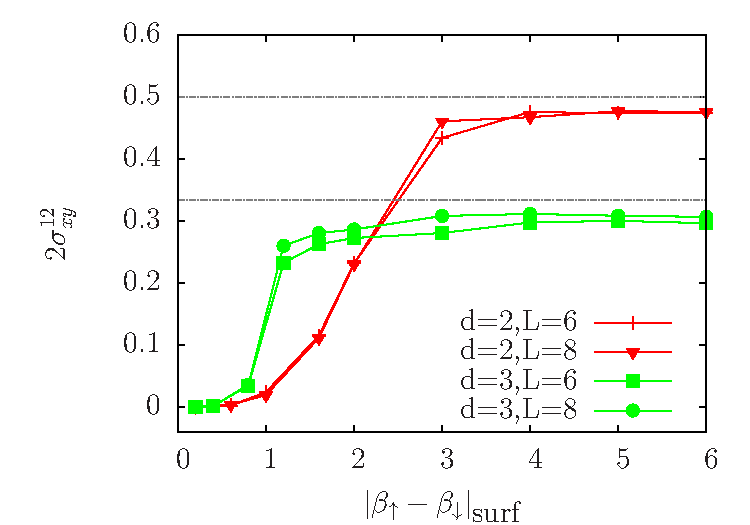
\includegraphics[width=0.6\linewidth]{figures/halldiff.eps}
\caption{Surface Hall conductivity at a boundary of an SET phase for diffent values of $d$, in units of $e^2/h$. We see that the Hall conductivity is given by $1/d$. Both surfaces have been averaged over to improve statistics. Dashed lines are drawn at $1/d$ to guide the eye. Data was taken with $K=0.2$, $\lambda=8$. Different values of $\beta_{\rm bulk}$ were used for different values of $d$, since the phase diagram changes as $d$ changes (see for example Fig.~\ref{fracphase}) and $\beta_{\rm bulk}$ needs to be chosen so that the system is in the topological phase.
}
\label{halldiff}
\end{figure}


\section{Discussion and Conclusions}
\label{sec::discussion}
In this chapter we have constructed a three-dimensional bosonic topological insulator in a lattice model which can be studied in Monte Carlo. The model works by binding bosons to point topological defects (hedgehogs). We determined the phase diagram in both the bulk and on the surface of the model. We were able to numerically extract signatures of the topological behavior: In the bulk of the model we observed a Witten effect, while on the surface with broken time-reversal symmetry we found a quantized Hall conductance with values distinct from those possible in a purely (2+1)D system. We also found other surface properties consistent with the bosonic TI, including a direct transition between surface phases with different broken symmetries, and a surface phase which breaks no symmetries and may possess topological order of a kind that would break $\ztwot$ in a purely (2+1)D system. Finally, we can also realize phases with intrinsic topological order in the bulk by binding multiple topological defects to each boson.

Our model can in principle be used to extract other properties of the bosonic topological insulator. One possible future direction is to determine the properties of the surface phase transitions, especially the transition between the two different surface superfluids. Another direction would be to find direct evidence of the exotic properties of the surface superfluids and surface topologically ordered phase. Such surface phases have generated much recent interest, as their excitations are expected to have properties not possible in a purely two-dimensional system.\cite{SenthilVishwanath,Chen2014,Cho2014} It would also be interesting to investigate the surface physics of the SET phases discussed in Sec.~\ref{section::multiple}.

In Chapter \ref{chapter::FQHE} on the two-dimensional bosonic topological phases, we were also able to reconstruct (starting from Euclidean space-time actions) explicit microscopic Hamiltonians which realized the bosonic integer and fractional quantum Hall effects. We have been unable to do the same in the present three-dimensional case, but this would be a very interesting result. More broadly, the idea of binding bosons to topological defects may continue to yield precise models of bosonic topological phases.

The model in the main text can be thought of as having either $U(1)\rtimes\ztwot$ or $U(1)\times\ztwot$ symmetry and in both cases we are realizing the same phase.
Based on the cohomology classification\cite{WenScience,WenPRB}, the symmetry $U(1)\rtimes\ztwot$ has a $\ztwo^2$ classification in three dimensions; i.e.~there are two base phases with non-trivial topology, but one of the base phases comes from $\ztwot$ only.  There is only one phase that involves $U(1)$ in a non-trivial manner, and it is this phase that we are realizing in our construction and its signature is the Witten effect, which we discuss and observe in Sec.~\ref{subsec::witten}. Our construction cannot access the phase that comes from the $\ztwot$ symmetry only because we require the $U(1)$ symmetry.
In the $U(1) \times \ztwot$ case, the cohomology classification gives $\ztwo^3$, where one of the base phases is again from the $\ztwot$ alone, while the other two base phases involve $U(1)$ in a non-trivial manner.  Of the latter two, again we are realizing the one which has the statistical Witten effect as its signature.  The other base phase does not have the Witten effect, its signature is that the monopole is the Kramers doublet under time reversal.\cite{SenthilVishwanath, BiRasmussenXu}  Our model in principle has more symmetries and could be also deformed to produce this other phase. We do not consider this here but it is a possible direction for future work.  We are also not considering beyond cohomology phases, which bring yet another phase due to $\ztwot$ only in either case.\cite{SenthilVishwanath, Kapustin2014}. 



%The Appendix contains a more abstract compact quantum electrodynamics (CQED) model where multiple hedgehogs are bound to a boson, which realizes generalizations of SPT and SET phases in more abstract settings where lattice gauge theories are included as microscopic degrees of freedom. Such generalizations have been discussed formally recently,\cite{KapustinThorngren, McGreevy, KeyserlingkBurnell2014,GukovKapustin} and similar ideas can be useful for constructing explicit models and analysing physical properties of such {phases. As a simple demonstration, in a forthcoming publication we will consider a lattice CQED model where multiple monopoles condense and lead to a novel topological phase of CQED with fractionalized Faraday lines.\cite{FracFaraday}



%%%%%%%%%%%%%%%%%%%%%%%%%%%%%%%%%%%%%%%%%%%%%%%%%%%%%%%%%%%%%%%%%%%%%%%
%\appendix
%\section{SPT- and SET-like phases in a CQED$\times$boson model in (3+1)D}
%Here we consider a model whose degrees of freedom are compact quantum electrodynamics (CQED) residing on a (3+1)-dimensional cubic space-time lattice labelled by $R$, and bosons residing on a lattice labeled by $r$.  Topological excitations in the CQED are monopoles, which are quantum particles in three spatial dimensions, and our model realizes condensation of bound states of $d$ monopoles and $c$ bosons.  We will argue that when $d=1$, these phases are analogs of Bosonic Symmetry-Protected Topological phases for such CQED$\times$boson systems and have quantized cross-transverse response given by the integer $c$.  On the other hand, when $d > 1$ these phases are analogs of Bosonic Symmetry-Enriched Topological phases and have fractional cross-transverse response given by a rational number $c/d$; these phases also feature fractionalized Faraday line excitations of the CQED and fractionalized boson particle excitations, as well as non-trivial mutual statistics between the particle and line excitations.\cite{GukovKapustin,FracFaraday}  

%While the CQED$\times$boson setting may appear artificial, this problem is relevant to the problem of SPT and SET phases of bosons in (3+1)D.  Specifically, in the main text we had a model with $U(1)\times U(1)$ symmetry, and we represented the first $U(1)$ system as an easy-plane \cp model, which has two matter fields (``spinons'') coupled to a compact gauge field.
%We then considered binding of the monopoles in the compact gauge field and physical bosons of the second $U(1)$ symmetry.  The crucial difference with the CQED$\times$boson model is the additional matter fields present in the $CP^1\times$boson model.  We will compare the systems without and with such matter fields and will argue that the matter fields destroy the distinctions of the former model, except when protected by additional discrete symmetries.

%Our CQED$\times$boson model is written in terms of compact gauge fields for the CQED part and integer-valued conserved currents for the boson part:
%\begin{widetext}
%\begin{eqnarray}
%&& Z[\hext_{\mu\nu}(R), \Aext_\rho(r)] = {\sum_{\cJ_\rho(r)}}^\prime \int_0^{2\pi} Da_\mu(R) \int_0^{2\pi} \prod_{\mu < \nu} d\gamma_{\mu\nu} \sum_{\uu_{\mu\nu}(R) = -\infty}^\infty
%e^{-S[a_\mu(R), \gamma_{\mu\nu}, \uu_{\mu\nu}(R), \cJ_\rho(r);~ \hext_{\mu\nu}(R), \Aext_\rho(r)]} ~,\label{A1}\\
%&& S \!=\! \frac{K}{2} \sum_{R, \mu < \nu} \! \left[\omega_{\mu\nu}(R) - \hext_{\mu\nu}(R) - 2\pi \uu_{\mu\nu}(R) \right]^2 
%+ \frac{\lambda}{2} \sum_{r, \rho} \left[c \cQ_\rho(r) + c \frac{\EuFrak{g}^{\rm ext}_\rho(r)}{2\pi} - d \cJ_\rho(r) \right]^2 
%\! + i \sum_{r, \rho} \cJ_\rho(r) \Aext_\rho(r) , ~~ \label{Sorig} \\
%&& \omega_{\mu\nu}(R) \equiv (\nabla_\mu a_\nu - \nabla_\nu a_\mu)(R) - \delta_{R_\mu = 0} \delta_{R_\nu = 0} \gamma_{\mu\nu} ~.
%\end{eqnarray}
%\end{widetext}
%The above action can be compared to the action of Eqs.~(\ref{sspin}) and (\ref{cdbind}) in the main text. Compared to the main text, the above action is missing the $\beta$ term which couples the gauge field to ``spinons''. We also allow the option of binding multiple bosons---here binding $c$ bosons and $d$ monopoles. The boson sector has conserved particles and is coupled to a probing field $\Aext_\rho$ in the standard way, as in the main text. Unlike the main text, the CQED sector has conserved electric field lines and is coupled to a probing rank-2 field $\hext_{\mu\nu}(R)$.  In the absence of the binding term, the coupling of the CQED sector to $\hext_{\mu\nu}$ is standard;\cite{PolyakovBook} the additional piece in the binding term, while not important for much of the discussed long-distance physics, is the correct form keeping together the ``Dirac string'' $\uu_{\mu\nu}$ and the probing field $\hext_{\mu\nu}$. Note that in the main text the additional matter fields destroy the conservation of the electric field lines, and therefore the CQED sector cannot be probed by such an external rank-2 field.
%Variables $\gamma_{\mu\nu}$ realize specific ``fluctuating boundary conditions'' in the compact gauge field variables; in a representation in terms of an integer-valued electromagnetic field tensor, this corresponds to requiring zero total field for each component.  Such details of the boundary conditions are not important for the bulk properties but are nice for a precise mathematical treatment in a system with periodic connectedness assumed here.
%From variables $B_{\mu\nu}(R)$, we define the monopole four-current $\cQ_\rho(r)$ as in Eq.~(\ref{mondef}) in the main text.
%We similarly define the four-vector $\EuFrak{g}^{\rm ext}_\rho(r)$ from $\hext_{\mu\nu}(R)$:
%\begin{equation}
%\EuFrak{g}^{\rm ext}_\rho(r) \equiv  \frac{1}{2} \epsilon_{\rho\sigma\mu\nu} \nabla_\sigma \hext_{\mu\nu} ~.
%\end{equation}
%Note that thus defined $\cQ_\rho(r)$ are conserved currents satisfying $\sum_\rho \nabla_\rho \cQ_\rho(r) = 0$, and they also satisfy the condition of zero total current in all directions: $\cQ_{{\rm tot}, \rho} \equiv \sum_r \cQ_\rho(r) = 0$.

%For the boson sector, we use a representation in terms of integer-valued conserved currents $\cJ_\rho(r)$, which satisfy $\sum_\rho \nabla_\rho \cJ_\rho(r) = 0$.  We also require that the total boson current is equal to zero for all directions, $\cJ_{{\rm tot}, \rho} = 0$.  The primed sum over $\cJ_\rho(r)$ in the partition sum signifies all such constraints.  The condition of zero total current is again convenient for precise treatment on finite systems [namely, for performing change of variables involving $\cJ$ and $\cQ$ currents, Eq.~(\ref{SL2Z}) below], while for bulk properties one can ignore these details.  The ``binding'' term parametrized by $\lambda$ is the key interaction in the action Eq.~(\ref{Sorig}) and wants to have bound states of $d$ monopoles and $c$ bosons when $\lambda$ is large [i.e., it is minimized when $(\cQ, \cJ) = (d, c) \times {\rm integer}$].  

%We first separate out the monopoles in the CQED sector as follows:
%\begin{widetext}
%\begin{eqnarray}
%\!\!\!\!\! \sum_{\uu_{\mu\nu}(R) = -\infty}^\infty \!\!\!\!\!\!\!\!\! [\dots ] \!=\!\!\!\!\!
%{\sum_{\cQ_\rho(r) = \frac{1}{2} \epsilon_{\rho\sigma\mu\nu} \nabla_\sigma \uu_{\mu\nu}^{(0)}}}^\prime \sum_{V_\mu(R) = -\infty}^\infty \sum_{\MM_{\mu\nu} = -\infty}^\infty 
%\!\!\!\!\!\![\uu_{\mu\nu}(R) = \uu_{\mu\nu}^{(0)}(R) + (\nabla_\mu V_\nu - \nabla_\nu V_\mu)(R) + \delta_{R_\mu = 0} \delta_{R_\nu = 0} \MM_{\mu\nu} ]~.
%\label{umn}
%\end{eqnarray}
%\end{widetext}
%Here $\uu_{\mu\nu}^{(0)}(R)$ is an integer-valued field whose monopolicity gives $\cQ_\rho(r)$ and is treated as a fixed function of $\cQ_\rho(r)$.  $V_\mu(R)$ and $\MM_{\mu\nu}$ are independent integer-valued fields, where the latter appear from careful treatment of the boundary conditions.  Schematically, the above arises by dividing all configurations of $\uu_{\mu\nu}(R)$ into classes defined by $\cQ_\rho(r)$ and establishing how to recover all members of a given class from one representative.  Furthermore, any $\cQ_\rho(r)$ satisfying $\sum_\rho \nabla_\rho \cQ_\rho(r) = 0$ and $\cQ_{{\rm tot}, \rho} = 0$ can be represented as above using some integer-valued $\uu_{\mu\nu}(R)$, so the primed sum over $\cQ_\rho(r)$ can be viewed as signifying these constraints.  

%A subtle point in the above is the redundancy in $V_\mu(R)$.  One way to address it precisely is as follows.  We can argue that from all links of the (3+1)D hyper-cubic lattice, we can select a subset of links such that we can take $V_\mu(R)$ as independent integer-valued variables on these links, while $V_\mu(R) = 0$ on all the other links.  We can also argue that the original CQED sector in Eq.~(\ref{A1}) can be equivalently formulated using compact gauge fields $a_\mu(R)$ that are non-zero only on exactly the same links as the independent $V_\mu(R)$.  We will assume this implicitly in all manipulations below, both for these variables and for the related variables $V_\mu^\prime(R)$, $\tilde{V}_\mu(R)$, $v_\mu(R)$, $k_{\mu}(R)$, and $\tilde{a}_\mu(R)$ that will appear below. 

%We now operate with the constrained sums over the integer-valued currents $\cQ_\rho(r)$ and $\cJ_\rho(r)$, taken to be ``outside-most'' sums in the partition sum.  We change to new independent summation variables on each link:\cite{Gen2Loops}
%\begin{equation}
%\begin{array}{c}
%\cP = a \cQ - b \cJ, \\
%\cG = c \cQ - d \cJ,
%\end{array} 
%\leftrightarrow
%\begin{array}{c}
%\cQ = d \cP - b \cG, \\
%\cJ = c \cP - a \cG ~.
%\end{array}
%\label{SL2Z}
%\end{equation}
%Here $c$ and $d$ are the same integers as in the binding term in Eq.~(\ref{Sorig}), while $a$ and $b$ are new integers such that $ad - bc = 1$, which makes the above transformation invertible in $\mathbb{Z}$.  If $c$ and $d$ are mutually prime, which we will assume throughout, we can always find such $a$ and $b$, while the arbitrariness $a \to a + kc, b \to b + kd$ does not affect any physical properties discussed below.

%The new variables $\cP_\rho(r)$ and $\cG_\rho(r)$ are also conserved integer-valued currents with zero total currents.
%For each $\cP_\rho(r)$ and $\cG_\rho(r)$, we can uniquely determine $\cQ_\rho(r)$ and hence the corresponding fixed $\uu_{\mu\nu}^{(0)}(R)$.  Let us also find for each $\cP_\rho(r)$ and $\cG_\rho(r)$ some fixed integer-valued $\uu_{P, \mu\nu}^{(0)}(R)$ and $\uu_{G, \mu\nu}^{(0)}(R)$ such that
%\begin{equation}
%\cP_\rho(r) = \frac{1}{2} \epsilon_{\rho\sigma\mu\nu} \nabla_\sigma \uu_{P, \mu\nu}^{(0)} ~, \quad 
%\cG_\rho(r) = \frac{1}{2} \epsilon_{\rho\sigma\mu\nu} \nabla_\sigma \uu_{G, \mu\nu}^{(0)} ~.
%\label{uPuG}
%\end{equation}
%We can guarantee that given the constraints satisfied by $\cP_\rho(r)$ and $\cG_\rho(r)$, such two-forms $\uu_{P, \mu\nu}^{(0)}(R)$ and $\uu_{G, \mu\nu}^{(0)}(R)$ always exist; while there are many possible choices, it does not matter which one we use as long as it stays fixed. 
%We then have
%\begin{equation}
%\epsilon_{\rho\sigma\mu\nu} \nabla_\sigma \left[\uu_{\mu\nu}^{(0)} - d \uu_{P, \mu\nu}^{(0)} + b \uu_{G, \mu\nu}^{(0)} \right] = 0 ~,
%\end{equation}
%which implies that there exist integer-valued $V^\prime_\mu(R)$, $\MM^\prime_{\mu\nu}$ such that
%\begin{eqnarray}
%\uu_{\mu\nu}^{(0)}(R) &=& d \uu_{P, \mu\nu}^{(0)}(R) - b \uu_{G, \mu\nu}^{(0)}(R) \\
%&+& (\nabla_\mu V^\prime_\nu - \nabla_\nu V^\prime_\mu)(R) + \delta_{R_\mu = 0} \delta_{R_\nu = 0} \MM^\prime_{\mu\nu} ~.\nonumber
%\end{eqnarray}
%We can again take $V^\prime_\mu(R)$, $\MM^\prime_{\mu\nu}$ as fixed functions of $\cP_\rho(r)$ and $\cG_\rho(r)$.  Now we can express $\uu_{\mu\nu}(R)$ in Eq.~(\ref{umn}) as
%\begin{eqnarray}
%\uu_{\mu\nu}(R) &=&  d \uu_{P, \mu\nu}^{(0)}(R) - b \uu_{G, \mu\nu}^{(0)}(R) \\
%&+& (\nabla_\mu \tilde{V}_\nu - \nabla_\nu \tilde{V}_\mu)(R) + \delta_{R_\mu = 0} \delta_{R_\nu = 0} \tilde{\MM}_{\mu\nu} ~,\nonumber
%\end{eqnarray}
%where we have changed the summation variables from $V_\mu(R)$, $\MM_{\mu\nu}$ to $\tilde{V}_\mu(R) = V_\mu(R) + V^\prime_\mu(R)$, $\tilde{\MM}_{\mu\nu} = \MM_{\mu\nu} + \MM^\prime_{\mu\nu}$.

%Let us write
%\begin{eqnarray}
%\tilde{V}_\mu(R) = d v_\mu(R) + k_\mu(R) ,~~
%\tilde{\MM}_{\mu\nu} = d \mm_{\mu\nu} + \ell_{\mu\nu} ,
%\end{eqnarray}
%where $v_\mu(R)$ and $\mm_{\mu\nu}$ are arbitrary integers, while $k_\mu(R)$ and $\ell_{\mu\nu}$ are integers $0, 1, \dots, d-1$. 
%Upon simple grouping of terms, we now have
%\begin{eqnarray}
%&& \omega_{\mu\nu}(R) - \hext_{\mu\nu}(R) - 2\pi \uu_{\mu\nu}(R) = \\
%&& d \left[\tilde{\omega}_{\mu\nu}(R) - \frac{1}{d} \hext_{\mu\nu}(R) + \frac{2\pi b}{d} \uu_{G, \mu\nu}^{(0)}(R) - 2\pi \tilde{\uu}_{\mu\nu}(R) \right] ~,~\nonumber
%\end{eqnarray}
%where we defined
%\begin{eqnarray}
%\tilde{\omega}_{\mu\nu}(R) &\equiv& (\nabla_\mu \tilde{a}_\nu - \nabla_\nu \tilde{a}_\mu)(R) - \delta_{R_\mu = 0} \delta_{R_\nu = 0} \tilde{\gamma}_{\mu\nu} ~,\nonumber \\
%\tilde{a}_\mu(R) &\equiv& \frac{a_\mu(R)}{d} - \frac{2\pi k_\mu(R)}{d} ~,\label{atilde} \\
%\tilde{\gamma}_{\mu\nu} &\equiv& \frac{\gamma_{\mu\nu}}{d} + \frac{2\pi \ell_{\mu\nu}}{d} ~,\nonumber \\
%\tilde{\uu}_{\mu\nu}(R) &\equiv& \uu_{P, \mu\nu}^{(0)}(R) + (\nabla_\mu v_\nu - \nabla_\nu v_\mu)(R) \nonumber \\
%&& + \delta_{R_\mu = 0} \delta_{R_\nu = 0} \mm_{\mu\nu} ~.\nonumber
%\end{eqnarray}
%Note that the integration over $a_\mu(R)$ from $0$ to $2\pi$ and summation over $k_\mu(R)$ from $0$ to $d-1$ effectively corresponds to integration over $\tilde{a}_{\mu}(R)$ from $0$ to $2\pi$.  The same holds for $\tilde{\gamma}_{\mu\nu}$.
%We can also express $\cP_\rho(r)$ from Eq.~(\ref{uPuG}) as $\cP_\rho(r) = \frac{1}{2} \epsilon_{\rho\sigma\mu\nu} \nabla_\sigma \tilde{\uu}_{\mu\nu}$ and see that $\uu_{P, \mu\nu}^{(0)}(R)$, $v_\mu(R)$, and $\mm_{\mu\nu}$ only appear in the above combination that gives $\tilde{\uu}_{\mu\nu}(R)$.  Furthermore, similarly to Eq.~(\ref{umn}), the summation over constrained $\cP_\rho(r)$ and unconstrained $v_\mu(R)$ and $\mm_{\mu\nu}$ is equivalent to a summation over unconstrained $\tilde{\uu}_{\mu\nu}$.  The partition sum becomes
%\begin{widetext}
%\begin{eqnarray}
%&& Z[\hext_{\mu\nu}(R), \Aext_\rho(r)] = {\sum_{\cG_\rho(r)}}^\prime \int_0^{2\pi} D\tilde{a}_\mu(R) \int_0^{2\pi} \prod_{\mu < \nu} d\tilde{\gamma}_{\mu\nu} \sum_{\tilde{\uu}_{\mu\nu}(R) = -\infty}^\infty 
%e^{-S[\tilde{a}_\mu(R), \tilde{\gamma}_{\mu\nu}, \tilde{\uu}_{\mu\nu}(R), \cG_\rho(r);~ \hext_{\mu\nu}(R), \Aext_\rho(r)]} ~,\\
%&& S = \frac{K d^2}{2} \sum_{R, \mu < \nu} \left[\tilde{\omega}_{\mu\nu}(R) - \frac{1}{d} \hext_{\mu\nu}(R) + \frac{2\pi b}{d} \uu_{G, \mu\nu}^{(0)}(R) - 2\pi \tilde{\uu}_{\mu\nu}(R) \right]^2 
%+ \frac{\lambda}{2} \sum_{r, \rho} \left[\cG_\rho(r) + c \frac{\EuFrak{g}^{\rm ext}_\rho(r)}{2\pi} \right]^2 \label{SKlambda} \\
%&& ~~~ + i \sum_{r, \rho} \left[c \left(\frac{1}{2} \epsilon_{\rho\sigma\mu\nu} \nabla_\sigma \tilde{\uu}_{\mu\nu} \right)(r) - a \cG_\rho(r) \right] \Aext_\rho(r) ~.\nonumber
%\end{eqnarray}
%\end{widetext}
%In this reformulation, we have a new CQED system represented by the compact gauge fields $\tilde{a}_\mu(R) \in [0, 2\pi)$ [and fluctuating boundary conditions realized with $\tilde\gamma_{\mu\nu}\in [0,2\pi)$], and a new boson system represented by the conserved current variables $\cG_\rho(r)$.  We will now argue that these new variables give a direct representation of gapped excitations in the topological phase obtained for small $K$ and large $\lambda$.  

%For a quick illustration, let us set $\Aext_\rho(r) = 0$ everywhere.  In this case, we can perform summation over $\tilde{\uu}_{\mu\nu}(R)$ independently on each placket and obtain the Villain cosine for the combination
%\begin{eqnarray}
%\!\!\!\!
%\Theta_{\mu\nu}(R) \equiv \tilde{\omega}_{\mu\nu}(R) - \frac{1}{d} \hext_{\mu\nu}(R) + \frac{2\pi b}{d} \uu_{G, \mu\nu}^{(0)}(R) ~.
%\end{eqnarray}
%Such cosine terms represent dynamics (motions) of quantum lines whose segments are created by $e^{i \tilde{a}_\mu(R)}$.  From the coupling to $\hext_{\mu\nu}(R)$, we conclude that the new lines carry electric field strength $1/d$ of the original electric field unit.  On the other hand, from the appearance of $\uu_{G, \mu\nu}^{(0)}(R)$ in $\Theta_{\mu\nu}(R)$ we conclude that the new lines ``see'' each $\cG$ particle as if it is carrying $b/d$ of monopole charge of the new CQED system.  We can state this equivalently as follows:  When a $\cG$ particle is taken around such a new line, there is a phase of $2\pi b/d$, i.e., there is non-trivial mutual statistics between the new lines and new particles.  For sufficiently small $K$ and large $\lambda$, the quantum lines created by $e^{i \tilde{a}_\mu(R)}$ and the particles represented by $\cG_\rho(r)$ are clearly gapped and are the only excitations in this phase.

%By working a bit harder and keeping track of the $\Aext$ gauge field, we can also show that the $\cG$ particles carry charge of $1/d$ with respect to $\Aext$ (i.e., we also have boson charge fractionalization in this phase if $d > 1$), and that the system has a quantized cross-transverse response characterized by a rational number $c/d$.
%First, we note that the current which couples to $\Aext_\rho(r)$ can be written as
%\begin{eqnarray*}
%c \cP_\rho(r) - a \cG_\rho(r) = c \left[\cP_\rho(r) - \frac{b}{d} \cG_\rho(r) \right] - \frac{1}{d} \cG_\rho(r) \\
%= c \left(\frac{1}{2} \epsilon_{\rho\sigma\mu\nu} \nabla_\sigma \left[\tilde{\uu}_{\mu\nu} - \frac{b}{d} \uu_{G, \mu\nu}^{(0)} \right]\right)(r) - \frac{1}{d} \cG_\rho(r) ~,
%\end{eqnarray*}
%where we used $ad - bc = 1$ and manipulated so as to separate out the same combination of $\tilde{\uu}_{\mu\nu}$ and $\uu_{G, \mu\nu}^{(0)}$ as in the $K$-term in Eq.~(\ref{SKlambda}).
%Second, on each placket $R, \mu < \nu$ we go from summation over integers $\tilde{\uu}_{\mu\nu}(R)$ to integration over real values as follows:
%\begin{equation*}
%\sum_{\tilde{\uu}_{\mu\nu}(R) = -\infty}^\infty \!\!\!\!\!\!\!\! [\dots ]
%\!=\! \int_{-\infty}^\infty \!\!\!\!\! d\tilde{\uu}_{\mu\nu}(R) \!\!\!\!\! \sum_{\tilde{F}_{\mu\nu}(R) = -\infty}^\infty \!\!\!\!\! e^{-i 2\pi \tilde{F}_{\mu\nu}(R) \tilde{\uu}_{\mu\nu}(R)} [\dots ],
%\end{equation*}
%which can be viewed as an intermediate step in a Poisson resummation from $\tilde{B}_{\mu\nu}(R)$ to $\tilde{F}_{\mu\nu}(R)$. 
%Finally, we perform Gaussian integration over the $\tilde{\uu}_{\mu\nu}(R)$, which can be simplified, e.g., by changing to new integration variable $x_{\mu\nu}(R) \equiv 2\pi \tilde{\uu}_{\mu\nu}(R) - \frac{2\pi b}{d} \uu_{G, \mu\nu}^{(0)}(R) + \frac{1}{d} \hext_{\mu\nu}(R) - \tilde{\omega}_{\mu\nu}(R)$.
%The resulting action is:
%\begin{widetext}
%\begin{eqnarray}
%S &=& \frac{1}{2 K d^2} \sum_{R, \mu < \nu} \left[\tilde{F}_{\mu\nu}(R) + c \frac{(\epsilon_{\mu\nu\sigma\rho} \nabla_\sigma \Aext_\rho)(R)}{2\pi} \right]^2
%+ i \sum_{R, \mu < \nu} \tilde{F}_{\mu\nu}(R) \tilde{\omega}_{\mu\nu}(R)
%+ \frac{\lambda}{2} \sum_{r, \rho} \left[\cG_\rho(r) + c \frac{\EuFrak{g}^{\rm ext}_\rho(r)}{2\pi} \right]^2 
%\label{S_FG_wtildea} \\
%&+& i \sum_{R, \mu < \nu} \frac{2\pi b}{d} \tilde{F}_{\mu\nu}(R) \uu_{G, \mu\nu}^{(0)}(R)
%- i \sum_{R, \mu < \nu} \frac{1}{d} \tilde{F}_{\mu\nu}(R) \hext_{\mu\nu}(R)
%- i \sum_{r, \rho} \frac{1}{d} \cG_\rho(r) \Aext_\rho(r)
%- i \sum_{r, \rho} \frac{c}{2\pi d} \Aext_\rho(r) \EuFrak{g}^{\rm ext}_\rho(r) ~.\nonumber
%\end{eqnarray}
%\end{widetext}
%We see that the formally introduced $\tilde{F}_{\mu\nu}(R)$ can be interpreted as integer-valued electromagnetic field tensor variables conjugate to the compact $\tilde{a}_\mu(R)$ variables.  Integrating out $\tilde{a}_\mu(R)$ gives ``Maxwell equations in the absence of charges'', $\sum_\nu \nabla_\nu \tilde{F}_{\mu\nu}(R) = 0$, while integrating out $\tilde{\gamma}_{\mu\nu}$ gives the condition $\sum_R \delta_{R_\mu = 0} \delta_{R_\nu = 0} \tilde{F}_{\mu\nu}(R) = 0$, which is equivalent to zero total field for each component.  For small $K$, the quantum lines whose worldsheets are represented by $\tilde{F}_{\mu\nu}(R)$ are gapped, and for large $\lambda$ the quantum particles whose worldlines are represented by $\cG_\rho(r)$ are gapped, so we have managed to express the partition sum completely in terms of gapped excitations in this phase.  From the coupling of $\tilde{F}_{\mu\nu}$ to $\hext_{\mu\nu}$ we explicitly see that the new lines carry fraction $1/d$ of the unit electric field strength, while from the coupling of $\cG_\rho$ to $\Aext_\rho$ we see that the new particles carry charge $1/d$ of the original bosons.  The coupling between $\tilde{F}_{\mu\nu}$ and $\uu_{G, \mu\nu}^{(0)}$ encodes $2\pi b/d$ statistical interaction between the new elementary line and particle excitations.  Finally, the last term $i \frac{c}{4\pi d} \sum \epsilon_{\rho\sigma\mu\nu} \Aext_\rho \nabla_\sigma \hext_{\mu\nu}$ is a property of the ``vacuum'' in these variables and represents a kind of cross-transverse response in this phase, which we see is quantized to the rational number $c/d$ in appropriate units.

%When $d=1$ we have a quantized response, but the quantum numbers of the gapped excitations are not fractionalized, and therefore we have an SPT-like phase characterized by the integer $c$. When $d>1$ the quantum numbers of gapped excitations are fractionalized, and we have intrinsic topological order and an SET-like phase.

%The cross-transverse response is due to unusual surface states when the above phase borders a trivial phase ($d=1$, $c=0$). Analysis of the surface theory in Sec.~\ref{subsec::cp1surface} can be carried over to this case in the absence of the spinon matter, and we see that the surface of the SPT-like phase $(d=1,c=1)$ in the CQED$\times$boson system has an emergent non-compact electrodynamics whose flux couples to $\Aext$ as in Eq.~(\ref{surfaceCS}). This tells us that the gapless surface mode can be viewed as a (2+1)D photon. Equivalently, the surface can be viewed as a boson system without vortices, which is always in the spin-wave phase, and therefore the (2+1)D gapless mode can also be viewed as a (2+1)D phonon.

%We can now make the connection to the $CP^1\times$boson model in the main text, which we will refer to as $U(1)_{\rm spin} \times U(1)_{\rm boson}$ model.  Here we have additional ``spinon'' matter fields coupled to the compact gauge field, schematically
%\begin{eqnarray}
%\delta S &=& S_{\rm spinons}[J_\up, J_\dn] + i \sum_{R, \mu} [J_{\up, \mu}(R) + J_{\dn, \mu}(R)] a_\mu(R),\nonumber
%\end{eqnarray}
%where $J_\up$ and $J_\dn$ are integer-valued spinon currents conjugate to the $\phi_\up$ and $\phi_\dn$ variables in Eq.~(\ref{sspin}). Using Eq.~(\ref{atilde}) and dropping all contributions of the form $i 2\pi \times$integer, we can write
%\begin{eqnarray}
%\delta S &=& S_{\rm spinons}[J_\up, J_\dn] + i d \sum_{R, \mu} [J_{\up, \mu}(R) + J_{\dn, \mu}(R)] \tilde{a}_\mu(R) ~.\nonumber
%\end{eqnarray}
%All manipulations leading to Eq.~(\ref{S_FG_wtildea}) do not touch the gauge field $\tilde{a}_\mu(R)$ and remain valid also in the presence of the spinon matter.  Now, since the original electric field lines have sources and sinks, the probing field $\hext_{\mu\nu}$ ceases to be meaningful and will be dropped; in particular, the characterization using rational $c/d$ for the cross-transverse response collapses.  On the other hand, the coupling of the new $\cG$ particles to $\Aext$ remains unaffected, and we see that they carry $1/d$ fractional charge with respect to $U(1)_{\rm boson}$.  Furthermore, upon integrating out the $\tilde{a}_\mu(R)$ fields, we now have
%\begin{equation}
%\sum_\nu \nabla_\nu \tilde{F}_{\mu\nu}(R) = -d [J_{\up, \mu}(R) + J_{\dn, \mu}(R)] ~,
%\end{equation}
%i.e., the spinons act as sources and sinks of the new field lines encoded by the integer-valued $\tilde{F}_{\mu\nu}(R)$, but these sources and sinks are in multiples of $d$.  We assume that the spinons are gapped, and they will clearly be confined in the regime of small $K$; however, they destroy the structure that we had of the integer-labeled closed lines.  Nevertheless, this destruction happens only for multiples of $d$, while it is still meaningful to talk about closed line excitations of strengths modulo $d$, i.e., we have line excitations labeled by $\mathbb{Z}_d$.  The final result is that there is no fractionalization of the $U(1)_{\rm spin}$, but we still have $\mathbb{Z}_d$ quantum line excitations and fractionalized particle excitations carrying charge $1/d$ with respect to the $U(1)_{\rm boson}$, with mutual statistics between these lines and particles. 

%Note that in either the $d=1$ or $d>1$ case, when the system contains the $U(1)_{\rm spin}$ and $\ztwot$ symmetries and $c$ is odd, the resulting phase is distinct from a phase which is a direct product of a trivial spin state times a trivial (or $1/d$ fractionalized) boson state. This distinction can be observed by measuring a quantized Witten effect as discussed in the main text. To see this one also needs to carefully include the external gauge field coupled to $U(1)_{\rm spin}$ as we did in Eq.~(\ref{withA}), particularly in the presence of external monopoles, which we did not keep track of in this Appendix.





\end{document}
